%\documentclass[twocolumn,10pt,a4paper]{article}
\documentclass[9pt]{extarticle}
\usepackage[a4paper,top=0.79in,left=0.79in,bottom=0.79in,right=0.79in]{geometry} % A4 paper margins in LibreOffice
\usepackage{hyperref}
\usepackage{amsmath}
\usepackage{amsthm}
\usepackage{amsfonts}
\usepackage{mathrsfs}
\usepackage{bm}
\usepackage{bbm}
\usepackage{ulem}
\usepackage{stmaryrd}
\usepackage{algorithm}
\usepackage{algorithmic}
\usepackage[sc]{mathpazo}
\linespread{1.05}       % Palladio needs more leading (space between lines)
\usepackage[T1]{fontenc}
\usepackage{footmisc}   % \footref, refer the same footnote at different places
\usepackage{subcaption} % sub-figures
\usepackage{setspace}   % set space between lines
\usepackage[utf8]{inputenc}
\usepackage[english]{babel}
\usepackage{xcolor}
\usepackage{graphicx}
\graphicspath{{fig/}}   % Location of the graphics files

\newtheorem{theorem}{Theorem}
\newtheorem{corollary}{Corollary}
\newtheorem{lemma}{Lemma}

\DeclareMathOperator*{\argmin}{argmin}
\DeclareMathOperator*{\argmax}{argmax}
\newcommand{\eat}[1]{}
\newcommand{\given}{\mid}
\newcommand{\llb}{\llbracket}
\newcommand{\rrb}{\rrbracket}
\newcommand{\bu}{\mathbf{u}}
\newcommand{\bv}{\mathbf{v}}
\newcommand{\x}{\mathbf{x}}
\newcommand{\y}{\mathbf{y}}
\newcommand{\w}{\mathbf{w}}
\newcommand{\p}{\mathbb{P}}
\newcommand{\q}{\mathbf{q}}
\newcommand{\alphat}{\widetilde{\alpha}}
\newcommand{\betat}{\widetilde{\beta}}
\newcommand{\gammat}{\widetilde{\gamma}}
\newcommand{\phit}{\widetilde{\phi}}

\newcommand{\eg}{e.g.\ }
\newcommand{\ie}{i.e.\ }
\newcommand{\downto}{\,\textbf{downto}\,}
\newcommand{\blue}[1]{{\color{blue}{#1}}}

\setlength{\columnsep}{1.5em} % spacing between columns

\title{The Trajectory Recommendation Problem}

\author{Dawei Chen}

\date{\today}

\begin{document}

\maketitle

\section{Problem formulation}
\label{sec:formulation}

The trajectory recommendation problem is: given a set of points-of-interest (POI) $\mathcal{P}$ and a trajectory query $\mathbf{x} = (s, K)$,
where $s \in \mathcal{P}$ is the desired start POI and $K > 1$ is the number of POIs in the desired trajectory (including the start location $s$).
We want to recommend a sequence of POIs $\mathbf{y}^*$ that maximises utility, i.e., for a suitable function $f(\cdot,\cdot)$,
\begin{equation*}
\mathbf{y}^* = \argmax_{\mathbf{y} \in \mathcal{Y}_\mathbf{x}}~f(\mathbf{x}, \mathbf{y}),
\end{equation*}
where $\mathcal{Y}_\mathbf{x}$ is the set of all possible trajectories with POIs in $\mathcal{P}$ and satisfying query $\mathbf{x}$.
$\mathbf{y} = (y_1 = s,~ y_2, \dots, y_K)$ is a trajectory with $K$ POIs, and $y_j \ne y_k$ if $j \ne k$ 
which is known as \emph{no duplicates constraint}.

Instead of the number of desired POIs, we can constrain the trajectory with a total time budget $T$.
In this case, the number of POIs $K$ can be treated as a \emph{hidden} variable, with additional constraint $\sum_{k=1}^K t_k \le T$ 
where $t_k$ is the time spent at POI $y_k$.



\subsection{A concrete example}
\label{sec:example}

Given a set of $10$ points-of-interest (POI) in Melbourne 
\begin{align*}
\mathcal{P} = \{ 
& \textit{\small Eureka Tower, Federation Square, Flinders Street Railway Station, Luna Park, Melbourne Aquarium, Melbourne Cricket Ground,} \\
& \textit{\small Melbourne Zoo, National Gallery of Victoria, Royal Exhibition Building, University of Melbourne} \}
\end{align*}
and a query $\mathbf{x} = \{\textit{\small University of Melbourne},~ 5\}$,
we would like to recommend a trajectory 
\begin{equation*}
\mathbf{y} = \{\textit{\small University of Melbourne},~ y_2, \dots, y_5\},~ y_k \in \mathcal{P},~ k=2,\dots,5.
\end{equation*}
by modelling trajectory data we have with POI and query related features as described in Section~\ref{sec:feature}.



\subsection{Related problems}
\label{sec:related}

This problem is related to automatic playlist generation, 
where we recommend a sequence of songs given a specified song (a.k.a. the seed) and the number of new songs.
Formally, given a library of songs and a query $\mathbf{x} = (s, K)$, where $s$ is the seed and $K$ is the number of songs in playlist,
we produce a list with $K$ songs (without duplication) by maximising the likelihood~\cite{chen2012playlist},
\begin{equation*}
%\max_{(y_1,\dots,y_K)} \prod_{k=2}^K \mathbb{P}(y_{k-1} \given y_k),~ y_1 = s ~\text{and}~ y_j \ne y_k,~ j \ne k.
\mathbf{y}^* = \argmax_{\mathbf{y} \in \mathcal{P}_\mathbf{x}}~ \mathbb{P}(\mathbf{y} \given \mathbf{x}),~ \mathbf{y} = (y_1=s,\dots,y_K) 
~\text{and}~ y_j \ne y_k ~\text{if}~ j \ne k.
\end{equation*}

Another similar problem is choosing a small set of photos from a large photo library and compiling them into a slideshow or movie.



\subsection{Evaluation metrics and loss functions}
\label{sec:evaluation}

To evaluate the performance of a certain recommendation algorithm,
we need to measure the similarity (or loss) given prediction $\hat{\mathbf{y}}$ and ground truth $\mathbf{y}$.
Metrics researchers have used include
\begin{itemize}
\item Hamming loss $\frac{1}{K} \sum_{j=1}^K \llb \hat{y}_j \neq y_j \rrb$, this checks if every position is the same.

\item F$_1$ score on points~\cite{ijcai15}, where we care about the set of correctly recommended POIs. 
      Let $\texttt{set}(\mathbf{y})$ denote the set of POIs in trajectory $\mathbf{y}$, F$_1$ score on points is defined as
\begin{equation*}
F_1 = \frac{2  P_{\textsc{point}}  R_{\textsc{point}}}{P_{\textsc{point}} + R_{\textsc{point}}} ~~\text{where}~
P_{\textsc{point}} = \frac{| \texttt{set}(\hat{\mathbf{y}}) \cap \texttt{set}(\mathbf{y}) |}{| \texttt{set}(\hat{\mathbf{y}}) |}~\text{and}~
R_{\textsc{point}} = \frac{| \texttt{set}(\hat{\mathbf{y}}) \cap \texttt{set}(\mathbf{y}) |}{| \texttt{set}(\mathbf{y}) |}.
\end{equation*}
If $| \hat{\mathbf{y}} | = | \mathbf{y} |$, this metric is just the unordered Hamming loss, 
i.e., Hamming loss between two binary indicator vectors of size $| \mathcal{P} |$.


\item F$_1$ score on pairs~\cite{cikm16paper}, where we care about the set of correctly predicted POI pairs,
\begin{equation*}
\text{pairs-F}_1 = \frac{2 P_{\textsc{pair}} R_{\textsc{pair}}}{P_{\textsc{pair}} + R_{\textsc{pair}}}~~\text{where}~
P_{\textsc{pair}} = \frac{N_c} {| \texttt{set}(\hat{\mathbf{y}}) | (| \texttt{set}(\hat{\mathbf{y}}) | - 1) / 2}~\text{and}~
R_{\textsc{pair}} = \frac{N_c} {| \texttt{set}(\mathbf{y}) | (| \texttt{set}(\mathbf{y}) | - 1) / 2},
\end{equation*}
and $N_c = \sum_{j=1}^{| \mathbf{y} | - 1} \sum_{k=j+1}^{| \mathbf{y} |} \llb y_j \prec_{\bar{\mathbf{y}}} y_k \rrb$,
here $y_j \prec_{\bar{\mathbf{y}}} y_k$ denotes that POI $y_j$ appears before POI $y_k$ in trajectory $\bar{\mathbf{y}}$.
We define pairs-F$_1 = 0$ when $N_c = 0$.

\end{itemize}

However, if we cast a trajectory $\mathbf{y} = (y_1,\dots,y_K)$ as a ranking of POIs in $\mathcal{P}$,
where $y_k$ has a rank $| \mathcal{P} | - k + 1$ and any other POI $p \notin \mathbf{y}$ has a rank $0$ ($0$ is an arbitrary choice).
We can make use of ranking evaluation metrics such as Kendall's $\tau$ or Spearman's $\rho$, by taking care of ties in ranks.

\eat{TODO: Write these down and contrast, esp. to pairs-F1}.



\section{Kendall's $\tau$}
\label{sec:kendalltau}

Given two ranks $X$ and $Y$, each with $n$ observations, we define
\begin{itemize}
\item Number of concordant pairs 
      \begin{equation*}
      %C = \sum_{i < j} \left( \mathbbm{1}(X_i < X_j)  \mathbbm{1}(Y_i < Y_j) + \mathbbm{1}(X_i > X_j)  \mathbbm{1}(Y_i > Y_j) \right),
      C = \frac{1}{2} \sum_{i,j} \left( \llb X_i < X_j \rrb  \llb Y_i < Y_j \rrb + \llb X_i > X_j \rrb  \llb Y_i > Y_j \rrb \right),
      \end{equation*}
      where $\llb \cdot \rrb$ is the indicator function and 
      $\sum_{i,j}$ means all unordered pairs $(i, j),~ i,j=1,\dots,n$ are counted twice.

\item Number of discordant pairs 
      \begin{equation*}
      D = \frac{1}{2} \sum_{i,j} \left( \llb X_i < X_j \rrb  \llb Y_i > Y_j \rrb + \llb X_i > X_j \rrb  \llb Y_i < Y_j \rrb \right).
      \end{equation*}

\item Number of ties in $X$
      \begin{equation*}
      T_X = \frac{1}{2} \sum_{i \ne j} \llb X_i = X_j \rrb = \sum_k \frac{t_k (t_k - 1)}{2},
      \end{equation*}
      where $t_k$ is the number of tied values in the $k$-th group of ties for $X$, for example, if
      $X = [12, 2, 1, 12, 2, 2, 1]$, there are $3$ groups of tied values, the first group is the two $12$'s, i.e., $t_1 = 2$;
      the second group is the three $2$'s, i.e., $t_2 = 3$; the third group is the two $1$'s, i.e., $t_3 = 2$. \\
      Similarly, the number of ties in $Y$ is 
      \begin{equation*}
      T_Y = \frac{1}{2} \sum_{i \ne j} \llb Y_i = Y_j \rrb = \sum_k \frac{u_k (u_k - 1)}{2},
      \end{equation*}
      where $u_k$ is the number of tied values in the $k$-th group of ties for $Y$.

\item Number of ties in both $X$ and $Y$
      \begin{equation*}
      T_{XY} = \frac{1}{2} \sum_{i \ne j} \llb X_i = X_j \rrb  \llb Y_i = Y_j \rrb.
      \end{equation*}

\item Number of ties only in $X$
      \begin{equation*}
      T = \frac{1}{2} \sum_{i \ne j} \llb X_i = X_j \rrb  \llb Y_i \ne Y_j \rrb,
      \end{equation*}
      and the number of ties only in $Y$
      \begin{equation*}
      U = \frac{1}{2} \sum_{i \ne j} \llb X_i \ne X_j \rrb  \llb Y_i = Y_j \rrb.
      \end{equation*}
\end{itemize}

Kendall's $\tau$ (version $b$) is defined as~\cite{kendall1945,agresti2010analysis} (and implemented in SciPy~\cite{scipy})
\begin{equation*}
\tau_b = \frac{C - D}{\sqrt{[n(n-1)/2 - T_X] [n(n-1)/2 - T_Y]}} = \frac{C - D}{\sqrt{(C + D + T) (C + D + U)}},
\end{equation*}
where we use equalities 
\begin{align*}
\frac{n(n-1)}{2} &= C + D + T_X + T_Y - T_{XY} \\
T &= T_X - T_{XY} \\
U &= T_Y - T_{XY}
\end{align*}



\subsection{Compare Kendall's $\tau$ with F$_1$ score on points and pairs}
\label{sec:metriccomparison}

Given a prediction $\hat{\mathbf{y}} = (\hat{y}_1, \hat{y}_2, \dots, \hat{y}_K)$ and ground truth $\mathbf{y} = (y_1, y_2, \dots, y_K)$,
for a specific ordering of POIs $(p_1, p_2, \dots, p_{|\mathcal{P}|})$,
we produce two ranks according to $\mathbf{y}$ and $\hat{\mathbf{y}}$,
\begin{align*}
r_i       &= \sum_{j=1}^K (| \mathcal{P} | - j + 1)  \llb p_i = y_j \rrb,~
i = 1, \dots, | \mathcal{P} | \\
\hat{r}_i &= \sum_{j=1}^K (| \mathcal{P} | - j + 1)  \llb p_i = \hat{y}_j \rrb,~ 
i = 1, \dots, | \mathcal{P} |
\end{align*}
where POIs not in $\mathbf{y}$ will have a rank of $0$ in $r$ and similarly in $r$.
Then we have
\begin{align*}
C &= \frac{1}{2} \sum_{i,j} \left(\llb r_i < r_j \rrb  \llb \hat{r}_i < \hat{r}_j \rrb +
     \llb r_i > r_j \rrb  \llb \hat{r}_i > \hat{r}_j \rrb \right), ~i,j = 1, \dots, | \mathcal{P} | \\
D &= \frac{1}{2} \sum_{i,j} \left(\llb r_i < r_j \rrb  \llb \hat{r}_i > \hat{r}_j \rrb +
     \llb r_i > r_j \rrb  \llb \hat{r}_i < \hat{r}_j \rrb \right), \\
T_{\mathbf{y}} &= \frac{1}{2} \sum_{i \ne j} \llb r_i = r_j \rrb 
                = \frac{1}{2} \sum_{i \ne j} \llb r_i = 0 \rrb  \llb r_j = 0 \rrb 
                = \frac{1}{2} \left( |\mathcal{P}| - K \right) \left( |\mathcal{P}| - K - 1 \right), \\ 
T_{\hat{\mathbf{y}}} &= \frac{1}{2} \sum_{i \ne j} \llb \hat{r}_i = \hat{r}_j \rrb
                      = \frac{1}{2} \sum_{i \ne j} \llb \hat{r}_i = 0 \rrb  \llb \hat{r}_j = 0 \rrb
                      = \frac{1}{2} \left( |\mathcal{P}| - K \right) \left( |\mathcal{P}| - K - 1 \right), \\ 
T_{\mathbf{y},\hat{\mathbf{y}}} &= \frac{1}{2} \sum_{i \ne j} \llb r_i = r_j \rrb  \llb \hat{r}_i = \hat{r}_j \rrb
                                 = \frac{1}{2} \sum_{i \ne j} \llb r_i = 0 \rrb  \llb r_j = 0 \rrb 
                                   \llb \hat{r}_i = 0 \rrb  \llb \hat{r}_j = 0 \rrb
                                 = \frac{1}{2} {d(d-1)},
\end{align*}
where $d = \sum_j \llb r_j = 0 \rrb  \llb \hat{r}_j = 0 \rrb$.
Kendall's $\tau$ is
\begin{equation*}
\tau_b = \frac{C - D}{\sqrt{(C + D + T) (C + D + U)}},
\end{equation*}
where $T = T_{\mathbf{y}} - T_{\mathbf{y},\hat{\mathbf{y}}}$ and $U = T_{\hat{\mathbf{y}}} - T_{\mathbf{y},\hat{\mathbf{y}}}$.
As $T_{\y} = T_{\hat\y}$, the denominator of $\tau_b$ is 
\begin{align*}
&\sqrt{(C + D + T)(C + D + U)} \\
&= \sqrt{(C + D + T_{\y} - T_{\y,\hat\y})(C + D + T_{\hat\y} - T_{\y,\hat\y})} \\
&= C + D + T_{\y} - T_{\y,\hat\y} \\
&= \frac{1}{2} \sum_{i,j} \left( \llb r_i < r_j \rrb \llb \hat{r}_i < \hat{r}_j \rrb + \llb r_i > r_j \rrb \llb \hat{r}_i > \hat{r}_j \rrb +
                                 \llb r_i < r_j \rrb \llb \hat{r}_i > \hat{r}_j \rrb + \llb r_i > r_j \rrb \llb \hat{r}_i < \hat{r}_j \rrb \right) +
   T_{\y} - T_{\y,\hat\y} \\
&= \frac{1}{2} \sum_{i,j} \left( \llb r_i < r_j \rrb + \llb r_i > r_j \rrb \right) 
                          \left( \llb \hat{r}_i < \hat{r}_j \rrb + \llb \hat{r}_i > \hat{r}_j \rrb \right) + T_{\y} - T_{\y,\hat\y} \\
&= \frac{1}{2} \sum_{i \ne j} \left( 1 - \llb r_i = r_j \rrb \right) \left( 1 - \llb \hat{r}_i = \hat{r}_j \rrb \right) + T_{\y} - T_{\y,\hat\y} \\
&= \frac{1}{2} \sum_{i \ne j} \left( 1 - \llb r_i = r_j \rrb - \llb \hat{r}_i = \hat{r}_j \rrb + 
                                         \llb r_i = r_j \rrb \llb \hat{r}_i = \hat{r}_j \rrb \right) + 
   \frac{1}{2} \sum_{i \ne j} \llb r_i = r_j \rrb - \frac{1}{2} \sum_{i \ne j} \llb r_i = r_j \rrb \llb \hat{r}_i = \hat{r}_j \rrb \\
&= \frac{1}{2} \sum_{i \ne j} 1 - \frac{1}{2} \sum_{i \ne j} \llb \hat{r}_i = \hat{r}_j \rrb \\
&= \frac{1}{2} |\mathcal{P}|(|\mathcal{P}| - 1) - \frac{1}{2} (|\mathcal{P}| - K) (|\mathcal{P}| - K - 1) \\
&= K|\mathcal{P}| - \frac{K(K + 1)}{2}
\end{align*}
So
\begin{equation*}
\tau_b = \frac{C - D}{K|\mathcal{P}| - K(K + 1)/2}
\end{equation*}

F$_1$ score on points is
\begin{equation*}
F_1 = \frac{1}{K} \sum_i \llb r_i > 0 \rrb  \llb \hat{r}_i > 0 \rrb,
\end{equation*}
and F$_1$ score on pairs is
\begin{equation*}
\text{pairs-F}_1 = \frac{\frac{1}{2} \sum_{i,j} 
                   \llb r_i < r_j \rrb  \llb r_i > 0 \rrb 
                   \llb \hat{r}_i < \hat{r}_j \rrb  \llb \hat{r}_i > 0 \rrb +
                   \frac{1}{2} \sum_{i,j} 
                   \llb r_i > r_j \rrb  \llb r_j > 0 \rrb 
                   \llb \hat{r}_i > \hat{r}_j \rrb  \llb \hat{r}_j > 0 \rrb}{K(K-1)/2}.
\end{equation*}

Define $\bar{r}_i = \llb r_i > 0 \rrb$ and $\bar{\hat{r}}_i = \llb \hat{r}_i > 0 \rrb$,
which means the values of both $\bar{r}_i$ and $\bar{\hat{r}}_i$ are binary, as a result,
the number of concordant pairs between rank $\bar{r}$ and rank $\bar{\hat{r}}$ can be written as
\begin{align*}
\bar{C} &= \frac{1}{2} \sum_{i,j} \left(
           \llb \bar{r}_i < \bar{r}_j \rrb  \llb \bar{\hat{r}}_i < \bar{\hat{r}}_j \rrb +
           \llb \bar{r}_i > \bar{r}_j \rrb  \llb \bar{\hat{r}}_i > \bar{\hat{r}}_j \rrb \right) \\
        &= \frac{1}{2} \sum_{i,j} \left(
           \llb \bar{r}_i = 0 \rrb  \llb \bar{r}_j = 1 \rrb  \llb \bar{\hat{r}}_i = 0 \rrb  \llb \bar{\hat{r}}_j = 1 \rrb +
           \llb \bar{r}_i = 1 \rrb  \llb \bar{r}_j = 0 \rrb  \llb \bar{\hat{r}}_i = 1 \rrb  \llb \bar{\hat{r}}_j = 0 \rrb \right) \\
        &= \frac{1}{2} \sum_{i,j} \left(
           \llb r_i = 0 \rrb  \llb r_j > 0 \rrb  \llb \hat{r}_i = 0 \rrb  \llb \hat{r}_j > 0 \rrb +
           \llb r_i > 0 \rrb  \llb r_j = 0 \rrb  \llb \hat{r}_i > 0 \rrb  \llb \hat{r}_j = 0 \rrb \right) \\
        &= \frac{1}{2} \sum_{i,j} \left(
           \llb r_i < r_j \rrb  \llb r_i = 0 \rrb  \llb \hat{r}_i < \hat{r}_j \rrb  \llb \hat{r}_i = 0 \rrb +
           \llb r_i > r_j \rrb  \llb r_j = 0 \rrb  \llb \hat{r}_i > \hat{r}_j \rrb  \llb \hat{r}_j = 0 \rrb \right) \\
        &= \frac{1}{2} \sum_{i,j} \llb r_i < r_j \rrb  \llb r_i = 0 \rrb  \llb \hat{r}_i < \hat{r}_j \rrb  \llb \hat{r}_i = 0 \rrb +
           \frac{1}{2} \sum_{i,j} \llb r_i > r_j \rrb  \llb r_j = 0 \rrb  \llb \hat{r}_i > \hat{r}_j \rrb  \llb \hat{r}_j = 0 \rrb \\
        &= \frac{1}{2} \sum_{i,j} \llb r_i < r_j \rrb  \llb r_i = 0 \rrb  \llb \hat{r}_i < \hat{r}_j \rrb  \llb \hat{r}_i = 0 \rrb +
           \frac{1}{2} \sum_{i,j} \llb r_j < r_i \rrb  \llb r_j = 0 \rrb  \llb \hat{r}_j < \hat{r}_i \rrb  \llb \hat{r}_j = 0 \rrb \\
        &= \sum_{i,j} \llb r_i < r_j \rrb  \llb r_i = 0 \rrb  \llb \hat{r}_i < \hat{r}_j \rrb  \llb \hat{r}_i = 0 \rrb \\
        &= \sum_{i,j} \llb r_i > r_j \rrb  \llb r_j = 0 \rrb  \llb \hat{r}_i > \hat{r}_j \rrb  \llb \hat{r}_j = 0 \rrb.
\end{align*}

Furthermore, we can rewrite the F$_1$ score on points as 
\begin{align*}
F_1 &= \frac{1}{K} \sum_i \llb r_i > 0 \rrb  \llb \hat{r}_i > 0 \rrb \\
    &= \frac{\frac{1}{K} \sum_{i,j} \llb r_i > r_j \rrb  \llb r_j = 0 \rrb  \llb \hat{r}_i > \hat{r}_j \rrb  \hat{r}_j = 0 \rrb}
            {\sum_j \llb r_j = 0 \rrb  \llb \hat{r}_j = 0 \rrb} ~~ 
            \text{as we repeatedly count the same $i$ for all $r_j = 0$ and $\hat{r}_j = 0$}, \\
    &= \frac{\bar{C}} {dK}.
\end{align*}

We can rewrite the number of concordant pairs as
\begin{align*}
C =& \frac{1}{2} \sum_{i,j} \left(\llb r_i < r_j \rrb  \llb \hat{r}_i < \hat{r}_j \rrb +
     \llb r_i > r_j \rrb  \llb \hat{r}_i > \hat{r}_j \rrb \right), \\
  =& \frac{1}{2} \sum_{i,j} \llb r_i < r_j \rrb  
     \left( \llb r_i > 0 \rrb + \llb r_i = 0 \rrb \right)  
     \llb \hat{r}_i < \hat{r}_j \rrb 
     \left( \llb \hat{r}_i > 0 \rrb + \llb \hat{r}_i = 0 \rrb \right) + \\
   & \frac{1}{2} \sum_{i,j} \llb r_i > r_j \rrb  
     \left( \llb r_j > 0 \rrb + \llb r_j = 0 \rrb \right) 
     \llb \hat{r}_i > \hat{r}_j \rrb 
     \left( \llb \hat{r}_j > 0 \rrb + \llb \hat{r}_j = 0 \rrb \right) \\
  =& \frac{1}{2} \sum_{i,j} \left( \uwave{\llb r_i < r_j \rrb  \llb r_i > 0 \rrb} +
            \llb r_i < r_j \rrb  \llb r_i = 0 \rrb \right)  
     \left( \uwave{\llb \hat{r}_i < \hat{r}_j \rrb  \llb \hat{r}_i > 0 \rrb} + 
            \llb \hat{r}_i < \hat{r}_j \rrb  \llb \hat{r}_i = 0 \rrb \right) + \\
   & \frac{1}{2} \sum_{i,j} \left( \uwave{\llb r_i > r_j \rrb  \llb r_j > 0 \rrb} + 
            \llb r_i > r_j \rrb  \llb r_j = 0 \rrb \right) 
     \left( \uwave{\llb \hat{r}_i > \hat{r}_j \rrb  \llb \hat{r}_j > 0 \rrb} + 
            \llb \hat{r}_i > \hat{r}_j \rrb  \llb \hat{r}_j = 0 \rrb \right) \\
  =& \frac{1}{2} \sum_{i,j} \uwave{\llb r_i < r_j \rrb  \llb r_i > 0 \rrb 
                         \llb \hat{r}_i < \hat{r}_j \rrb  \llb \hat{r}_i > 0 \rrb} +
     \frac{1}{2} \sum_{i,j} \uwave{\llb r_i > r_j \rrb  \llb r_j > 0 \rrb 
                         \llb \hat{r}_i > \hat{r}_j \rrb  \llb \hat{r}_j > 0 \rrb} + \\
   & \frac{1}{2} \sum_{i,j} \left( \uwave{\llb r_i < r_j \rrb  \llb r_i > 0 \rrb} 
                         \llb \hat{r}_i < \hat{r}_j \rrb  \llb \hat{r}_i = 0 \rrb + 
                         \llb r_i < r_j \rrb  \llb r_i = 0 \rrb  
                         \llb \hat{r}_i < \hat{r}_j \rrb \right) + \\ 
   & \frac{1}{2} \sum_{i,j} \left( \uwave{\llb r_i > r_j \rrb  \llb r_j > 0 \rrb} 
                         \llb \hat{r}_i > \hat{r}_j \rrb  \llb \hat{r}_j = 0 \rrb +
                         \llb r_i > r_j \rrb  \llb r_j = 0 \rrb 
                         \llb \hat{r}_i > \hat{r}_j \rrb \right) \\
  =& ~\text{pairs-F}_1  \frac{K(K-1)}{2}~ + \\
   & \frac{1}{2} \sum_{i,j} \left( \uwave{\llb r_i < r_j \rrb  \llb r_i > 0 \rrb} 
                         \llb \hat{r}_i < \hat{r}_j \rrb  \llb \hat{r}_i = 0 \rrb + 
                         \llb r_i < r_j \rrb  \llb r_i = 0 \rrb  
                         \llb \hat{r}_i < \hat{r}_j \rrb \right) + \\ 
   & \frac{1}{2} \sum_{i,j} \left( \uwave{\llb r_i > r_j \rrb  \llb r_j > 0 \rrb} 
                         \llb \hat{r}_i > \hat{r}_j \rrb  \llb \hat{r}_j = 0 \rrb +
                         \llb r_i > r_j \rrb  \llb r_j = 0 \rrb 
                         \llb \hat{r}_i > \hat{r}_j \rrb \right).
\end{align*}
We can simplify $C-D$ and $C+D$ in a similar manner,
\begin{align*}
C-D &= \frac{1}{2} \sum_{i,j} \left( \llb r_j > 0 \rrb (1 - \llb r_i > r_j \rrb) - \llb r_i > 0 \rrb (1 - \llb r_i < r_j \rrb) \right)
       \left( \llb \hat{r}_j > 0 \rrb (1 - \llb \hat{r}_i > \hat{r}_j \rrb) - \llb \hat{r}_i > 0 \rrb (1 - \llb \hat{r}_i < \hat{r}_j \rrb) \right) \\
C+D &= \frac{1}{2} \sum_{i,j} \left( \llb r_j > 0 \rrb (1 + \llb r_i > r_j \rrb) + \llb r_i > 0 \rrb (1 + \llb r_i < r_j \rrb) \right)
       \left( \llb \hat{r}_j > 0 \rrb (1 + \llb \hat{r}_i > \hat{r}_j \rrb) + \llb \hat{r}_i > 0 \rrb (1 + \llb \hat{r}_i < \hat{r}_j \rrb) \right)
\end{align*}

\section{Evaluation metrics for sequence}

In this section, we describe metrics employed to evaluate captions of images described in~\cite{chen2015microsoft},
where the goal is to evaluate the quality of a candidate caption $c_i \in C$ for an image $I_i \in I$, 
with respect to a set of reference captions $S_i = \{s_{i1},\dots,s_{im}\} \in S$.

\subsection{BLEU}
BLEU is a metric designed to evaluate machine translation.
Given candidate captions $C$ and reference captions $S$, the BLEU score is defined as
\begin{equation*}
\text{CP}_n(C, S) =
\frac{\sum_i \sum_k \min\left( h_k(c_i),~ \max_{j \in [m]} h_k(s_{ij}) \right)}
     {\sum_i \sum_k h_k(c_i)},
\end{equation*}
where $h_k(s_{ij})$ is the number of times an $n$-gram $w_k \in \Omega$ occurs in sentence $s_{ij}$,
and $k$ indexes the set of possible $n$-grams of length $n$.

{\it 
\paragraph{Q} 
To compute $h_k(s_{ij})$, is the set of $n$-grams $\Omega$ predefined? Or it is constructed from sentence $s_{ij}$?
i.e., given a sequence of $n$ items, we can construct $n$ unigrams, $n-1$ bigrams, $n-2$ trigrams and $n-k+1$ k-grams.

\paragraph{A}
$\Omega$ is predefined, specifically, we have a $\Omega$ for each value of $n$. 
For trajectory evaluation, $n=1,2$ seems good enough, which means we have $\Omega_1$ for unigrams and $\Omega_2$ for bigrams. \\
}

\noindent
It is known that CP$_n$ is a \emph{precision} score and it favors short sentences.
So a brevity penalty is used:
\begin{equation*}
b(C, S) = \begin{cases}
1 & \text{if}~ l_C > l_S \\
\exp(1-l_S/l_C) & \text{if}~ l_C \le l_S
\end{cases},
\end{equation*}
where $l_C$ is the total length of candidate sentences $c_i$'s and $l_S$ is the length of the corpus-level effective reference length.
When there are multiple references for a candidate sentence, we choose to use the \textit{closest} reference length for the brevity penalty.

{\it
\paragraph{Q}
Is $l_C = \sum_{c_i \in C} l(c_i)$?
What is the formula to compute $l_S$? 

\paragraph{A}
According to reference [39] of~\cite{chen2015microsoft}, $l_C = \sum_{i=1}^{| C |} l(c_i)$ and 
$l_S = \sum_{i=1}^{| C |} l\left( \argmin_{s \in S_i} | l(s) - l(c_i) | \right)$.
For trajectory evaluation, if the length constraint is used, we have $b(C, S) = 1$ as $l_C = l_S$. \\
}

\noindent 
The overall BLEU score is computed using a weighted geometric mean of the individual $n$-gram precision:
\begin{equation*}
\text{BLEU}_N(C, S) = b(C, S) \exp\left( \sum_{n=1}^N w_n \cdot \log \text{CP}_n(C, S) \right),
\end{equation*}
where $N=1,2,3,4$ and $w_n$ is typically held constant for all $n$.

{\it
\paragraph{Note}
If $w_n = 1/N$, the above weighted summation is geometric mean, otherwise it will be geometric mean to the power of $N w_n$.
}


\subsection{ROUGE}
ROUGE is a set of evaluation metrics designed to evaluate text summarisation algorithms.

\paragraph{ROUGE$_N$} a metric that computes $n$-gram \emph{recall} over all reference summaries given a candidate sentence,
\begin{equation*}
\text{ROUGE}_N (c_i, S_i) = \frac{\sum_j \sum_k \min\left( h_k(c_i),~ h_k(s_{ij}) \right)} {\sum_j \sum_k h_k(s_{ij})}
\end{equation*}

\paragraph{ROUGE$_L$} uses a measure based on the longest common subsequence (LCS).
Let $l(c_i, s_{ij})$ denote the length of the LCS between sentence $c_i$ and $s_{ij}$,
ROUGE$_L$ is a F-measure,
\begin{equation*}
\text{ROUGE}_L = \frac{(1 + \beta^2) R_l P_l} {R_l + \beta^2 P_l},
\end{equation*}
where $\beta$ is usually set to favour recall $R_l$ (e.g., $\beta=1.2$),
$R_l$ and $P_l$ are recall and precision of LCS defined as
\begin{equation*}
R_l = \max_j \frac{l(c_i, s_{ij})} {| s_{ij} |}, ~~
P_l = \max_j \frac{l(c_i, s_{ij})} {| c_i |}.
\end{equation*}
$n$-grams are implicit in this measure due to the use of LCS.

\paragraph{ROUGE$_S$} uses skip bigrams instead of LCS or $n$-grams. 
Skip bigrams are pairs of ordered words in a sentence where words may be skipped between pairs of words, which is similar to LCS.
Let $f_k(s_{ij})$ be the skip bigram count for sentence $s_{ij}$,
ROUGE$_S$ is defined as 
\begin{equation*}
\text{ROUGE}_S (c_i, S_i) = \frac{(1 + \beta^2) R_s P_s} {R_s + \beta^2 P_s} ~~\text{where}~~
R_s = \max_j \frac{\sum_k \min\left( f_k(c_i),~ f_k(s_{ij}) \right)} {\sum_k f_k(s_{ij})} ~~\text{and}~~
P_s = \max_j \frac{\sum_k \min\left( f_k(c_i),~ f_k(s_{ij}) \right)} {\sum_k f_k(c_i)}.
\end{equation*}
Skip bigrams are capable of capturing long range sentence structure.

{\it
\paragraph{Q} 
what is the difference between $f_1(s_{ij})$ and $f_2(s_{ij})$? i.e., the precise meaning of $k$ in $f_k(s_{ij})$.
From the Wikipedia page of $n$-gram:
A $k$-skip-$n$-gram is a length-$n$ subsequence where the components occur at distance at most $k$ from each other. 
Does it actually use $k$-skip-bigrams here?

\paragraph{A}
The $k$ here indexes the set of possible skip bigrams, like the $k$ in $h_k(c_i)$ for BLEU.
}


\subsection{METEOR}

METEOR is calculated by generating an alignment between words in candidate and reference sentences, 
the alignment is computed while minimising the number of chunks, $ch$, of the contiguous and identically ordered tokens in the sentence pair.
Given a set of alignments, $m$, 
the METEOR score is the harmonic mean of precision $P_m$ and recall $R_m$ between the best scoring reference and candidate,
\begin{equation*}
\text{METEOR} = (1 - \text{Pen}) F_\text{mean} ~~\text{where}~~
\text{Pen} = \gamma \left( \frac{ch} {m} \right)^\theta, ~~
F_\text{mean} = \frac{P_m R_m} {\alpha P_m + (1-\alpha) R_m} ~~\text{and}~~
P_m = \frac{| m |} {\sum_k h_k(c_i)},~~
R_m = \frac{| m |} {\sum_k h_k(s_{ij})}.
\end{equation*}
The METEOR score includes a penalty $\text{Pen}$ based on chunkiness of resolved matches and 
a harmonic mean term that gives the quality of the resolved matches.

{\it
\paragraph{Q}
Can we say that the alignment is computed by maximising (the product of) the length of each chunk?
What is the penalty of mismatch and gap penalty? (assuming the Needleman-Wunsch algorithm is used to do sequence alignment).

\paragraph{A}
According to reference [41] of~\cite{chen2015microsoft}, an alignment is generated by a heuristic which optimise $4$ criteria.
For trajectory evaluation, we can use the Needleman-Wunsch algorithm to minimise the edit distance, 
i.e., both the penalty of gap and that of mismatch are $1$.
}


\subsection{CIDEr}

CIDEr measure the consensus in sentences by performing a term frequency inverse document frequency (TF-IDF) weighting for each $n$-gram.
The TF-IDF weighting $g_k(s_{ij})$ for each $n$-gram $w_k$ is
\begin{equation*}
g_k(s_{ij}) = \frac{h_k(s_{ij})} {\sum_{w_l \in \Omega} h_l(s_{ij})} 
              \log \left( \frac{| I |} {\sum_{I_p \in I} \min\left( 1,~ \sum_q h_k(s_{pq}) \right)} \right).
\end{equation*}
The CIDEr$_n$ score for $n$-grams of length $n$ is computed using the average cosine similarity between candidate sentence and refrence sentences,
accounting for both precision and recall,
\begin{equation*}
\text{CIDEr}_n = 
\frac{1}{m} \sum_j 
\frac{\mathbf{g}^\mathbf{n}(c_i) \cdot \mathbf{g}^\mathbf{n}(s_{ij})} {\|\mathbf{g}^\mathbf{n}(c_i)\| \|\mathbf{g}^\mathbf{n}(s_{ij})\|},
\end{equation*}
where $\mathbf{g}^\mathbf{n}(c_i)$ is a vector formed by $g_k(c_i)$ corresponding to all $n$-grams of length $n$ and 
$\|\mathbf{g}^\mathbf{n}(c_i)\|$ is its magnitude. Scores from $n$-grams of varying lengths are combined to form the final CIDEr score,
\begin{equation*}
\text{CIDEr}(c_i, S_i) = \sum_{n=1}^N w_n \cdot \text{CIDEr}_n(c_i, S_i),
\end{equation*}
where uniform weights are used, i.e., $w_n = 1/N$ and $N=4$.

\paragraph{CIDEr-D} is a modification of CIDEr to make it more robust to gaming, 
where gaming refers to the phenomenon that a sentence poorly judged by humans tends to score highly with an automated metric.
To defend the CIDEr metric against gaming effects,
clipping and a length based Gaussian penalty were added,
\begin{equation}
\label{eq:cider-d}
\text{CIDEr-D}_n (c_i, S_i) = 
\frac{10}{m} \sum_j \exp\left( \frac{-\left( l(c_i) - l(s_{ij}) \right)^2} {2 \sigma^2} \right) \cdot
\frac{\min\left( \mathbf{g}^\mathbf{n}(c_i),~\mathbf{g}^\mathbf{n}(s_{ij}) \right) \cdot \mathbf{g}^\mathbf{n}(s_{ij})}
     {\|\mathbf{g}^\mathbf{n}(c_i)\| \|\mathbf{g}^\mathbf{n}(s_{ij})\|},
\end{equation}
where a factor of $10$ is used to make the CIDEr-D scores numerically similar to the other metrics. 
The CIDEr-D metric is computed in a similar manner to CIDEr,
\begin{equation*}
\text{CIDEr-D} = \sum_{n=1}^N w_n \cdot \text{CIDEr-D}_n(c_i, S_i).
\end{equation*}

{\it
\paragraph{Q} What is the minimum of two vectors in Equation~\ref{eq:cider-d}? Or How to compare two vectors?

\paragraph{A} There is no further explanation in reference [42] of~\cite{chen2015microsoft}, 
but the $\min$ operator in Equation~\ref{eq:cider-d} probably take element-wise minimum.
}


\subsection{Discussion}

We note that the skip bigrams in the definition of ROUGE$_S$ is similar to the pairs in Kendall's $\tau$. \\
In addition, if we consider only the neighbouring pairs in two ranks (i.e., a modified $\tau$), 
it is similar to the bigram counts in the definition of BLEU$_2$ and ROUGE$_2$. \\
It would be interesting to build connections among 
\begin{itemize}
\item BLEU$_2$ (a precision score), 
\item ROUGE$_2$ (a recall score), 
\item ROUGE$_S$, 
\item Kendall's $\tau$ and pairs-F$_1$.
\end{itemize}


\section{The cutting-plane methods}
\label{sec:cuttingplane}

The goal of cutting-plane methods is to find/localise a point in a convex \textit{target set} $Z \in \mathbb{R}^n$,
or determine that $Z$ is empty in some cases. 
The method does not assume any direct access to the description of $Z$,
such as the objective and constraint functions in an optimisation problem, except through a \textit{cutting-plane oracle}.
The method generates a query point $q$ and pass it to the oracle, 
the oracle either tells us that $q \in Z$ (in which case we are done), or it returns a hyperplane which separates $q$ from $Z$.
This hyperplane is called a \textit{cutting-plane}, or \textit{cut}, since it eliminates a half-space from our search.

Cutting-plane methods are also known as \textit{localisation} methods. 
A conceptual description of cutting-plane methods is shown in Algorithm~\ref{alg:cutting-plane}.


\begin{algorithm}[htbp]
\caption{Cutting-plane algorithm}
\label{alg:cutting-plane}
\begin{algorithmic}[1]
\STATE \textbf{Given}: an initial polyhedron $\mathcal{P}_0$ that contains $Z$.
\STATE $k = 0$
\REPEAT
    \STATE Generate a query point $q^{(k+1)}$ in $\mathcal{P}_k$
    \STATE Query the oracle at $q^{(k+1)}$
    \IF{~The oracle determines that $q^{(k+1)} \in Z$~}
        \RETURN $q^{(k+1)}$
    \ELSIF{~The oracle returns a cutting-plane $a_{k+1}^\top z \le b_{k+1}$~}
        \STATE Update constraints: $\mathcal{P}_{k+1} = \mathcal{P}_k \cap \{z | a_{k+1}^\top z \le b_{k+1} \}$
    \ENDIF
    \STATE $k = k + 1$
\UNTIL{Convergence or $\mathcal{P}_{k+1} = \emptyset$}
\end{algorithmic}
\end{algorithm}


\noindent
For a convex optimisation problem with $m$ constraints,

\begin{equation}
\label{eq:cvxprob}
\begin{aligned}
\min_{z} ~& f_0(z)        & \\
s.t.~~   ~& f_i(z) \le 0, & i = 1, \dots, m
\end{aligned} 
\end{equation}
where $f_0, \dots, f_m$ are convex and differentiable, the target set $Z$ is the optimal (or $\varepsilon$-suboptimal) set.

Given a query point $q$, the oracle first checks for feasibility.
If $q$ is not feasible, this means that at least one constraint in problem (\ref{eq:cvxprob}) is violated.
Suppose constraint $f_j(z) \le 0$ is violated by $q$, then we have $f_j(q) > 0$.
In addition, as $f_j(z)$ is convex and differentiable, we have the inequality
\begin{equation}
\label{eq:funprop}
f_j(z) \ge f_j(q) + \nabla f_j(q)^\top (z - q),~ j = 0, \dots, m
\end{equation}
We conclude that if $f_j(q) + \nabla f_j(q)^\top (z - q) > 0$, then $f_j(z) > 0$, 
which violated the constraint $f_j(z) \le 0$ in problem (\ref{eq:cvxprob}).
Thus, any feasible point should satisfy the inequality
\begin{equation}
\label{eq:feacut}
f_j(q) + \nabla f_j(q)^\top (z - q) \le 0.
\end{equation}
This is called a \textit{feasibility cut} for problem (\ref{eq:cvxprob}) since it cuts away the half-space 
$\{z | f_j(q) + \nabla f_j(q)^\top (z - q) > 0 \}$ with infeasible points.
If more than one constraint is violated by $q$, we can generate a \emph{feasibility cut} for each violated constraint.

On the other hand, if $q$ is feasible, and suppose $\nabla f_0(q) \ne 0$ (otherwise $q$ is optimal and we are done),
from Equation (\ref{eq:funprop}) we have
\begin{equation*}
f_0(z) > f_0(q), \text{~if~} \nabla f_0(q)^\top (z - q) > 0.
\end{equation*}
In other words, any point that satisfies inequality $\nabla f_0(q)^\top (z - q) > 0$ has an objective value larger than $f_0(q)$ 
and hence cannot be optimal.
It follows that we can form a cutting-plane
\begin{equation}
\label{eq:objcut}
\nabla f_0(q)^\top (z - q) \le 0,
\end{equation}
which is called an \textit{objective cut} for problem (\ref{eq:cvxprob}) and 
it cuts out the half-space $\{z | \nabla f_0(q)^\top (z - q) > 0 \}$ with non-optimal points.

If we keep track of the best (smallest) objective value for all feasible query points during the querying, i.e.,
$f_\text{best} = f_0(q_\text{best}) = \min\{f_0(q^{(t)}) | q^{(t)} ~\text{is feasible}\}$,
since the optimal point has an objective value at most $f_\text{best}$, 
we can cut away the half-space of points $\{z | f_0(z) > f_\text{best} \}$ with objective values greater than $f_\text{best}$, 
which means we add a constraint $f_0(z) \le f_\text{best}$, and from Equation~(\ref{eq:funprop}), 
we have a deep objective cut~\cite{boydlocalization},
\begin{equation}
\label{eq:deepobjcut}
f_0(q) + \nabla f_0(q)^\top (z - q) - f_\text{best} \le 0,
\end{equation}
where $q$ is the current query point and is feasible. If $q = q_\text{best}$, this cut reduces to the objective cut~(\ref{eq:objcut}).

%If $q$ is feasible and $\nabla f_0(q) = 0$ then $q$ is optimal.
For non-differentiable problems, the gradients $\nabla f_j(z)$ can generally be replaced by sub-gradients.


\subsection{Generate query points}
\label{sec:query}

We would like to generate a query point $q^{(k+1)}$ in the current polyhedron $\mathcal{P}_{k}$ such that 
the resulting cut reduces the size of $\mathcal{P}_{k+1}$ as much as possible.
However, when we query the oracle at point $q^{(k+1)}$, we do not know in which direction the generated cut will be excluded.
If we measure the informativeness of the $k$-th cut using the volume reduction ratio $\frac{V(\mathcal{P}_{k+1})}{V(\mathcal{P}_{k})}$,
we seek a point $q^{(k+1)}$ such that, no matter which direction to cut (returned by the oracle), we can obtain a certain guaranteed volume reduction.


\subsubsection{Method of Kelley-Cheney-Goldstein}
\label{sec:kcg}

Given query points $q^{(1)}, \dots, q^{(k)}$, one approach to generate the next query point $q^{(k+1)}$ is solving a linear programming (LP)
~\cite{wulff2013analytic},
\begin{equation}
\label{eq:kcg}
\begin{aligned}
\min_{z,\theta} ~& \theta  \\
s.t.~~   ~& \theta \ge f_0(q^{(i)}) + \nabla f_0(q^{(i)})^\top (z - q^{(i)}),~ \forall i \le k \\
          & A_k^\top z \le \mathbf{b}_k,
\end{aligned}
\end{equation}
where $A_k^\top z \le \mathbf{b}_k$ are the set of constraints that define polyhedron $\mathcal{P}_k$.

Let $t_i(z) = f_0(q^{(i)}) + \nabla f_0(q^{(i)})^\top (z - q^{(i)})$,
then $t_i(z)$ is a hyperplane tangent to $f_0(z)$ at point $q^{(i)}$.
We can rewrite LP (\ref{eq:kcg}) as
\begin{equation*}
\begin{aligned}
\min_{z,\theta} ~& \theta \\
s.t.~~ ~& \theta \ge \max_{z \in \mathcal{P}_k}~ t_i(z),~ i=1,\dots,k.
\end{aligned}
\end{equation*}

Let $z_i^* = \argmax_{z \in \mathcal{P}_k} t_i(z)$,
it follows that $z_i^*$ is either a vertex or a point lies on an edge of polyhedron $\mathcal{P}_k$
(this can be shown intuitively when $\mathcal{P}_k$ is a $2$-dimensional region),
and the optimal solution of LP (\ref{eq:kcg}) is $z^* = \argmax_{z_i} t_i(z_i^*)$,
it follows that the next query point $q^{(k+1)} = z^*$ is either a vertex or a point lies on an edge of $\mathcal{P}_k$.
In fact, if we solve LP (\ref{eq:kcg}) using the simplex algorithm, the optimal solution is guaranteed to be a vertex of $\mathcal{P}_k$.

In other words,
the method of \emph{Kelley-Cheney-Goldstein} is to greedily use the vertex of the current polyhedron $\mathcal{P}_k$ 
that maximise the convex objective $f_0(z)$ as the next query point.



\subsubsection{Chebyshev center method}
\label{sec:chebyshev}

If we rescale the gradients $\nabla f_0(q^{(i)})$ to unit length in problem (\ref{eq:kcg}), 
it results in finding the center of the largest Euclidean ball that lies inside the current polyhedron $\mathcal{P}_k$~\cite{elzinga1975central},
in other words, we find the next query point $q^{(k+1)}$ by solving
\begin{equation}
\label{eq:chebyshev}
\begin{aligned}
\min_{z} ~& \theta  \\
s.t.~~   ~& \theta \ge f_0(q^{(i)}) + \frac{\nabla f_0(q^{(i)})}{\|\nabla f_0(q^{(i)})\|} ^\top (z - q^{(i)}),~ \forall i \le k \\
          & A_k^\top z \le \mathbf{b}_k.
\end{aligned}
\end{equation}

This variant is called the \emph{Chebyshev center} method, which is shown to have significantly better convergence properties than the method of Kelley-Cheney-Goldstein~\cite{goffin2002convex}.


\subsubsection{Analytic center cutting plane method}
\label{sec:accpm}

Given a linear constraint $a_i^\top z \le b_i$, we define a slack variable $s_i \in \mathbb{R}$ as $s_i = b_i - a_i^\top z$,
that is, $s_i$ measures how far the current solution is from the constraint.
The analytic center is defined as the unique maximiser of the function~\cite{wulff2013analytic}
\begin{equation}
\label{eq:accpm}
\argmax_z \prod_i s_i = \argmax_z ~ \sum_{i=1}^k \log(b_i - a_i^\top z) + \sum_{j=1}^m \log(d_j - c_j^\top z),
\end{equation}
where we assume constraints $f_j(z) \le 0$ in problem (\ref{eq:cvxprob}) are linear and rewrite them as $c_j^\top z \le d_j$.
The unique maximiser of (\ref{eq:accpm}) can be efficiently found using Newton iterations~\cite{goffin2002convex}.

The analytic center cutting plane method (ACCPM) chooses the analytic center of polyhedron 
\begin{equation*}
\mathcal{P}_k = \{ z | c_j^\top z \le d_j, ~ j=1, \dots, m \text{~and~} a_i^\top z \le b_i, ~ i=1, \dots, k \}
\end{equation*}
to query the oracle.
ACCPM seems to give a good trade-off in terms of simplicity and practical performance~\cite{boydlocalization}.


\subsubsection{Center of gravity/Bayes point method}
\label{sec:cg}

Assume set $\mathcal{C} \subseteq \mathbb{R}^n$ is bounded and has nonempty interior. 
The center of gravity of $\mathcal{C}$ is defined as
\begin{equation}
\textbf{cg}(\mathcal{C}) = \frac{\int_\mathcal{C} z dz}{\int_\mathcal{C} dz}.
\end{equation}

The center of gravity (CG) method chooses the point $q^{(k+1)} = \textbf{cg}(\mathcal{P}_{k})$ to query the oracle~\cite{louche2015cutting}.
It turns out that this method has a very good convergence property in terms of the worst-case volume reduction factor,
in particular, we always have
\begin{equation}
\frac{V(\mathcal{P}_{k+1})}{V(\mathcal{P}_{k})} \le 1 - \frac{1}{e} \approx 0.63,
\end{equation}
in other words, the volume of the localisation polyhedron is reduced by at least $37\%$ at each iteration,
and this guarantee is completely independent of all problem parameters, including the dimension $n$.
However, it is \textit{extremely difficult} to compute the center of gravity of a polyhedron in $\mathbb{R}^n$, described by a set of linear inequalities,
which makes this method impractical.
Variants that compute an approximate center of gravity have been developed, and some of these approximations can be used to create a practical CG method~\cite{boydlocalization}.

\section{Training structured SVM using cutting-plane methods}
\label{sec:ssvm_train}

\subsection{Training the $n$-slack formulation of structured SVM}
\label{sec:nslackssvm}

Given $n$ training examples $(\mathbf{x}_1, \mathbf{y}_1), \dots, (\mathbf{x}_n, \mathbf{y}_n)$, 
the structured SVM with margin-rescaling\footnote{For brevity, structured SVM (SSVM) with slack-rescaling are not described in this document.}
can be formulated as a quadratic program (QP)
\begin{equation}
\label{eq:nslackform}
\begin{aligned}
\min_{\mathbf{w}, ~\bm{\xi} \ge 0} ~& \frac{1}{2} \mathbf{w}^\top \mathbf{w} + \frac{C}{n} \sum_{i=1}^n \xi_i \\
s.t.~~ ~& \mathbf{w}^\top \Psi(\mathbf{x}_i, \mathbf{y}_i) - \mathbf{w}^\top \Psi(\mathbf{x}_i, \bar{\mathbf{y}}) \ge 
       \Delta(\mathbf{y}_i, \bar{\mathbf{y}}) - \xi_i, ~(\forall i,~ \bar{\mathbf{y}} \neq \mathbf{y}_i)
\end{aligned}
\end{equation}
where $\mathbf{w}$ is the parameter vector, $C > 0$ is a regularisation constant,
$\Delta(\mathbf{y}, \bar{\mathbf{y}})$ is a discrepancy function that measures the loss 
for predicting $\bar{\mathbf{y}}$ given ground truth $\mathbf{y}$.
and $\xi_i$ is a slack variable that represents the \emph{hinge loss} associated with 
the prediction for the $i$-th example~\cite{tsochantaridis2005large},
\begin{equation}
\label{eq:nslackloss}
\xi_i = \max \left( 0,~ 
        \max_{\bar{\mathbf{y}} \in \mathcal{Y}} 
        \left\{ \Delta(\mathbf{y}_i, \bar{\mathbf{y}}) + \mathbf{w}^\top \Psi(\mathbf{x}_i, \bar{\mathbf{y}}) \right\} -
        \mathbf{w}^\top \Psi(\mathbf{x}_i, \mathbf{y}_i) \right).
\end{equation}
This formulation is called "$n$-slack" as we have one slack variable for each example in training set. \eat{citation}

To train the $n$-slack formulation of structured SVM, one option is simply enumerating all constraints and 
solve optimisation problem (\ref{eq:nslackform}) using a standard QP solver, 
however, this approach is impractical as there is a constraint for every incorrect label $\bar{\mathbf{y}}$.
Instead, we use a cutting-plane algorithm that repeatedly solves QP (\ref{eq:nslackform}) with respect to different set of constraints, 
and each iteration generates a new constraint that helps reduce the feasible region of the problem, 
until a specified precision $\varepsilon$ is achieved~\cite{joachims2009predicting}, as described in Algorithm~\ref{alg:nslacktrain}.

\begin{algorithm}[htbp]
\caption{Cutting-plane algorithm for training $n$-slack formulation of structured SVM (with margin-rescaling)}
\label{alg:nslacktrain}
\begin{algorithmic}[1]
\STATE \textbf{Input}: $\left( (\mathbf{x}_1, \mathbf{y}_1), \dots, (\mathbf{x}_n, \mathbf{y}_n) \right),~ C,~ \varepsilon$
\STATE $\mathcal{W} = \emptyset,~\mathcal{S}_i = \emptyset,~ k = 1,~ \mathbf{w}^{(k)} = \mathbf{0},~ \bm{\xi}^{(k)} = \mathbf{0}$
\REPEAT
    \FOR{$i = 1,\dots,n$}
        \STATE $\triangleright$ Query the oracle at point $q^{(k)} = (\mathbf{w}^{(k)}, \bm{\xi}^{(k)})$ as follows
        \STATE Do loss-augmented inference:~
               $\hat{\mathbf{y}}^{(k)} = \argmax_{\bar{\mathbf{y}} \in \mathcal{Y}} \{ \Delta(\mathbf{y}_i, \bar{\mathbf{y}}) + 
                \langle \mathbf{w}^{(k)},~ \Psi(\mathbf{x}_i, \bar{\mathbf{y}}) \rangle \}$ 
        \IF{~$q^{(k)}$ is not $\varepsilon$-feasible:~ 
             $\langle \mathbf{w}^{(k)},~ \Psi(\mathbf{x}_i, \mathbf{y}_i) - \Psi(\mathbf{x}_i, \hat{\mathbf{y}}^{(k)}) \rangle + 
             \varepsilon < \Delta(\mathbf{y}_i, \hat{\mathbf{y}}^{(k)}) - \xi_i^{(k)}$~}
            \STATE $\triangleright$ Form a \emph{feasibility cut} and update constraints
            \STATE $\mathcal{W} = \mathcal{W} \cup 
                    \left\{ \langle \mathbf{w},~ \Psi(\mathbf{x}_i, \mathbf{y}_i) - \Psi(\mathbf{x}_i, \hat{\mathbf{y}}^{(k)}) \rangle \ge 
                    \Delta(\mathbf{y}_i, \hat{\mathbf{y}}^{(k)}) - \xi_i \right\},~ \mathcal{S}_i = \mathcal{S}_i \cup \{\hat{\mathbf{y}}^{(k)} \}$ 
            \STATE Generate the next query point $q^{(k+1)} = (\mathbf{w}^{(k+1)}, \bm{\xi}^{(k+1)})$ 
                   by solving QP~(\ref{eq:nslackform}) w.r.t. all constraints in $\mathcal{W}$
            \STATE $k = k+1$
        \ENDIF
    \ENDFOR
%\UNTIL{$\mathcal{W}$ has not changed during iteration}
\UNTIL{$q^{(k)}$ is $\varepsilon$-feasible for all training examples}
\RETURN $q^{(k)}$
\end{algorithmic}
\end{algorithm}

Alternatively, the query point in Algorithm~\ref{alg:nslacktrain} will contain only $\mathbf{w}^{(k)}$
if we compute the loss $\xi_i^{(k)}$ on the fly~\cite{tsochantaridis2004support}
\begin{equation*}
\xi_i^{(k)} = \max \left( 0,~ 
              \max_{\bar{\mathbf{y}} \in \mathcal{S}_i} 
              \left\{ \Delta(\mathbf{y}_i, \bar{\mathbf{y}}) + \langle \mathbf{w}^{(k)}, \Psi(\mathbf{x}_i, \bar{\mathbf{y}}) \rangle \right\} -
              \langle \mathbf{w}^{(k)}, \Psi(\mathbf{x}_i, \mathbf{y}_i) \rangle \right).
\end{equation*}


\subsection{Training the $1$-slack formulation of structured SVM}
\label{sec:1slackssvm}

Another formulation of structured SVM which results in more efficient training is called "$1$-slack" formulation (with margin-rescaling),
it replaces the $n$ cutting-plane models of the hinge loss (one for each training example) with a single cutting-plane model for 
the sum of the hinge-losses~\cite{joachims2009cutting}, as a result, only one slack variable is needed,
\begin{equation}
\label{eq:1slackform}
\begin{aligned}
\min_{\mathbf{w}, ~\xi \ge 0} ~& \frac{1}{2} \mathbf{w}^\top \mathbf{w} + C \xi \\
s.t.~~ ~& \forall(\bar{\mathbf{y}}_1, \dots, \bar{\mathbf{y}}_n) \in \mathcal{Y}^n: 
          \frac{1}{n} \sum_{i=1}^n 
          \left( \mathbf{w}^\top \Psi(\mathbf{x}_i, \mathbf{y}_i) - \mathbf{w}^\top \Psi(\mathbf{x}_i, \bar{\mathbf{y}}_i) \right) \ge
          \frac{1}{n} \sum_{i=1}^n \Delta(\mathbf{y}_i, \bar{\mathbf{y}}_i) - \xi.
\end{aligned}
\end{equation}
Here the slack variable $\xi$ represents the \emph{sum of the hinge-losses} over all training examples,
\begin{equation}
\label{eq:1slackloss}
\xi = \max \left( 0,~ 
      \max_{(\bar{\mathbf{y}}_1, \dots, \bar{\mathbf{y}}_n) \in \mathcal{Y}^n} 
      \left\{ 
      \frac{1}{n} \sum_{i=1}^n \left( \Delta(\mathbf{y}_i, \bar{\mathbf{y}}_i) + \mathbf{w}^\top \Psi(\mathbf{x}_i, \bar{\mathbf{y}}_i) \right)
      \right\} - \frac{1}{n} \sum_{i=1}^n \mathbf{w}^\top \Psi(\mathbf{x}_i, \mathbf{y}_i)
      \right).
\end{equation}

Compared with the $n$-slack formulation described in Section~\ref{sec:nslackssvm}, 
the $1$-slack formulation of structured SVM increases the number of constraints exponentially~\cite{joachims2009cutting},
which means enumerating all constraints is also impractical.
Algorithm~\ref{alg:1slacktrain} described an approach similar to Algorithm~\ref{alg:nslacktrain} that uses a cutting-plane method to 
train the $1$-slack formulation of structured SVM.

\begin{algorithm}[htbp]
\caption{Cutting-plane algorithm for training $1$-slack formulation of structured SVM (with margin-rescaling)}
\label{alg:1slacktrain}
\begin{algorithmic}[1]
\STATE \textbf{Input}: $S = \left( (\mathbf{x}_1, \mathbf{y}_1), \dots, (\mathbf{x}_n, \mathbf{y}_n) \right),~ C,~ \varepsilon$
\STATE $\mathcal{W} = \emptyset$
%\REPEAT
\FOR{$k = 1,\dots,+\infty$}
    \STATE Generate query point $q^{(k)} = (\mathbf{w}^{(k)}, \xi^{(k)})$ by solving QP~(\ref{eq:1slackform}) w.r.t. all constraints in $\mathcal{W}$
    \STATE $\triangleright$ Query the oracle at point $q^{(k)}$ as follows
    \STATE Do loss-augmented inference:~
           $\hat{\mathbf{y}}_i^{(k)} = \argmax_{\bar{\mathbf{y}} \in \mathcal{Y}} \left\{ \Delta(\mathbf{y}_i, \bar{\mathbf{y}}) + 
            \langle \mathbf{w}^{(k)},~ \Psi(\mathbf{x}_i, \bar{\mathbf{y}}) \rangle \right\},~ \forall i$
    \IF{~$q^{(k)}$ is $\varepsilon$-feasible:~ $\frac{1}{n} \sum_{i=1}^n 
         \langle \mathbf{w}^{(k)},~ \Psi(\mathbf{x}_i, \mathbf{y}_i) - \Psi(\mathbf{x}_i, \hat{\mathbf{y}}_i^{(k)}) \rangle + \varepsilon \ge 
         \frac{1}{n} \sum_{i=1}^n \Delta(\mathbf{y}_i, \hat{\mathbf{y}}_i^{(k)}) - \xi^{(k)}$~}
        \RETURN $q^{(k)}$
    \ELSE
        \STATE Form a \emph{feasibility cut} and update constraints:~
               $\mathcal{W} = \mathcal{W} \cup \left\{ 
                \frac{1}{n} \sum_{i=1}^n \langle \mathbf{w},~ \Psi(\mathbf{x}_i, \mathbf{y}_i) - \Psi(\mathbf{x}_i, \hat{\mathbf{y}}_i^{(k)}) \rangle \ge 
                \frac{1}{n} \sum_{i=1}^n \Delta(\mathbf{y}_i, \hat{\mathbf{y}}_i^{(k)}) - \xi \right\}$
    \ENDIF
%\UNTIL{$\frac{1}{n} \sum_{i=1}^n 
%        \left( \mathbf{w}^\top \Psi(\mathbf{x}_i, \mathbf{y}_i) - \mathbf{w}^\top \Psi(\mathbf{x}_i, \hat{\mathbf{y}}_i) \right) + 
%        \varepsilon \ge \frac{1}{n} \sum_{i=1}^n \Delta(\mathbf{y}_i, \hat{\mathbf{y}}_i) - \xi$}
%\RETURN $(\mathbf{w}, \xi)$
\ENDFOR
\end{algorithmic}
\end{algorithm}


\section{Discussion}
\label{sec:ssvm_discussion}

From Algorithm~\ref{alg:nslacktrain} and Algorithm~\ref{alg:1slacktrain}, we observe that:
\begin{itemize}
\item To generate a query point $q$, it solves a QP with the same objective as the original optimisation problem and
      all constraints/cuts returned by previous queries. 
\item The Wolfe-dual programs of both QP (\ref{eq:nslackform}) and QP (\ref{eq:1slackform}) are QPs~\cite{tsochantaridis2005large,joachims2009cutting}.
\item All cutting-planes returned by the oracle are \emph{feasibility cuts}.
\item The training algorithm will \emph{stop} if the current query point $q$ is feasible, 
      in other words, it does not explicitly form an \emph{objective cut} when $q$ is feasible,
      which is reasonable as the algorithms optimise the objective when generating each query point.
\end{itemize}


\subsection{Query generation method}
\label{sec:ssvm_query}

Recall that in Section~\ref{sec:cuttingplane}, we have an objective $f_0(z)$ to minimise, in the case of $1$-slack formulation of structured SVM,
$f_0(z)$ is the quadratic objective in Equation~(\ref{eq:1slackform}), 
\begin{equation}
\label{eq:optobj}
f_0(z) = \frac{1}{2} \mathbf{w}^\top \mathbf{w} + C\xi,
\end{equation}
where $z = [\mathbf{w}, \xi]^\top$.
For the $n$-slack formulation, 
\begin{equation}
\begin{aligned}
f_0(z) = \frac{1}{2} \mathbf{w}^\top \mathbf{w} + \frac{C}{n} \sum_{i=1}^n \xi_i.
\end{aligned}
\end{equation}

The query point generation of both formulation of SSVM can be written as
\begin{equation*}
\begin{aligned}
\min_{z} ~& f_0(z) \\
s.t.~~ ~& A_k^\top z \le \mathbf{b}_k,
\end{aligned}
\end{equation*}
where $A_k^\top z \le \mathbf{b}_k$ is equivalent to the set of constraints in $\mathcal{W}$.


\subsection{Explicit objective cut generation}
\label{sec:ssvm_objcut}

Given query point $q = \left[ \mathbf{w}^{(k)}, \xi^{(k)} \right]^\top$, if $q$ is feasible, we can form an \emph{objective cut}
\begin{equation}
\label{eq:objcut_1slack}
\begin{aligned}
 & \nabla f_0(q)^\top (z - q) \\
=& \left[ \left[ \left.\frac{\partial f_0}{\partial \mathbf{w}}\right|_{\mathbf{w} = \mathbf{w}^{(k)}}, 
                 \left.\frac{\partial f_0}{\partial \xi}\right|_{\xi = \xi^{(k)}} \right]^\top \right]^\top 
   \left( \left[ \mathbf{w}, \xi \right]^\top - \left[ \mathbf{w}^{(k)}, \xi^{(k)} \right]^\top \right)  \\
=& \left[ \mathbf{w}^{(k)}, C \right] \left[ \mathbf{w} - \mathbf{w}^{(k)},~ \xi - \xi^{(k)} \right]^\top  \\
=& \langle \mathbf{w}^{(k)},~ \mathbf{w} - \mathbf{w}^{(k)} \rangle + C (\xi - \xi^{(k)}) \le 0.
\end{aligned}
\end{equation}

We have a similar \emph{objective cut} for the $n$-slack formulation of structured SVM
\begin{equation}
\label{eq:objcut_nslack}
\langle \mathbf{w}^{(k)}, \mathbf{w} - \mathbf{w}^{(k)} \rangle + \frac{C}{n} \sum_{i=1}^n (\xi_i - \xi_i^{(k)}) \le 0.
\end{equation}


\eat{
\subsubsection{Feasibility cut}
\label{sec:ssvm_feacut}

On the other hand, if $q = (\mathbf{w}^{(k)}, \xi^{(k)})$ is not feasible, the following constraint must be violated by $q$,
\begin{equation}
\label{eq:cut_1slackssvm}
\frac{1}{n} \sum_{i=1}^n \langle \mathbf{w},~ \Psi(\mathbf{x}_i, \mathbf{y}_i) - \Psi(\mathbf{x}_i, \hat{\mathbf{y}}_i^{(k)}) \rangle \ge 
\frac{1}{n} \sum_{i=1}^n \Delta(\mathbf{y}_i, \hat{\mathbf{y}}_i^{(k)}) - \xi.
\end{equation}
Let 
\begin{equation}
\label{eq:constraint_k}
f_k(z) = \frac{1}{n} \sum_{i=1}^n \Delta(\mathbf{y}_i, \hat{\mathbf{y}}_i^{(k)}) - 
         \frac{1}{n} \sum_{i=1}^n \langle \mathbf{w},~ \Psi(\mathbf{x}_i, \mathbf{y}_i) - \Psi(\mathbf{x}_i, \hat{\mathbf{y}}_i^{(k)}) \rangle - \xi,
\end{equation}
where $z = [\mathbf{w}, \xi]^\top$.
We can rewrite constraint (\ref{eq:cut_1slackssvm}) as $f_k(z) \le 0$.
Since $q$ violates this constraint, we can construct a \emph{feasibility cut}
\begin{equation}
\label{eq:feacut_1slack}
\begin{aligned}
 & f_k(q) + \nabla f_k(q)^\top (z - q) \\
=& f_k(q) + 
   \left[ \left[ \left.\frac{\partial f_k}{\partial \mathbf{w}}\right|_{\mathbf{w} = \mathbf{w}^{(k)}}, 
                 \left.\frac{\partial f_k}{\partial \xi}\right|_{\xi = \xi^{(k)}} \right]^\top \right]^\top 
   \left( \left[ \mathbf{w}, \xi \right]^\top - \left[ \mathbf{w}^{(k)}, \xi^{(k)} \right]^\top \right)  \\
=& f_k(q) + \left[ -\frac{1}{n} \sum_{i=1}^n \left( \Psi(\mathbf{x}_i, \mathbf{y}_i) - \Psi(\mathbf{x}_i, \hat{\mathbf{y}}_i^{(k)}) \right),  -1 \right] 
   \left[ \mathbf{w} - \mathbf{w}^{(k)},~ \xi - \xi^{(k)} \right]^\top  \\
=& \frac{1}{n} \sum_{i=1}^n \Delta(\mathbf{y}_i, \hat{\mathbf{y}}_i^{(k)}) - 
   \frac{1}{n} \sum_{i=1}^n \langle \mathbf{w}^{(k)},~ \Psi(\mathbf{x}_i, \mathbf{y}_i) - \Psi(\mathbf{x}_i, \hat{\mathbf{y}}_i^{(k)}) \rangle - 
   \xi^{(k)} + \langle -\frac{1}{n} \sum_{i=1}^n \left( \Psi(\mathbf{x}_i, \mathbf{y}_i) - \Psi(\mathbf{x}_i, \hat{\mathbf{y}}_i^{(k)}) \right),~
   \mathbf{w} - \mathbf{w}^{(k)} \rangle - \left( \xi - \xi^{(k)} \right)  \\
=& \frac{1}{n} \sum_{i=1}^n \Delta(\mathbf{y}_i, \hat{\mathbf{y}}_i^{(k)}) - 
   \frac{1}{n} \sum_{i=1}^n \langle \mathbf{w},~ \Psi(\mathbf{x}_i, \mathbf{y}_i) - \Psi(\mathbf{x}_i, \hat{\mathbf{y}}_i^{(k)}) \rangle - \xi \le 0.
\end{aligned}
\end{equation}

We found that inequalities (\ref{eq:cut_1slackssvm}) and (\ref{eq:feacut_1slack}) are identical.
This is \emph{not unexpected} as the hyperplane tangent to $f_k(z)$ (also a hyperplane) at point $q$ is \emph{identical} to hyperplane $f_k(z)$
(assuming the same domain for $z$). 

Similarly, for the $n$-slack formulation of structured SVM, 
suppose a constraint related to example $(\mathbf{x}_j, \mathbf{y}_j)$ is violated by query point $q$, 
as described in Algorithm~\ref{alg:nslacktrain}, the feasibility cut becomes
\begin{equation}
\label{eq:feacut_nslack}
g_k(z) = \Delta(\mathbf{y}_j, \hat{\mathbf{y}}^{(k)}) - 
\langle \mathbf{w},~ \Psi(\mathbf{x}_j, \mathbf{y}_j) - \Psi(\mathbf{x}_j, \hat{\mathbf{y}}^{(k)}) \rangle - \xi_j \le 0.
\end{equation}
}


\subsection{Generate query point using the method of Kelley-Cheney-Goldstein and the Chebyshev center method}
\label{sec:compare}

Suppose we use the method of Kelley-Cheney-Goldstein or the Chebyshev center method to generate query point 
when training the $1$-slack/$n$-slack formulation of structured SVM,
we can compare them with query point generation methods used in Algorithm~\ref{alg:nslacktrain} and Algorithm~\ref{alg:1slacktrain}.

Let 
\begin{align}
f_k(z) &= \frac{1}{n} \sum_{i=1}^n \Delta(\mathbf{y}_i, \hat{\mathbf{y}}_i^{(k)}) - 
          \frac{1}{n} \sum_{i=1}^n \langle \mathbf{w},~ \Psi(\mathbf{x}_i, \mathbf{y}_i) - \Psi(\mathbf{x}_i, \hat{\mathbf{y}}_i^{(k)}) \rangle - \xi
          \label{eq:constraint_k} \\
g_k(z) &= \Delta(\mathbf{y}_j, \hat{\mathbf{y}}^{(k)}) - 
          \langle \mathbf{w},~ \Psi(\mathbf{x}_j, \mathbf{y}_j) - \Psi(\mathbf{x}_j, \hat{\mathbf{y}}^{(k)}) \rangle - \xi_j \le 0 
          \label{eq:feacut_nslack}
\end{align}



\subsubsection{The $1$-slack formulation}
\label{sec:compare_1slack}

Given query points $q^{(1)}, \dots, q^{(k)}$ and the feasibility cuts returned by oracle (after querying these points), then
\begin{align*}
 & f_0(q^{(k)}) + \nabla f_0(q^{(k)})^\top (z - q^{(k)}) \\
=& \frac{1}{2} \langle \mathbf{w}^{(k)},~ \mathbf{w}^{(k)} \rangle + C\xi^{(k)} + 
   \left[ \mathbf{w}^{(k)}, C \right] \left[ \mathbf{w} - \mathbf{w}^{(k)},~ \xi - \xi^{(k)} \right]^\top  \\
=& \langle \mathbf{w}^{(k)}, \mathbf{w} \rangle - \frac{1}{2} \langle \mathbf{w}^{(k)}, \mathbf{w}^{(k)} \rangle + C\xi,
\end{align*}
where $q^{(k)} = (\mathbf{w}^{(k)}, \xi^{(k)})$ and $f_0(\cdot)$ is defined in Equation~(\ref{eq:optobj}).

If we use the method of \emph{Kelley-Cheney-Goldstein} (Section~\ref{sec:kcg}) to generate the next query point $q^{(k+1)}$,
we need to solve the following optimisation problem,
\begin{equation}
\label{eq:1slack_kcg}
\begin{aligned}
\min_{z} ~& \theta \\
s.t.~~ ~& \theta \ge \langle \mathbf{w}^{(k)}, \mathbf{w} \rangle - \frac{1}{2} \langle \mathbf{w}^{(k)}, \mathbf{w}^{(k)} \rangle + C\xi,~ \forall k \\
        & f_k(z) \le 0,~ \forall k \\
        & -\xi \le 0,
\end{aligned}
\end{equation}
where $z = [\mathbf{w}, \xi]^\top$ and $f_k(z)$ is defined in Equation~(\ref{eq:constraint_k}).

We need to solve a similar problem if we use the \emph{Chebyshev center} method (Section~\ref{sec:chebyshev}) to generate the next query point,
\begin{equation}
\label{eq:1slack_chebyshev}
\begin{aligned}
\min_{z} ~& \theta \\
s.t.~~ ~& \theta \ge 
          \frac{1}{D_k} \langle \mathbf{w}^{(k)}, \mathbf{w} \rangle + 
          (\frac{1}{2} - \frac{1}{D_k}) \langle \mathbf{w}^{(k)}, \mathbf{w}^{(k)} \rangle + 
          \frac{C}{D_k}\xi + C (1 - \frac{1}{D_k}) \xi^{(k)},~ \forall k \\
        & f_k(z) \le 0,~ \forall k \\
        & -\xi \le 0,
\end{aligned}
\end{equation}
where $D_k = \|\nabla f_0(q^{(k)})\| = \sqrt{\langle \mathbf{w}^{(k)}, \mathbf{w}^{(k)} \rangle + C^2}$ is a normalisation constant.

The method to generate the next query point used in Algorithm~\ref{alg:1slacktrain} can be rewritten as
\begin{equation}
\label{eq:1slack_query}
\begin{aligned}
\min_{z} ~& \frac{1}{2} \mathbf{w}^\top \mathbf{w} + C \xi \\
s.t.~~ ~& f_k(z) \le 0,~ \forall k \\
        & -\xi \le 0.
\end{aligned}
\end{equation}

Since $f_k(z)$ is a linear function, we know that both problem (\ref{eq:1slack_kcg}) and (\ref{eq:1slack_chebyshev}) are linear programs (LP),
and problem (\ref{eq:1slack_query}) is a quadratic program (QP). 
%We can see the difference clearly if we rewrite the objective of problem (\ref{eq:1slack_query}) to $\min_{z}\theta$ and add a new constraint
%$\theta \ge \frac{1}{2} \mathbf{w}^\top \mathbf{w} + C \xi$.
We can see the difference clearly from the \emph{epigraph form} of problem (\ref{eq:1slack_query}) 
\begin{align*}
\min_{z} ~& \theta \\
s.t.~~ ~& \theta \ge \frac{1}{2} \mathbf{w}^\top \mathbf{w} + C \xi \\
        & f_k(z) \le 0,~ \forall k \\
        & -\xi \le 0.
\end{align*}


\subsubsection{The $n$-slack formulation}
\label{sec:compare_nslack}

Similarly, for the $n$-slack formulation of structured SVM,
if we use the method of \emph{Kelley-Cheney-Goldstein} (Section~\ref{sec:kcg}) to generate the next query point $q^{(k+1)}$,
we need to solve an optimisation problem,
\begin{equation}
\label{eq:nslack_kcg}
\begin{aligned}
\min_{z} ~& \theta \\
s.t.~~ ~& \theta \ge \langle \mathbf{w}^{(k)}, \mathbf{w} \rangle - \frac{1}{2} \langle \mathbf{w}^{(k)}, \mathbf{w}^{(k)} \rangle + 
\frac{C}{n} \langle \mathbf{1}, \bm{\xi} \rangle,~ \forall k \\
        & g_k(z) \le 0,~ \forall k \\
        & -\xi_i \le 0,~ i = 1, \dots, n
\end{aligned}
\end{equation}
where $z = [\mathbf{w}, \bm{\xi}]^\top$, $\mathbf{1}$ is a $n$ dimensional vector of all $1$'s,
and $g_k(z)$ is defined in Equation~(\ref{eq:feacut_nslack}).


We need to solve a similar problem if we use the \emph{Chebyshev center} method (Section~\ref{sec:chebyshev}) to generate the next query point,
\begin{equation}
\label{eq:nslack_chebyshev}
\begin{aligned}
\min_{z} ~& \theta \\
s.t.~~ ~& \theta \ge 
          \frac{1}{G_k} \langle \mathbf{w}^{(k)}, \mathbf{w} \rangle + 
          (\frac{1}{2} - \frac{1}{G_k}) \langle \mathbf{w}^{(k)}, \mathbf{w}^{(k)} \rangle + 
          \frac{C}{nG_k} \langle \mathbf{1}, \bm{\xi} \rangle + 
          \frac{C}{n} (1 - \frac{1}{G_k}) \langle \mathbf{1}, \bm{\xi}^{(k)} \rangle,~ \forall k \\
        & g_k(z) \le 0,~ \forall k \\
        & -\xi_i \le 0,~ i = 1, \dots, n
\end{aligned}
\end{equation}
here 
$G_k 
= \sqrt{\langle \mathbf{w}^{(k)}, \mathbf{w}^{(k)} \rangle + \langle \frac{C}{n} \mathbf{1}, \frac{C}{n} \mathbf{1} \rangle} 
= \sqrt{\langle \mathbf{w}^{(k)}, \mathbf{w}^{(k)} \rangle + \frac{C^2}{n}}$
is a normalisation constant.

The method to generate the next query point used in Algorithm~\ref{alg:1slacktrain} can be rewritten (the epigraph form) as
\begin{equation}
\label{eq:nslack_genquery}
\begin{aligned}
\min_{z} ~& \theta \\
s.t.~~ ~& \theta \ge \frac{1}{2} \mathbf{w}^\top \mathbf{w} + \frac{C}{n} \langle \mathbf{1}, \bm{\xi} \rangle \\
        & g_k(z) \le 0,~ \forall k \\
        & -\xi_i \le 0.~ i = 1, \dots, n
\end{aligned}
\end{equation}

We observe similar differences as described in Section~\ref{sec:compare_1slack}.


\subsection{Efficient training via dualisation}
\label{sec:innerdual}

Recall that in Section~\ref{sec:nslackssvm}, 
the seperation oracle solves a loss-augmented inference problem for each query (Algorithm~\ref{alg:nslacktrain}),
which significantly reduces the scalability of the training algorithm.
Techniques have been developped to overcome this repeated inference, 
by exploring the dual problem of either the loss-augmented inference or 
the hinge-loss~\cite{taskar2004dissertation,taskar2005learning,meshi2010learning, bach2015paired},
which we review briefly in this section.

The $n$-slack formulation of structured SVM~(\ref{eq:nslackform}) described in Section~\ref{sec:nslackssvm} is equivalent to
\begin{align}
\min_{\mathbf{w}, ~\bm{\xi} \ge 0} ~& \frac{1}{2} \mathbf{w}^\top \mathbf{w} + \frac{C}{n} \sum_{i=1}^n \xi_i \\
s.t.~~ ~& \mathbf{w}^\top \Psi(\mathbf{x}_i, \mathbf{y}_i) + \xi_i \ge
          \max_{\bar{\mathbf{y}} \in \mathcal{Y}_i} 
          \left\{\mathbf{w}^\top \Psi(\mathbf{x}_i, \bar{\mathbf{y}}) + \Delta(\mathbf{y}_i, \bar{\mathbf{y}}) \right\},~\forall i. \label{eq:lossauginf}
\end{align}

If we can find a \emph{concise} formulation of the right-hand side of Equation~\ref{eq:lossauginf} (i.e., the loss-augmented inference),
in other words, the number of variables and constraints in the formulation is \emph{polynomial} in $L_i$, the number of variables in $\mathbf{y}_i$,
we can write its Lagrangian dual problem as 
\begin{align*}
\min_{\bm{\lambda}_i \ge \mathbf{0}} ~& h_i(\mathbf{w}, \bm{\lambda}_i) \\
s.t.~~ ~& g_i(\mathbf{w}, \bm{\lambda}_i) \le 0,
\end{align*}
where $h_i(\cdot)$ and $g_i(\cdot)$ are convex in both $\mathbf{w}$ and $\bm{\lambda}_i$.
Combining this minimisation over $\bm{\lambda}_i$ with the minimisation over $\mathbf{w}$ and $\bm{\xi}$,
we have a joint and compact convex minimisation problem
\begin{equation}
\label{eq:dualinf}
\begin{aligned}
\min_{\mathbf{w}, \bm{\xi}, \bm{\lambda}} ~& \frac{1}{2} \mathbf{w}^\top \mathbf{w} + \frac{C}{n} \sum_{i=1}^n \xi_i \\
s.t.~~ ~& \mathbf{w}^\top \Psi(\mathbf{x}_i, \mathbf{y}_i) + \xi_i \ge h_i(\mathbf{w}, \bm{\lambda}_i), ~\forall i \\
        & g_i(\mathbf{w}, \bm{\lambda}_i) \le 0, ~\forall i \\
        & \bm{\xi} \ge \mathbf{0}, ~\bm{\lambda}_i \ge \mathbf{0}, ~\forall i.
\end{aligned}
\end{equation}

Problem (\ref{eq:dualinf}) is a quadratic program with polynomial number of variables and constraints, 
and can be solved using existing off-the-shelf QP solvers.
Details of this approach are available in \cite{taskar2005learning}.


Given a hidden Markov model (HMM) with parameters $\lambda = (A, B, \pi)$,
$A = \{a_{ij}\}$, $B = \{b_j(v_k)\}$, $\pi = \{\pi_i\}$, 
state sequence $\q = q_{1:T} = q_1 q_2 \cdots q_T, \, q_t \in \{s_i\}_{i=1}^N$,
and observation sequence $O_{1:T} = O_1 O_2 \cdots O_T, \, O_t \in \{v_k\}_{k=1}^M$ and
\begin{equation}
\label{eq:notebasic}
\begin{aligned}
a_{ij} = a(s_i, s_j)   & \doteq \p(q_{t+1} = s_j |q_{t} = s_i), & 1 \le i,j \le N \\
b_j(v_k) = b(s_j, v_k) & \doteq \p(v_k |s_j),                   & 1 \le j \le N, \, 1 \le k \le M   \\
\pi_i = \pi(s_i)       & \doteq \p(q_1 = s_i),                  & 1 \le i \le N.
\end{aligned}
\end{equation}

% graphical model for HMM

% describe three problems: compute likelihood; identity the best sequence; training HMM using EM

\section{The forward procedure and Viterbi algorithm}
\label{sec:forward}

The likelihood of observation sequence $O_{1:T}$ is
\begin{align*}
\p(O_{1:T} ;\lambda) 
&= \sum_{i} \p(O_{1:T}, q_T = s_i ;\lambda) \\
&= \sum_{i} \left[ \sum_{j} \p(O_{1:T-1}, q_{T-1} = s_j ;\lambda) \cdot \p(q_T = s_i |q_{T-1} = s_j) \right] \p(O_T |q_T = s_i) \\
&= \sum_{i} \left[ \sum_{j} \p(O_{1:T-1}, q_{T-1} = s_j ;\lambda) \cdot a_{ji} \right] b_i(O_T)
\end{align*}
where we use the simplified notation $\p(O_{1:t}, q_t = s_i ;\lambda)$ to denote $\sum_{q_{1:t-1}} \p(O_{1:t}, q_{1:t-1}, q_t = s_i ;\lambda)$,
%\begin{equation}
%\label{eq:notesimp}
%\p(O_{1:t}, q_t = s_i ;\lambda) \doteq \sum_{q_{1:t-1}} \p(O_{1:t}, q_{1:t-1}, q_t = s_i ;\lambda).
%\end{equation}
and let
\begin{equation}
\label{eq:alpha}
\alpha_t(i) = \p(O_{1:t}, q_t = s_i ;\lambda) \doteq \sum_{q_{1:t-1}} \p(O_{1:t}, q_{1:t-1}, q_t = s_i ;\lambda),
\end{equation}
then the likelihood of $O_{1:T}$ is
\begin{alignat}{2}
\p(O_{1:T} ;\lambda) 
&= \sum_{i} \p(O_{1:T}, q_T = s_i ;\lambda) 
 = \blue{\sum_{i} \alpha_T(i)}  \label{eq:likelihood-forward} \\
&= \sum_{i} \left[ \sum_{j} \p(O_{1:T-1}, q_{T-1} = s_j ;\lambda) \right] a_{ji} \cdot b_i(O_T) 
 = \blue{\sum_{i} \left[ \sum_{j} \alpha_{T-1}(j) \cdot a_{ji} \right] b_i(O_T)}. \nonumber
\end{alignat}
We can repeat the above procedure to decompose $\alpha_{T-1}(j)$, in general, we have
\begin{equation}
\label{eq:forward-sum}
\alpha_t(i) = \begin{cases}
               \left[ \sum_{j} \alpha_{t-1}(j) \cdot a_{ji} \right] b_i(O_t), & t=2,\dots,T \\
               \pi_i \cdot b_i(O_t), & t=1.
              \end{cases}
\end{equation}

Computing the $\alpha_t(i)$ values by Eq.~(\ref{eq:forward-sum}) is known as the \emph{forward procedure}, 
and the likelihood of observation sequence $O_{1:T}$ can be computed using Eq.~(\ref{eq:likelihood-forward}).

To compute the highest probability state sequence $q_{1:T}^*$ given observations $O_{1:T}$, we have
\begin{equation*}
q_{1:T}^* = \argmax_{q_{1:T}} \p(O_{1:T}, q_{1:T} ;\lambda).
\end{equation*}
Observe that 
\begin{align*}
\max_{q_{1:T}} \p(O_{1:T}, q_{1:T} ;\lambda) 
&= \max_{i} \left\{ \max_{q_{1:T-1}} \p(O_{1:T}, q_{1:T-1}, q_T = s_i ;\lambda) \right\} \\
&= \max_{i} \left\{ \max_{j} \left\{ \max_{q_{1:T-2}} \p(O_{1:T-1}, q_{1:T-2}, q_{T-1} = s_j ;\lambda) \cdot 
   \p(q_T = s_i |q_{T-1} = s_j) \right\} \p(O_T |q_T = s_i) \right\} \\
&= \max_{i} \left\{ \max_{j} \left\{ \max_{q_{1:T-2}} \p(O_{1:T-1}, q_{1:T-2}, q_{T-1} = s_j ;\lambda) \cdot a_{ji} \right\} b_i(O_T) \right\}
\end{align*}
and let 
\begin{equation}
\label{eq:alphat}
\alphat_{t}(i) = \max_{q_{1:t-1}} \p(O_{1:t}, q_{1:t-1}, q_t = s_i ;\lambda),
\end{equation}
we have
\begin{alignat}{2}
\max_{q_{1:T}} \p(O_{1:T}, q_{1:T} ;\lambda) 
&= \max_{i} \left\{ \max_{q_{1:T-1}} \p(O_{1:T}, q_{1:T-1}, q_T = s_i ;\lambda) \right\} 
 = \blue{\max_{i} \alphat_{T}(i)} \label{eq:max-forward} \\
&= \max_{i} \left\{ \max_{j} \left\{ \max_{q_{1:T-2}} \p(O_{1:T-1}, q_{1:T-2}, q_{T-1} = s_j ;\lambda) \cdot a_{ji} \right\} b_i(O_T) \right\}
 = \blue{\max_{i} \left\{ \max_{j} \left\{ \alphat_{T-1}(j) \cdot a_{ji} \right\} b_i(O_T) \right\}}. \nonumber
\end{alignat}
We can repeat the above procedure to decompose $\alphat_{T-1}(j)$, in general, we have
\begin{equation}
\label{eq:forward-max}
\alphat_t(i) = \begin{cases}
                \left[ \max_{j} \alphat_{t-1}(j) \cdot a_{ji} \right] b_i(O_t), & t=2,\dots,T \\
                \pi_i \cdot b_i(O_t), & t=1.
               \end{cases}
\end{equation}

Compare Eq.~(\ref{eq:forward-sum}) with Eq.~(\ref{eq:forward-max}), 
the only difference is that Eq.~(\ref{eq:forward-max}) uses \emph{maximisation} instead of \emph{summation}.
Computing the $\alphat_t(i)$ values by Eq.~(\ref{eq:forward-max}) is known as the \emph{Viterbi algorithm}, 
and the/a sequence $\q^* = q_{1:T}^*$ with highest probability can be identified via back-tracking, and
\begin{equation}
\label{eq:alpha-sum}
\alpha_t(q_t^*) = \p(q_1^*) \cdot \p(O_1 |q_1^*) \left[ \prod_{t'=2}^t \p(q_{t'}^* |q_{t'-1}^*) \cdot \p(O_{t'} |q_{t'}^*) \right], \, t = 1,\dots,T
\end{equation}

We note that by adding a dummy state $q_{T+1} = s_{T+1}^*$ at the end of $\q$, with observation $O_{T+1}$, 
we can simplify Eq.~(\ref{eq:likelihood-forward}) and (\ref{eq:max-forward}) since dummy state $q_{T+1}$ is \emph{deterministic}:
\begin{align*}
\p(O_{1:T}; \lambda) 
&= \sum_{q_{1:T}} \p(O_{1:T+1}, q_{1:T}, q_{T+1} = s_{T+1}^*; \lambda)
 = \blue{\alpha_{T+1}(s_{T+1}^*)} \\
\max_{q_{1:T}} \p(O_{1:T}, q_{1:T}; \lambda) 
&= \max_{q_{1:T}} \p(O_{1:T+1}, q_{1:T}, q_{T+1} = s_{T+1}^*; \lambda)
 = \blue{\alphat_{T+1}(s_{T+1}^*)}
\end{align*}

\section{The backward procedure}
\label{sec:backward}

Similar to the forward procedure and the Viterbi algorithm, 
we can compute the likelihood of observations $O_{1:T}$ and identity the state sequence with highest probability by computing backwards.
By making use of conditional independences encoded by the HMM:
\begin{alignat}{2}
& q_t \perp q_{k \notin \{t-1,t\}} \mid q_{t-1} \text{~and~} q_t \perp O_{1:T} \mid q_{t-1}, \, \forall t=2,\dots,T  \label{eq:indep1} \\
& O_t \perp q_{k \ne t} \mid q_t \text{~and~} O_t \perp O_{k \ne t} \mid q_t, \, \forall t=1,\dots,T                \label{eq:indep2}
\end{alignat}
The likelihood of $O_{1:T}$ is 
\begin{align*}
\p(O_{1:T} ;\lambda) 
&= \sum_{q_{1:T}} \p(O_{1:T},q_{1:T} ;\lambda) \\
&= \sum_{i} \sum_{q_{2:T}} \p(q_1 = s_i, q_{2:T}, O_{1:T} ;\lambda) \\
&= \sum_{i} \left[ \sum_{q_{2:T}} \p(q_{2:T}, O_{2:T} |q_1 = s_i; \lambda) \right] \p(q_1 = s_i) \cdot \p(O_1 |q_1 = s_i) 
   ~~~ \text{(by Eq.~\ref{eq:indep1} and Eq.~\ref{eq:indep2})} \\
%&= \sum_{q_{2:T}} \sum_{i} \p(q_{2:T}, O_{2:T} |q_1 = s_i; \lambda) \cdot \pi_i \cdot b_i(O_1) \\
&= \sum_{i} \left[ \sum_{j} \sum_{q_{3:T}} \p(q_2 = s_j, q_{3:T}, O_{2:T} |q_1 = s_i; \lambda) \right] \pi_i \cdot b_i(O_1) \\
&= \sum_{i} \left[ \sum_{j} \left[ \sum_{q_{3:T}} \p(q_{3:T}, O_{3:T} |q_2 = s_j; \lambda) \right] \p(q_2 = s_j |q_1 = s_i) \cdot \p(O_2 |q_2 = s_j) 
   \right] \pi_i \cdot b_i(O_1) 
   ~~~ \text{(by Eq.~\ref{eq:indep1} and Eq.~\ref{eq:indep2})}
%&= \sum_{i} \left[ \sum_{j} \left[ \sum_{q_{3:T}} \p(q_{3:T}, O_{3:T} |q_2 = s_j; \lambda) \right] a_{ij} \cdot b_j(O_2) \right] \pi_i \cdot b_i(O_1) 
\end{align*}

%Let $\beta_t(i) = \p(O_{t+1:T} |q_t = s_i; \lambda)$ with notation simplification
%\p(O_{t+1:T} |q_t = s_i; \lambda) \doteq \sum_{q_{t+1:T}} \p(q_{t+1:T}, O_{t+1:T} |q_t = s_i; \lambda),

Let 
\begin{equation}
\label{eq:beta}
\beta_t(i) = \p(O_{t+1:T} |q_t = s_i; \lambda) \doteq \sum_{q_{t+1:T}} \p(q_{t+1:T}, O_{t+1:T} |q_t = s_i; \lambda),
\end{equation}
with notation simplification similar to Eq.~(\ref{eq:alpha}), we have
\begin{alignat}{2}
\p(O_{1:T} ;\lambda) 
&= \sum_{i} \left[ \sum_{q_{2:T}} \p(q_{2:T}, O_{2:T} |q_1 = s_i; \lambda) \right] \pi_i \cdot b_i(O_1) 
 = \blue{\sum_{i} \beta_1(i) \cdot \pi_i \cdot b_i(O_1)}  \label{eq:likelihood-backward} \\
&= \sum_{i} \left[ \sum_{j} \left[ \sum_{q_{3:T}} \p(q_{3:T}, O_{3:T} |q_2 = s_j; \lambda) \right] a_{ij} \cdot b_j(O_2) \right] \pi_i \cdot b_i(O_1) 
 = \blue{\sum_{i} \left[ \sum_{j} \beta_2(j) \cdot a_{ij} \cdot b_j(O_2) \right] \pi_i \cdot b_i(O_1)}  \nonumber
\end{alignat}
We can repeat the above procedure to decompose $\beta_2(j)$, in general, we have
\begin{equation}
\label{eq:backward-sum}
\beta_t(i) = \begin{cases}
              1, & t=T \\
              \sum_{j} \beta_{t+1}(j) \cdot a_{ij} \cdot b_j(O_{t+1}), & t=T\!-\!1 \downto 1.
             \end{cases}
\end{equation}

Computing the $\beta_t(i)$ values by Eq.~(\ref{eq:backward-sum}) is known as the \emph{backward procedure}, 
and the likelihood of observation sequence $O_{1:T}$ can be computed using Eq.~(\ref{eq:likelihood-backward}).

Similarly, to identity the highest probability state sequence $q_{1:T}^*$ given observations $O_{1:T}$, 
we observe that 
\begin{align*}
\max_{q_{1:T}} \p(O_{1:T}, q_{1:T} ;\lambda) 
&= \max_{i} \max_{q_{2:T}} \p(q_1 = s_i, q_{2:T}, O_{1:T} ;\lambda) \\
&= \max_{i} \left\{ \max_{q_{2:T}} \p(q_{2:T}, O_{2:T} |q_1 = s_i; \lambda) \right\} \p(q_1 = s_i) \cdot \p(O_1 |q_1 = s_i) 
   ~~~ \text{(by Eq.~\ref{eq:indep1} and Eq.~\ref{eq:indep2})} \\
&= \max_{i} \left\{ \max_{j} \max_{q_{3:T}} \p(q_2 = s_j, q_{3:T}, O_{2:T} |q_1 = s_i; \lambda) \right\} \pi_i \cdot b_i(O_1) \\
&= \max_{i} \left\{ \max_{j} \left\{ \max_{q_{3:T}} \p(q_{3:T}, O_{3:T} |q_2 = s_j; \lambda) \right\} \p(q_2 = s_j |q_1 = s_i) \cdot \p(O_2 |q_2 = s_j) 
   \right\} \pi_i \cdot b_i(O_1) 
   ~~~ \text{(by Eq.~\ref{eq:indep1} and Eq.~\ref{eq:indep2})}
\end{align*}
Let 
\begin{equation}
\label{eq:betat}
\betat_t(i) = \max_{q_{t+1:T}} \p(q_{t+1:T}, O_{t+1:T} |q_t = s_i; \lambda),
\end{equation}
we have
\begin{alignat}{2}
\max_{q_{1:T}} \p(O_{1:T}, q_{1:T} ;\lambda) 
&= \max_{i} \left\{ \max_{q_{2:T}} \p(q_{2:T}, O_{2:T} |q_1 = s_i; \lambda) \right\} \pi_i \cdot b_i(O_1) 
 = \blue{\max_{i} \betat_1(i) \cdot \pi_i \cdot b_i(O_1)}  \label{eq:max-backward}\\
&= \max_{i} \left\{ \max_{j} \left\{ \max_{q_{3:T}} \p(q_{3:T}, O_{3:T} |q_2 = s_j; \lambda) \right\} a_{ij} \cdot b_j(O_2) \right\} \pi_i \cdot b_i(O_1) 
 = \blue{\max_{i} \left\{ \max_{j} \betat_2(j) \cdot a_{ij} \cdot b_j(O_2) \right\} \pi_i \cdot b_i(O_1)}  \nonumber
\end{alignat}
We can repeat the above procedure to decompose $\betat_2(j)$, in general, we have
\begin{equation}
\label{eq:backward-max}
\betat_t(i) = \begin{cases}
              1, & t=T \\
              \max_{j} \betat_{t+1}(j) \cdot a_{ij} \cdot b_j(O_{t+1}), & t=T\!-\!1 \downto 1.
             \end{cases}
\end{equation}

Compare Eq.~(\ref{eq:backward-sum}) with Eq.~(\ref{eq:backward-max}), 
the only difference is that Eq.~(\ref{eq:backward-max}) uses \emph{maximisation} instead of \emph{summation} (used in Eq.~\ref{eq:backward-sum}).
It is also interesting to compare Eq.~(\ref{eq:forward-max}) with Eq.~(\ref{eq:backward-max}), 
the latter can be treated as the Viterbi algorithm works backwards, 
and the/a sequence $q_{1:T}^*$ with highest probability can be identified via \emph{forward}-tracking, and
\begin{equation}
\label{eq:beta-sum}
\betat_t(s_i) = \frac{\p(q_{t+1}^* |s_i)} {\p(q_{t+1}^* |q_t^*)} \prod_{k=t}^{T-1} \p(q_{k+1}^* |q_{k}^*) \cdot \p(O_{k+1} |q_{k+1}^*), \, t = 1,\dots,T\!-\!1
\end{equation}

We also note that by adding a dummy state $q_0 = s_0^*$ at the front of $\q$, with observation $O_0$, 
we can simplify Eq.~(\ref{eq:likelihood-backward}) and (\ref{eq:max-backward}) since dummy state $q_0$ is \emph{deterministic}:
\begin{align*}
\p(O_{1:T} ;\lambda) 
&= \sum_{q_{1:T}} \p(O_{0:T}, q_0 = s_0^*, q_{1:T}; \lambda)
 = \sum_{q_{1:T}} \p(O_{1:T}, q_{1:T} |q_0 = s_0^*; \lambda)
 = \blue{\beta_0(s_0^*)} \\
\max_{q_{1:T}} \p(O_{1:T}, q_{1:T}; \lambda) 
&= \max_{q_{1:T}} \p(O_{0:T}, q_0 = s_0^*, q_{1:T}; \lambda)
 = \max_{q_{1:T}} \p(O_{1:T}, q_{1:T} |q_0 = s_0^*; \lambda)
 = \blue{\betat_0(s_0^*)}
\end{align*}

\section{The list Viterbi algorithm}
\label{sec:lva}

Let $\gamma_t(i,j)$ denote the probability of being in state $s_i$ at time $t$, and state $s_j$ at time $t\!+\!1$, 
as well as observations $O_{1:T}$, given the model parameters $\lambda$, \ie
\begin{equation}
\label{eq:gamma}
\begin{aligned}
\gamma_t(i,j) 
&= \sum_{q_{1:t-1,t+2:T}} \p(O_{1:T}, q_{1:t-1}, q_t = s_i, q_{t+1} = s_j, q_{t+2:T} ;\lambda) \\
&= \left[ \sum_{q_{1:t-1}} \p(O_{1:t}, q_{1:t-1}, q_t = s_i ;\lambda) \right] \p(q_{t+1} = s_j |q_t = s_i) \cdot \p(O_{t+1} |q_{t+1} = s_j) 
   \left[ \sum_{q_{t+2:T}} \p(O_{t+2:T}, q_{t+2:T} |q_{t+1} = s_j; \lambda) \right] \\
&= \alpha_t(i) \cdot a_{ij} \cdot b_j(O_{t+1}) \cdot \beta_{t+1}(j) 
   ~~~ \text{(by Eq.~\ref{eq:notebasic}, \ref{eq:alpha} and \ref{eq:beta})}.
\end{aligned}
\end{equation}

While $\gamma_t(i,j)$ is the \emph{marginal} joint probability of all possible observation-state pairs 
$(O_{1:T}, q_{1:t-1} s_i s_j q_{t+2:T})$ given the model,
we can also compute the \emph{maximum} joint probability over all possible observation-state pairs $(O_{1:T}, q_{1:t-1} s_i s_j q_{t+2:T})$, \ie
\begin{equation}
\label{eq:gammat}
\begin{aligned}
\gammat_t(i,j) 
&= \max_{q_{1:t-1,t+2:T}} \p(O_{1:T}, q_{1:t-1}, q_t = s_i, q_{t+1} = s_j, q_{t+2:T} ;\lambda) \\
&= \left\{ \max_{q_{1:t-1}} \p(O_{1:t}, q_{1:t-1}, q_t = s_i ;\lambda) \right\} \p(q_{t+1} = s_j |q_t = s_i) \cdot \p(O_{t+1} |q_{t+1} = s_j) 
   \left\{ \max_{q_{t+2:T}} \p(O_{t+2:T}, q_{t+2:T} |q_{t+1} = s_j; \lambda) \right\} \\
&= \alphat_t(i) \cdot a_{ij} \cdot b_j(O_{t+1}) \cdot \betat_{t+1}(j) 
   ~~~ \text{(by Eq.~\ref{eq:notebasic}, \ref{eq:alphat} and \ref{eq:betat})}.
\end{aligned}
\end{equation}
Similarly, we can fix the state only at time $t$, \ie $q_t = s_i$, 
and the maximum joint probability is
\begin{equation}
\label{eq:gammat0}
\begin{aligned}
\gammat_t(i) 
&= \max_{q_{1:t-1,t+1:T}} \p(O_{1:T}, q_{1:t-1}, q_t = s_i, q_{t+1:T} ;\lambda) \\
&= \left\{ \max_{q_{1:t-1}} \p(O_{1:t}, q_{1:t-1}, q_t = s_i ;\lambda) \right\}  
   \left\{ \max_{q_{t+1:T}} \p(O_{t+1:T}, q_{t+1:T} |q_t = s_i; \lambda) \right\} \\
&= \alphat_t(i) \cdot \betat_t(i) 
   ~~~ \text{(by Eq.~\ref{eq:notebasic}, \ref{eq:alphat} and \ref{eq:betat})}.
\end{aligned}
\end{equation}

Note that the joint probability of state sequence $q_{1:T}$ and observations $O_{1:T}$ is
\begin{equation}
\label{eq:jointdef}
\p(O_{1:T}, q_{1:T} ;\lambda) = \p(q_1) \cdot \p(O_1 |q_1) \left[ \prod_{t=1}^{T-1} \p(q_{t+1} |q_t) \cdot \p(O_{t+1} |q_{t+1}) \right],
\end{equation}
and that
\begin{equation}
\label{eq:jointp}
\begin{aligned}
\frac{\prod_{t=1}^{T-1} \gammat_t(q_t, q_{t+1})} {\prod_{t=2}^{T-1} \gammat_t(q_t)} 
&= \frac{\prod_{t=1}^{T-1} \alphat_t(q_t) \cdot \p(q_{t+1} |q_t) \cdot \p(O_{t+1} |q_{t+1}) \cdot \betat_{t+1}(q_{t+1})}
        {\prod_{t=2}^{T-1} \alphat_t(q_t) \cdot \betat_t(q_t)} 
   ~~~ \text{(by Eq.~\ref{eq:gammat} and \ref{eq:gammat0})} \\
&= \left[ \prod_{t=1}^{T-1} \p(q_{t+1} |q_t) \cdot \p(O_{t+1} |q_{t+1}) \right]
   \frac{ \left[ \prod_{t=1}^{T-1} \alphat_t(q_t) \right] \left[ \prod_{t=2}^T \betat_t(q_t) \right] }
        {\prod_{t=2}^{T-1} \alphat_t(q_t) \cdot \betat_t(q_t)} \\
&= \left[ \prod_{t=1}^{T-1} \p(q_{t+1} |q_t) \cdot \p(O_{t+1} |q_{t+1}) \right] \alphat_1(q_1) \cdot \betat_T(q_T) \\
&= \left[ \prod_{t=1}^{T-1} \p(q_{t+1} |q_t) \cdot \p(O_{t+1} |q_{t+1}) \right] \p(q_1) \cdot \p(O_1 |q_1) \cdot 1 
   ~~~ \text{(by Eq.~\ref{eq:forward-max} and \ref{eq:backward-max})} \\
%&= \p(q_1) \cdot \p(O_1 |q_1) \left[ \prod_{t=1}^{T-1} \p(q_{t+1} |q_t) \cdot \p(O_{t+1} |q_{t+1}) \right] \\
&= \p(O_{1:T}, q_{1:t} ;\lambda) ~~~ \text{(by Eq.~\ref{eq:jointdef})}.
\end{aligned}
\end{equation}

From Eq.~(\ref{eq:gammat}) and (\ref{eq:gammat0}), we note that 
\begin{equation}
\label{eq:maxconsist}
\max_{q_{t+1}} \gammat_t(q_t, q_{t+1}) = \gammat_t(q_t) 
~~~ \text{and} ~~~
\max_{q_t} \gammat_t(q_t, q_{t+1}) = \gammat_{t+1}(q_{t+1}),
\end{equation}
which is known as the \emph{max-consistency} property~\cite{nilsson2001sequentially}.
%and we have the following lemma,

\begin{lemma}
\label{lm:1}
Let $E$ be a set of state sequences given by $E = \{\q :q_1 = q_1^*, \dots, q_i = q_i^* \}$, then
\begin{equation*}
\max_{\q \in E} \p(O_{1:T}, q_{1:T}) = \frac{\prod_{t=1}^{i-1} \gammat_t(q_t^*, q_{t+1}^*)} {\prod_{t=2}^{i-1} \gammat_t(q_t^*)}.
\end{equation*}
\end{lemma}

\begin{proof}
By Eq.~(\ref{eq:jointp}) we have
\begin{equation*}
\max_{\q \in E} \p(O_{1:T}, q_{1:T}) 
= \max_{\q \in E} \frac{\prod_{t=1}^{T-1} \gammat_t(q_t, q_{t+1})} {\prod_{t=2}^{T-1} \gammat_t(q_t)}  
= \frac{\prod_{t=1}^{i-1} \gammat_t(q_t^*, q_{t+1}^*)} {\prod_{t=2}^{i-1} \gammat_t(q_t^*)} 
  \max_{q_{i+1:T}} \frac{\prod_{t=i}^{T-1} \gammat_t(q_t, q_{t+1})} {\prod_{t=i}^{T-1} \gammat_t(q_t)},
\end{equation*}
then consider the maximisation term
\begin{align*}
\max_{q_{i+1:T}} \frac{\prod_{t=i}^{T-1} \gammat_t(q_t, q_{t+1})} {\prod_{t=i}^{T-1} \gammat_t(q_t)}
&= \max_{q_{i+1:T-1}} \left\{ \frac{\prod_{t=i}^{T-2} \gammat_t(q_t, q_{t+1})} {\prod_{t=i}^{T-1} \gammat_t(q_t)}
   \max_{q_{T}} \gammat_{T-1}(q_{T-1}, q_T) \right\} \\
&= \max_{q_{i+1:T-1}} \left\{ \frac{\prod_{t=i}^{T-2} \gammat_t(q_t, q_{t+1})} {\prod_{t=i}^{T-1} \gammat_t(q_t)}
   \gammat_{T-1}(q_{T-1}) \right\} 
   ~~~ \text{(by Eq.~\ref{eq:maxconsist})} \\
&= \max_{q_{i+1:T-1}} \left\{ \frac{\prod_{t=i}^{T-2} \gammat_t(q_t, q_{t+1})} {\prod_{t=i}^{T-2} \gammat_t(q_t)} \right\}
 = \max_{q_{i+1:T-2}} \left\{ \frac{\prod_{t=i}^{T-3} \gammat_t(q_t, q_{t+1})} {\prod_{t=i}^{T-2} \gammat_t(q_t)}
   \max_{q_{T-1}} \gammat_{T-2}(q_{T-2}, q_{T-1}) \right\} \\
&= \max_{q_{i+1:T-2}} \left\{ \frac{\prod_{t=i}^{T-3} \gammat_t(q_t, q_{t+1})} {\prod_{t=i}^{T-2} \gammat_t(q_t)}
   \gammat_{T-2}(q_{T-2}) \right\}
   ~~~ \text{(by Eq.~\ref{eq:maxconsist})} \\
&= \max_{q_{i+1:T-2}} \left\{ \frac{\prod_{t=i}^{T-3} \gammat_t(q_t, q_{t+1})} {\prod_{t=i}^{T-3} \gammat_t(q_t)} \right\}
 = \max_{q_{i+1:T-3}} \left\{ \frac{\prod_{t=i}^{T-4} \gammat_t(q_t, q_{t+1})} {\prod_{t=i}^{T-3} \gammat_t(q_t)}
   \max_{q_{T-2}} \gammat_{T-3}(q_{T-3}, q_{T-2}) \right\} \\
&= \cdots \\
&= \max_{q_{i+1:i+2}} \left\{ \frac{\prod_{t=i}^{i+1} \gammat_t(q_t, q_{t+1})} {\prod_{t=i}^{i+1} \gammat_t(q_t)} \right\} \\
&= \max_{q_{i+1:i+2}} \left\{ \frac{\gammat_i(q_i^*, q_{i+1}) \cdot \gammat_{i+1}(q_{i+1}, q_{i+2})} 
                                   {\gammat_i(q_i^*) \cdot \gammat_{i+1}(q_{i+1})} \right\}
 = \max_{q_{i+1}} \left\{ \frac{\gammat_i(q_i^*, q_{i+1})} 
                               {\gammat_i(q_i^*) \cdot \gammat_{i+1}(q_{i+1})} 
                          \max_{q_{i+2}} \gammat_{i+1}(q_{i+1}, q_{i+2}) \right\} \\
&= \max_{q_{i+1}} \left\{ \frac{\gammat_i(q_i^*, q_{i+1})} 
                               {\gammat_i(q_i^*) \cdot \gammat_{i+1}(q_{i+1})} \gammat_{i+1}(q_{i+1}) \right\}
   ~~~ \text{(by Eq.~\ref{eq:maxconsist})} \\
&= \max_{q_{i+1}} \left\{ \frac{\gammat_i(q_i^*, q_{i+1})} {\gammat_i(q_i^*)} \right\} \\
&= 1 ~~~ \text{(by Eq.~\ref{eq:maxconsist})}
\end{align*}
and the result follows.
\end{proof}

\subsection{Find the second best sequence}
\label{ssec:2ndbest}

Suppose $\q^* = q_{1:T}^*$ is the state sequence with highest probability,
then the second best sequence $\q^2 = \argmax_{\q \ne \q^*} \p(q_{1:T}, O_{1:T}; \lambda)$.
Let 
\begin{equation}
\phi_t(\q^*) = \max_{q_{t+1:T} \ne q_{t+1:T}^*} \p(q_{t+1:T}, O_{t+1:T} |q_t = q_t^*; \lambda),
\end{equation}
and note that 
$\phi_0(\q^*) = \max_{q_{1:T} \ne q_{1:T}^*} \p(q_{1:T}, O_{1:T} |q_0 = s_0^*; \lambda) = \max_{q_{1:T} \ne q_{1:T}^*} \p(q_{1:T}, O_{1:T}; \lambda)$
since dummy state $q_0$ is deterministic, and we can break $q_{1:T} \ne q_{1:T}^*$ into two cases:
\begin{itemize}
\item $q_1 \ne q_1^*$, we maximise over all possible $q_{2:T}$;
\item $q_1 = q_1^*$ and $q_{2:T} \ne q_{2:T}^*$, this is a recursive case.
\end{itemize}
If we unrolling the above recursive cases till time instant $t = T$, we get the approach to find the second best sequence 
that described in~\cite{nilsson2001sequentially}.

On the other hand, we can break $q_{1:T} \ne q_{1:T}^*$ into another two cases:
\begin{itemize}
\item $q_T \ne q_T^*$, we maximise over all possible $q_{2:T}$;
\item $q_T = q_T^*$ and $q_{1:T-1} \ne q_{1:T-1}^*$, this is a recursive case.
\end{itemize}
If we unrolling the above recursive cases till time instant $t = 1$, we get the approach to find the second best sequence 
that described in~\cite{seshadri1994list}.

In particular, for the first approach, we have
\begin{equation*}
\begin{aligned}
\phi_0(\q^*) 
&= \max_{q_{1:T} \ne q_{1:T}^*} \p(q_{1:T}, O_{1:T}; \lambda) \\
&= \max \begin{cases}
          \max_{q_1 \ne q_1^*, \, q_{2:T}} \p(q_1 \ne q_1^*, q_{2:T}, O_{1:T}; \lambda) \\
          \max_{q_1 = q_1^*, \, q_{2:T} \ne q_{2:T}^*} \p(q_1 = q_1^*, q_{2:T}, O_{1:T}; \lambda)
       \end{cases} \\
&= \max \begin{cases}
          \max_{s_i \ne q_1^*} \left[ \max_{q_{2:T}} \p(q_{2:T}, O_{2:T} |q_1 = s_i; \lambda) \right] \p(q_1 = s_i) \cdot \p(O_1 |q_1 = s_i) \\ 
          \left[ \max_{q_{2:T} \ne q_{2:T}^*} \p(q_{2:T}, O_{2:T} |q_1 = q_1^*; \lambda) \right] \p(q_1 = q_1^*) \cdot \p(O_1 |q_1 = q_1^*)
        \end{cases} \\
&= \max \begin{cases} 
          \max_{s_i \ne q_1^*} \betat_1(s_i) \cdot \alphat_1(s_i) \\
          \phi_1(\q^*) \cdot \alphat_1(q_1^*)
        \end{cases} \\
&= \max \begin{cases}
          \max_{s_i \ne q_1^*} \betat_1(s_i) \cdot \alphat_1(s_i) \\
          \max \begin{cases}
            \max_{s_j \ne q_2^*} \left[ \max_{q_{3:T}} \p(q_{3:T}, O_{3:T} |q_2 = s_j; \lambda) \right] \p(q_2 = s_j |q_1 = q_1^*) \cdot 
                 \p(O_2 |q_2 = s_j) \cdot \alphat_1(q_1^*) \\
            \left[ \max_{q_{3:T} \ne q_{3:T}^*} \p(q_{3:T}, O_{3:T} |q_2 = q_2^*; \lambda) \right]
                 \p(q_2 = q_2^* |q_1 = q_1^*) \cdot \p(O_2 |q_2 = q_2^*) \cdot \alphat_1(q_1^*)
          \end{cases}
        \end{cases} \\
&= \max \begin{cases}
          \max_{s_i \ne q_1^*} \betat_1(s_i) \cdot \alphat_1(s_i) \\
          \max_{s_j \ne q_2^*} \betat_2(s_j) \cdot \alphat_2(s_j) \\
          \phi_2(\q^*) \cdot \alphat_2(q_2^*)
        \end{cases}
\end{aligned}
\end{equation*}
We can repeat the above procedure to decompose $\phi_2(\q^*)$, in general, we have
\begin{equation*}
\begin{aligned}
\phi_t(\q^*) 
&= \max \begin{cases}
          \max_{s \ne q_{t+1}^*} \left[ \max_{q_{t+2:T}} \p(q_{t+2:T}, O_{t+2:T} |q_{t+1} = s; \lambda) \right] \p(q_{t+1} = s |q_t = q_t^*) \cdot 
               \p(O_{t+1} |q_{t+1} = s) \\
          \left[ \max_{q_{t+2:T} \ne q_{t+2:T}^*} \p(q_{t+2:T}, O_{t+2:T} |q_{t+1} = q_{t+1}^*; \lambda) \right]
               \p(q_{t+1} = q_{t+1}^* |q_t = q_t^*) \cdot \p(O_{t+1} |q_{t+1} = q_{t+1}^*)
        \end{cases}  \forall t \in \{1,\dots,T-1\} \\
&= \max \begin{cases}
          \max_{s \ne q_{t+1}^*} \betat_{t+1}(s) \cdot a(q_t^*, s) \cdot b(s, O_{t+1}) \\
          \phi_{t+1}(\q^*) \cdot a(q_t^*, q_{t+1}^*) \cdot b(q_{t+1}^*, O_{t+1})
        \end{cases}  \forall t \in \{1,\dots,T-1\} \\
&= \max \begin{cases}
          \max_{s \ne q_{t+1}^*} \betat_{t+1}(s) \frac{\alphat_{t+1}(s)}         {\alphat_t(q_t^*)} \\
          \phi_{t+1}(\q^*)                       \frac{\alphat_{t+1}(q_{t+1}^*)} {\alphat_t(q_t^*)}
        \end{cases}  \forall t \in \{1,\dots,T-1\} \\
\end{aligned}
\end{equation*}
and 
\begin{equation*}
\begin{aligned}
\phi_0(\q^*) 
&= \max_{q_{1:T} \ne q_{1:T}^*} \p(q_{1:T}, O_{1:T}; \lambda) \\
&= \max \begin{cases}
           \max_{t \in \{1,\dots,T-1\}} \max_{s \ne q_t^*} \betat_t(s) \cdot \alphat_t(s) \\
           \phi_{T-1}(\q^*) \cdot \alphat_{T-1}(q_{T-1}^*)
        \end{cases} \\
&= \max \begin{cases}
           \max_{t \in \{1,\dots,T-1\}} \max_{s \ne q_t^*} \betat_t(s) \cdot \alphat_t(s) \\
           \max_{s \ne q_{T}^*} \betat_{T-1}(s) \cdot \alphat_{T-1}(q_{T-1}^*)
        \end{cases} \\
&= \max \begin{cases}
           \max_{t \in \{1,\dots,T-1\}} \max_{s \ne q_t^*} \betat_t(s) \cdot \alphat_t(s) \\
           \max_{s \ne q_{T}^*} \betat_{T-1}(s) \cdot \alphat_{T-1}(q_{T-1}^*)
        \end{cases}
\end{aligned}
\end{equation*}



\begin{align*}
&\max_{\q \ne \q^*} \p(q_{1:T}, O_{1:T}; \lambda) \\
&= \max_{q_{1:T} \ne q_{1:T}^*} \p(q_{1:T}, q_{T+1} = s_{T+1}^*, O_{1:T+1}) \\
&= \max \left\{
    \max_{q_{1:T-1}, \, q_T \ne q_T^*} \p(q_{1:T-1}, q_T \ne q_T^*, q_{T+1} = s_{T+1}^*, O_{1:T}), \,
    \max_{q_{1:T-1} \ne q_{1:T-1}^*, \, q_T = q_T^*} \p(q_{1:T-1}, q_T = q_T^*, q_{T+1} = s_{T+1}^*, O_{1:T+1}) 
   \right\} \\
&= \max \left\{
   \max_{s_i \ne q_T^*} \left\{ \max_{q_{1:T-1}} \p(q_{1:T-1}, q_T = s_i, O_{1:T}) \right\} 
        \p(s_{T+1}^* |s_i) \p(O_{T+1} | s_{T+1}^*), \,
   \max_{q_{1:T-1} \ne q_{1:T-1}^*} \p(q_{1:T-1}, q_T = q_T^*, O_{1:T}) \p(s_{T+1}^* |q_{T}^*) \p(O_{T+1} |q_{T+1}^*)
   \right\} \\
&= \max \left\{
   \max_{s_i \ne q_T^*} \alphat_{T}(i)
        \p(s_{T+1}^* |s_i) \p(O_{T+1} | s_{T+1}^*), \,
   \max_{q_{1:T-1} \ne q_{1:T-1}^*} \p(q_{1:T-1}, q_T = q_T^*, O_{1:T}) \p(s_{T+1}^* |q_{T}^*) \p(O_{T+1} |q_{T+1}^*)
   \right\} 
\end{align*}
%Let $\delta_T = \max_{\q \ne \q^*} \p(q_{1:T}, O_{1:T}; \lambda)$

\section{List Viterbi algorithm}
\label{sec:lva}

There are many variants of generalising the Viterbi algorithm (VA) to find the 
$1$st, $2$nd, $\dots$, $k$-th best sequences~\cite{seshadri1994list,nilsson2001sequentially},
here we call them the list Viterbi algorithm (LVA).

We compare three typical variants of the LVA, mainly their time/space complexity.
Firstly, we define notations that will be used in this section, we denote:
\begin{itemize}
\item $n$: the (maximum) number of states of (all) random variables in the HMM.
\item $l$: the length of sequence, \ie, the number of random variables in the chain.
\item $k$: the total number of best sequences that are going to be identified.
\end{itemize}
We will also use $i$ to index the possible states of random variables, \ie, $i \in \{1, \dots, n\}$,
and use $t$ to index the locations/(time instants) in the chain/sequence, \ie, $t \in \{1, \dots, l\}$.

\subsection{Parallel LVA}
\label{sec:plva}

The parallel LVA finds the $k$ best sequences simultaneously by computing the $k$ best sequences in each state at each time instant.
The basic idea of parallel LVA is storing all the $k$ best scores instead of the $1$st best score in VA at each time instant,
which means we need to find the $k$ best scores among the $n\cdot k$ accumulated scores at each state and time instant 
(Eq. (6) in~\cite{seshadri1994list}).

The time complexity for this step (Eq. (6) in~\cite{seshadri1994list})
is $O \left( nk\cdot \log(nk) \right)$ if the $k$ best scores are found by sorting the $n\cdot k$ accumulated scores,
or $O \left( k \cdot nk \right)$ if the $k$ best scores are found by order statistics algorithms~\cite{clrs2009}, 
which is more expensive if $k$ is very large (\ie when $k > \log(nk)$),
so for this analysis, we assume this step is implemented by sorting.
As we are doing this step at each state and time instant, the total time complexity is $O \left( n \cdot l \cdot nk \cdot \log(nk) \right)$.
Intuitively, we are computing elements in a cube $n \times l \times k$, 
the third dimension needs a sorting to get the $k$ best elements in $nk$ elements.

The space complexity is $O ( nlk + nk )$, \ie $O(nlk)$ for all sequence states and $O(nk)$ for $nk$ accumulated scores at each time instant.


\subsection{Serial LVA}
\label{sec:slva}

In practice, we usually do not know the value of $k$ beforehand, this is where the serial LVA comes into play.
The serial LVA finds the $k$ best sequences one at a time, which is more flexible than the parallel LVA described in Section~\ref{sec:plva}.
This algorithm makes use of the observation that the globally $2$nd best sequence diverges from the globally $1$st best sequence 
at some time instant, and it merges with the globally $1$ best sequence at a later time instant and never diverges again, 
since any subsequent divergence will result in a higher cost (lower priority) sequence.
Similarly, the $3$rd globally best sequence can be identified from the locally $2$nd best sequences w.r.t. the globally $1$ best sequence 
(except the globally $2$ best sequence) or the locally $2$nd best sequences w.r.t. the globally $2$nd best sequence.
This reasoning can be generalised to find the $k$-th best sequence given the $1$st, $2$nd, \dots, $(k-1)$-th best sequences.

The time complexity of the serial LVA is composed of three parts:
\begin{itemize}
\item using the Viterbi algorithm to find the globally best sequence: $O(n^2 l)$ as the $n$-by-$l$ table stores scores and 
      computing each cell is upper bounded by $O(n)$.
\item computing locally $2$nd best sequences after identifying the globally $j$-th $(j=1,\dots,k-1)$ best sequence, 
      which requires $n$ additions and comparisons (Eq. (9) in~\cite{seshadri1994list}) at each time instant $t \in \{1, \dots, l\}$, 
      which is upper bounded by $O(nl)$. Thus, for all $k$ best sequences, the time complexity is $O (k \cdot nl)$.
\item additional cost related to insert each candidate sequence and its score into data structure (\eg, priority queue), 
      and extract the best scored sequence among all candidates, upper bounded by $O \left( kl \log (kl) \right)$ 
      (the total number of sequences in priority queue is $kl$ at most, each insertion/extraction requires $\log (N)$ operations, 
       where $N$ is the number of elements in priority queue, 
       this bound is not tight\footnote{A tighter bound is 
       $O \left( \sum_{j=1}^k \log(j\cdot l) \right) = O( k\log(l) + \log(k\,!) )$, 
       which can be further simplified by using Stirling's formula~\cite{stirling}.\label{foot:bound}}).
      However, if we create a priority queue to store the $2$nd locally best sequence for each globally $j$-th $(j=1,\dots,k-1)$ best sequence,
      and use an additional priority queue to store the best sequence in all the $k-1$ priority queues, 
      we have another bound:
      \begin{itemize}
      \item insertion: $(k-1) \cdot \left( \log(1) + \log(2) + \cdots + \log(l) \right) = (k-1)\log(l\,!) \le kl\log(l)$
      \item extracting best: $\log(l) + 2\log(l) + \cdot + (k-1)\log(l) = \frac{k(k-1)}{2}\log(l) \le k^2 \log(l)$
      \item find the $j$-th $(j=2,\dots,k)$ globally best: $\log(2) + \log(3) + \cdots + \log(k) = \log(k\,!) \le k\log(k)$
      \end{itemize}
      which results in $O \left( kl\log(l) + k^2\log(l) + k\log(k) \right) = O ( k(k+l)\log(l) + k\log(k) ) $
      time complexity for insertions/extractions operations. If $k \gg l$, $O(kl \log(kl))$ is a better bound.
\end{itemize}
Adding up these terms, the time complexity of serial LVA is $O \left( n^2 l + nlk + kl\log(kl) \right)$.
The space complexity is $\Omega(nl + kl + nlk)$ (Eq. (9), path matrix and the "merge" count array in~\cite{seshadri1994list}).


\subsection{Nilsson and Goldberger algorithm}
\label{sec:nglva}

Another approach to find all the $k$ best sequences in a sequential manner was proposed by Nilsson and Goldberger~\cite{nilsson2001sequentially},
instead of focusing on when the $2$nd locally best sequence \textit{merges} with globally best sequence (Section~\ref{sec:slva}),
this algorithm focuses on when the $2$nd locally best sequence \textit{diverges}.
The algorithm makes use of results computed by the forward-backward algorithm~\cite{rabiner1989tutorial}.
The space of possible sequences is first cleverly partitioned into subsets, 
then the best sequence in each subset is computed and identified using the forward-backward results,
the procedure is repeated until all $k$ best sequences have been found.

The time complexity of this algorithm is composed of three parts:
\begin{itemize}
\item forward-backward procedure: $O(n^2 l)$.
\item partitioning and computing the scores of the best sequence in each subset/partition: $O(k \cdot nl)$.
\item insertion (and extraction) sequences into (and from) data structure (\eg, priority queue etc): $O(kl \log (kl))$\footref{foot:bound},
      we can also use the trick described in Section~\ref{sec:slva}, but here we care about the setting $k \gg l$.
\end{itemize}
Adding up and the time complexity of this algorithm: $O \left( n^2 l + nlk + kl\log(kl) \right)$.
The space complexity of this algorithm is $O (nl + kl \cdot (1 + l + 1 + n) ) = O(nl + kl^2 + nlk)$.


\subsection{Summary}
We summarise the time/space complexity of the three variants in Table~\ref{tab:variants}.

\begin{table}[ht]
\caption{Time and space complexities of three variants of the list Viterbi algorithm}
\label{tab:variants}
\centering
%\setlength{\tabcolsep}{28pt} % tweak the space between columns
\begin{tabular}{|l|l|l|} \hline
\textbf{Algorithm variants}  & \textbf{Time complexity} & \textbf{Space complexity} \\ \hline
Parallel LVA~\cite{seshadri1994list} & $O \left( n^2 lk \log(nk) \right)$ or $O \left( n^2 k^2 l \right)$ & $O(nlk + nk)$ \\ \hline
Serial LVA~\cite{seshadri1994list}   & $O \left( n^2 l + nlk + kl\log(kl) \right)$ & $\Omega(nl + kl + nlk)$ \\ \hline
Nilsson and Goldberger~\cite{nilsson2001sequentially} & $O \left( n^2 l + nlk + kl\log(kl) \right)$ & $O(nl + kl^2 + nlk)$ \\ \hline
\end{tabular}
\end{table}


\begin{algorithm}[htbp]
\caption{The list Viterbi algorithm for top-$K$ prediction~\cite{nilsson2001sequentially}}

\onehalfspacing

\begin{algorithmic}[1]
\STATE \textbf{Input}: $\mathbf{x}=(s, l),~ \mathcal{P},~ \mathbf{w},~ \Psi, ~K$
%\STATE Initialise score matrices $\alpha,~ \beta,~ f_t,~ f_{t, t+1}$, a max-heap $H,~ k=0$.
\STATE Initialise score matrices $\alpha,~ \beta,~ f_{t, t+1}$, a max-heap $H$, result set $R$, $k=0$.
\STATE $\triangleright$ Do the forward-backward procedure
\STATE $\forall p_j \in \mathcal{P},~ \alpha_t(p_j) =
        \begin{cases}
         0, & t = 1 \\
         \max_{p_i \in \mathcal{P}} \left\{ \alpha_{t-1}(p_i) + \mathbf{w}_{ij}^\top \psi_{ij}(\mathbf{x}, p_i, p_j) +
         \mathbf{w}_j^\top \psi_j(\mathbf{x}, p_j) \right\} \cdot 
         \left( \llb t > 2 \rrb + \llb t = 2 \rrb \llb p_i = s \rrb \right), & t=2 \, \textbf{to} \, l
        \end{cases}$
\STATE $\forall p_i \in \mathcal{P},~ \beta_t(p_i) =
         \begin{cases}
          0, & t = l \\
          \left( \llb t > 1 \rrb + \llb t = 1 \rrb \llb p_i = s \rrb \right) \cdot 
          \max_{p_j \in \mathcal{P}} \left\{ \mathbf{w}_{ij}^\top \psi_{ij}(\mathbf{x}, p_i, p_j) +
          \mathbf{w}_j^\top \psi_j(\mathbf{x}, p_j) + \beta_{t+1}(p_j) \right\}, & t = l\!-\!1 \, \textbf{downto} \, 1
         \end{cases}$
%\STATE $\forall p_i \in \mathcal{P},~ f_t(p_i) = \alpha_t(p_i) + \beta_t(p_i),~ t = 1,\dots,K$
\STATE $\forall p_i, p_j \in \mathcal{P},~ f_{t,t+1}(p_i, p_j) = \alpha_t(p_i) + \mathbf{w}_{ij}^\top \psi_{ij}(\mathbf{x}, p_i, p_j) +
                             \mathbf{w}_j^\top \psi_j(\mathbf{x}, p_j) + \beta_{t+1}(p_j),~ t = 1 \, \textbf{to} \, l\!-\!1$

\STATE $\triangleright$ Identify the best (scored) trajectory $\mathbf{y}^1=(y_1^1,\dots,y_l^1)$, it could be a trajectory that violates the desired condition.
\STATE $y_t^1 = \begin{cases}
                  s, & t = 1 \\
                  \argmax_{p \in \mathcal{P}} \left\{ f_{t-1,t}(y_{t-1}^1, p) \right\}, & t = 2 \, \textbf{to} \, l
                 \end{cases}$

%\STATE $r^1 = \max_{p \in \mathcal{P}} \left\{ f_K(p) \right\}~~~ \triangleright$ $r^1$ is the score/priority of $\mathbf{y}^1$
%\STATE $r^1 = \max_{p \in \mathcal{P}} \left\{ \alpha_{l}(p) \right\}~~~ \triangleright$ $r^1$ is the score/priority of $\mathbf{y}^1$
\STATE $r^1 = \alpha_{l}(y_l^1) \hspace{1em}\triangleright$ $r^1$ is the score/priority of $\mathbf{y}^1$

\STATE $H.\textit{push}(r^1,~ (\mathbf{y}^1, \textsc{nil}, \emptyset) )$
\STATE Set $R=\emptyset$, the list of trajectories to be returned.
\WHILE{$H \ne \emptyset$ \textbf{and} $k < \,|\mathcal{P}|^{l-1} - \prod_{t=2}^l (|\mathcal{P}|-t+1) + K$}
    \STATE $r^k,~ (\mathbf{y}^k, I, S) = H.\textit{pop}()~~~ \triangleright$
           $r^k$ is the score of $\mathbf{y}^k=(y_1^k,\dots,y_l^k)$, $I$ is the partition index, and $S$ is the exclude set
    \STATE $k = k + 1$
    \STATE Add $\mathbf{y}^k$ to $R$ if it satisfies the desired property
    \RETURN $R$ if it contains the required number of trajectories
    \STATE $I' = \begin{cases}
                  2, & I = \textsc{nil} \\
                  I, & \text{otherwise}
                 \end{cases}$

    \FOR{$t = I' \, \textbf{to} \, l$}
        \STATE $S' = \begin{cases}
                      S \cup \{ y_t^k \}, & t = I' \\
                      \{ y_t^k \},        & \text{otherwise}
                     \end{cases}$

        \STATE $y'_j = \begin{cases}
                            y_j^k,                                                                             & j=1 \, \textbf{to} \, t\!-\!1 \\
                            \argmax_{p \in \mathcal{P} \setminus S'} \left\{ f_{t-1,t}(y_{t-1}^k, p) \right\}, & j=t \\
                            \argmax_{p \in \mathcal{P}} \left\{ f_{j-1, j}(y'_{j-1}, p) \right\},              & j=t\!+\!1 \, \textbf{to} \, l
                \end{cases}$
        %\STATE $\bar{r} = \begin{cases}
        %                  f_{t-1,t}(y_{t-1}^k, \bar{y}_t),&I = \textsc{nil} \\
        %                  r^k + f_{t-1,t}(y_{t-1}^k, \bar{y}_t) - f_{t-1,t}(y_{t-1}^k, y_t^k), &\text{otherwise}
        %                  \end{cases}$
        \STATE $r' = r^k + f_{t-1,t}(y_{t-1}^k, y'_t) - f_{t-1,t}(y_{t-1}^k, y_t^k)$

        \STATE $H.\textit{push}(r', (\y', t, S') )$ 
    \ENDFOR
\ENDWHILE
\end{algorithmic}
\end{algorithm}



\begin{algorithm}[htbp]
\caption{The list Viterbi algorithm for top-$K$ prediction~\cite{seshadri1994list}}

\onehalfspacing

\begin{algorithmic}[1]
\STATE \textbf{Input}: $\mathbf{x}=(s, l),~ \mathcal{P},~ \mathbf{w},~ \Psi, ~K$
%\STATE Initialise score matrices $\alpha,~ \beta,~ f_t,~ f_{t, t+1}$, a max-heap $H,~ k=0$.
\STATE Initialise score matrices $\alpha,~ \beta,~ f_{t, t+1}$, a max-heap $H$, result set $R$, $k=0$.
\STATE $\triangleright$ Do the forward-backward procedure
\STATE $\forall p_j \in \mathcal{P},~ \alpha_t(p_j) =
        \begin{cases}
         0, & t = 1 \\
         \max_{p_i \in \mathcal{P}} \left\{ \alpha_{t-1}(p_i) + \mathbf{w}_{ij}^\top \psi_{ij}(\mathbf{x}, p_i, p_j) +
         \mathbf{w}_j^\top \psi_j(\mathbf{x}, p_j) \right\} \cdot 
         \left( \llb t > 2 \rrb + \llb t = 2 \rrb \llb p_i = s \rrb \right), & t=2 \, \textbf{to} \, l
        \end{cases}$
\STATE $\forall p_i \in \mathcal{P},~ \beta_t(p_i) =
         \begin{cases}
          0, & t = l \\
          \left( \llb t > 1 \rrb + \llb t = 1 \rrb \llb p_i = s \rrb \right) \cdot 
          \max_{p_j \in \mathcal{P}} \left\{ \mathbf{w}_{ij}^\top \psi_{ij}(\mathbf{x}, p_i, p_j) +
          \mathbf{w}_j^\top \psi_j(\mathbf{x}, p_j) + \beta_{t+1}(p_j) \right\}, & t = l\!-\!1 \, \textbf{downto} \, 1
         \end{cases}$
%\STATE $\forall p_i \in \mathcal{P},~ f_t(p_i) = \alpha_t(p_i) + \beta_t(p_i),~ t = 1,\dots,K$
\STATE $\forall p_i, p_j \in \mathcal{P},~ f_{t,t+1}(p_i, p_j) = \alpha_t(p_i) + \mathbf{w}_{ij}^\top \psi_{ij}(\mathbf{x}, p_i, p_j) +
                             \mathbf{w}_j^\top \psi_j(\mathbf{x}, p_j) + \beta_{t+1}(p_j),~ t = 1 \, \textbf{to} \, l\!-\!1$

\STATE $\triangleright$ Identify the best (scored) trajectory $\mathbf{y}^1=(y_1^1,\dots,y_l^1)$, it could be a trajectory that violates the desired condition.
\STATE $y_t^1 = \begin{cases}
                  s, & t = 1 \\
                  \argmax_{p \in \mathcal{P}} \left\{ f_{t-1,t}(y_{t-1}^1, p) \right\}, & t = 2 \, \textbf{to} \, l
                 \end{cases}$

%\STATE $r^1 = \max_{p \in \mathcal{P}} \left\{ f_K(p) \right\}~~~ \triangleright$ $r^1$ is the score/priority of $\mathbf{y}^1$
%\STATE $r^1 = \max_{p \in \mathcal{P}} \left\{ \alpha_{l}(p) \right\}~~~ \triangleright$ $r^1$ is the score/priority of $\mathbf{y}^1$
\STATE $r^1 = \alpha_{l}(y_l^1) \hspace{1em}\triangleright$ $r^1$ is the score/priority of $\mathbf{y}^1$

\STATE $H.\textit{push}(r^1,~ (\mathbf{y}^1, \textsc{nil}, \emptyset) )$
\STATE Set $R=\emptyset$, the list of trajectories to be returned.
\WHILE{$H \ne \emptyset$ \textbf{and} $k < \,|\mathcal{P}|^{l-1} - \prod_{t=2}^l (|\mathcal{P}|-t+1) + K$}
    \STATE $r^k,~ (\mathbf{y}^k, I, S) = H.\textit{pop}()~~~ \triangleright$
           $r^k$ is the score of $\mathbf{y}^k=(y_1^k,\dots,y_l^k)$, $I$ is the partition index, and $S$ is the exclude set
    \STATE $k = k + 1$
    \STATE Add $\mathbf{y}^k$ to $R$ if it satisfies the desired property
    \RETURN $R$ if it contains the required number of trajectories
    \STATE $I' = \begin{cases}
                  l, & I = \textsc{nil} \\
                  I, & \text{otherwise}
                 \end{cases}$

    \FOR{$t = 2 \, \textbf{to} \, I'$}
        \STATE $S' = \begin{cases}
                      S \cup \{ y_t^k \}, & t = I' \\
                      \{ y_t^k \},        & \text{otherwise}
                     \end{cases}$
        \STATE $y'_j = \begin{cases}
                        s,     & j = 1 \\
                        y_j^k, & t\!<\!l \, \text{and} \, j=t\!+\!1 \, \textbf{to} \, l
                       \end{cases}$
        \STATE $y'_t = \begin{cases}
                        \argmax_{p_j \in \mathcal{P} \setminus S'} \left\{ \w_{ij}^\top \psi_{ij}(\x, p_i, p_j) + \w_j^\top \psi_j(\x, p_j) +
                                \w_{jj'}^\top \psi_{jj'}(\x, p_j, p_{j'}) \right\} \cdot \llb p_i = s \rrb \llb p_{j'} = y_3^k \rrb, & t=2 \\
                        \argmax_{p \in \mathcal{P} \setminus S'} \left\{ \alpha_l(p) \right\}, & t=l \\
                        \argmax_{p \in \mathcal{P} \setminus S'} \left\{ f_{t,t+1}(p, y_{t+1}^k) \right\}, & \text{otherwise}
                       \end{cases}$
        \IF{$t > 2$}
            \STATE $y'_j = \begin{cases}
                            \argmax_{p \in \mathcal{P}} \left\{ f_{j,j+1}(p, y'_{j+1}) \right\}, & j=t\!-\!1 \, \textbf{downto} \, 3\\
                            \argmax_{p_j \in \mathcal{P}} \left\{ \w_{ij}^\top \psi_{ij}(\x, p_i, p_j) + \w_j^\top \psi_j(\x, p_j) +
                                    \w_{jj'}^\top \psi_{jj'}(\x, p_j, p_{j'}) \right\} \cdot \llb p_i = s \rrb \llb p_{j'} = y'_3 \rrb, & j = 2
                           \end{cases}$
        \ENDIF
        \STATE $r' = \begin{cases}
                      r^k + \alpha_l(y'_l) - \alpha_l(y_l^k), & t=l \\
                      r^k + f_{t,t+1}(y'_t, y_{t+1}^k) - f_{t,t+1}(y_t^k, y_{t+1}^k), & \text{otherwise}
                     \end{cases}$
        \STATE $H.\textit{push}(r', (\y', t, S') )$ 
    \ENDFOR
\ENDWHILE
\end{algorithmic}
\end{algorithm}


\section{Music playlist recommendation}
\label{sec:playlist}

There is a rich collection of literature on music recommendation~\cite{recsysbook2015}, 
conference and workshop dedicated to music information retrieval including
\begin{itemize}
\item International society for music information retrieval conference (ISMIR, in New York last year)
\item ACM workshop on Audio and music computing multimedia (in ACM international conference on multimedia)
\end{itemize}

We are interested in music playlist recommendation, 
i.e., given some seed (\eg, songs, artists, genre etc.), 
we recommend one or more (potentially personalised) playlists (\ie, sequences of songs).

% difference between playlist recommendation and music/movie rating prediction

\subsection{Playlist recommendation approaches}

Existing approaches to generate playlist summarised in~\cite{recsysbook2015} including:

\paragraph{Constraint programming} which encodes user's query using a set of constraints, 
the generated playlist should satisfy all constraints.
\begin{description}
\item Pros: data that can be used to define constraints such as music metadata is abundant. 
            Recommendations should conform to certain regulations and laws.
\item Cons: feasible solutions of constraint programming are not necessarily optimal, in addition, 
            generating constraints can be challenging for users.
\end{description}

\paragraph{Ranking} which ranks available songs by similarity (w.r.t. popularity, acoustic content features, semantic annotations etc.) 
to the seed song(s) using specified song-level similarity metric.
Variants of this approach including construct a graph where nodes are songs and edges are relations of songs,
then employ path-finding algorithms such as shortest path, network flow and TSP.
\begin{description}
\item Pros: make use of metadata or content features, highly efficient.
\item Cons: similarity metric is fixed a priori.
\end{description}

\paragraph{Classification} which trains a classifier using features such as co-occurrence of songs/artists, tags, 
ordered pairs of songs, bigrams and acoustic features. The output of classifier can then be used to induce a ranking over songs in a library.
\begin{description}
\item Pros: similarity metrics are learned from data.
\item Cons: have to synthesize negative examples from \eg, random samples.
\end{description}


\paragraph{Generative models} which treated playlists as sequences sampled from a probability distribution. 
Model parameters are learning from training examples (\ie, a set of observed playlists).
Example of this approach including Markov chain~\cite{chen2012playlist}, latent topic models, Bayesian hierarchical model~\cite{bengroove2017} 
and co-embedding of songs and users etc.
%\begin{description}
%\item Pros: 
%\item Cons: 
%\end{description}


\subsection{Playlist evaluation}
Evaluation approaches including user study, some notion of cohesion overs songs in playlist (\eg, the fraction of songs by the same artist), 
ranking based metrics and generative likelihood~\cite{mcfee2011natural}.

\paragraph{User study}
The ultimate goal of playlist generation is to produce quality playlists to satisfy users, which justifies user study as an evaluation metric.
Unfortunately, large-scale user studies are time consuming and expensive, 
and the results are difficult to reproduce~\cite{mcfee2011natural,recsysbook2015,bonnin2015automated}.

\paragraph{Discriminative learning approach}
Measures commonly used in the domain of IR such as \emph{hit rates/recall, precision}~\cite{recsysbook2015,bonnin2015automated},
as well as area under an ROC curve (AUC)~\cite{bengroove2017} are used to evaluate playlist generator.
In particular, playlist generation is formulated as a classification problem~\cite{bengroove2017}, specifically, 
given dataset $\mathcal{D} = \{(\x_i, r_i)\}$ where $\x_i \in \mathbb{R}^d$ is a feature vector representing 
the context (\ie, previous tracks in playlist, a seed artist and user) of recommending track $i$,
$r_i \in \{0, 1\}$ is a binary variable representing positive/negative labels.
The dataset was randomly partitioned into a 70/30 train/test split, 
a Bayesian hierarchical model was trained on the training set and then evaluated on test set using AUC as the metric.

\paragraph{Generative approach}
McFee and Lanckriet advocate to use generative approach, in particular, the \emph{likelihood} of samples, 
to evaluated playlist generator~\cite{mcfee2011natural}.
Given dataset $\mathcal{D}$ with a set of playlists $s=(x_1, \dots, x_k) \in \mathcal{D}$ and model parameter $\mathbf{\theta}$, 
variants of likelihood including:
\begin{itemize}
\item average log-likelihood with Markov assumption~\cite{mcfee2011natural,chen2012playlist}:
      \begin{equation*}
      \mathcal{L}(\mathcal{D}_\text{test} | \bm{\theta}) 
      = \frac{1}{N_\text{test}} \sum_{s \in \mathcal{D}_\text{test}} \log Pr(s | \bm{\theta})
      = \frac{1}{N_\text{test}} \sum_{(x_1,\dots,x_{|s|}) \in \mathcal{D}_\text{test}} 
        \log \left( Pr(x_1 |\bm{\theta}) \prod_{t=1}^{|s|-1} Pr(x_{t+1} | x_t) \right).
      \end{equation*}
      There is further assumption that $Pr(x_1 |\mathbf{\theta})$ is a constant for every playlist $s$.
      Due to the Markov assumption, we can simply view the dataset of playlists as a collection of pairs of songs (bi-grams),
      which makes the evaluation protocol important, as the meaning of $N_\text{test}$ is dependent on the protocol used.
      For example, in~\cite{mcfee2011natural}, 
      the dataset $\mathcal{D}$ is randomly partitioned 10 times into 10/90 train/test splits (over \emph{bi-grams}, \ie, \emph{transitions}),
      and the partitioning is performed over \emph{bigrams} so that all bigrams $(x_i, \cdot)$ ($x_i$ is a song) belong to either training or test set.
      In this protocol, $N_\text{test}$ is the \emph{number of playlists} in test set.
      Another protocol is used in~\cite{chen2012playlist}, 
      where dataset $\mathcal{D}$ is also partitioned into (approximately) 10/90 split (over \emph{transitions}) 
      so that each song appears at least once in training set,
      and here $N_\text{test}$ is \emph{number of transitions} in test set.      
\item length-normalised average log-likelihood with Markov assumption~\cite{mcfee2012hypergraph}:
      \begin{equation*}
      \mathcal{L}(\mathcal{D}_\text{test} | \bm{\theta}) 
      = \frac{1}{N_\text{test}} \sum_{s \in \mathcal{D}_\text{test}} \frac{1}{|s|} \log Pr(s | \bm{\theta})
      = \frac{1}{N_\text{test}} \sum_{(x_1,\dots,x_{|s|}) \in \mathcal{D}_\text{test}} 
        \frac{1}{|s|} \log \left( Pr(x_1 |\bm{\theta}) \prod_{t=1}^{|s|-1} Pr(x_{t+1} | x_t) \right).
      \end{equation*}
      The evaluation protocol is randomly partitioning dataset into 75/25 train/test splits (over categories of songs) 10 times,
      and $N_\text{test}$ is the number of playlists in test set.
\end{itemize}

\paragraph{Other metrics and protocols}
One example is to define a score for each recommended / produced playlist, 
and use a weighted sum of scores of all recommended playlists to represent the performance of the model~\cite{platt2002learning}.

\paragraph{Discriminative learning approach vs. Generative approach}
There are arguments on why one approach is used instead the other, for example, in~\cite{mcfee2011natural}, the authors wrote:
\begin{center}
\begin{minipage}[c]{.9\textwidth}
\it
The IR approach -- and more generally, any discriminative learning approach -- is only applicable when one can obtain negative examples, 
\ie, bad playlists. In reality, negative examples are difficult to define, let alone obtain, as users typically only share playlists that they like.
\end{minipage}
\end{center}

\noindent
On the other hand, in~\cite{bonnin2015automated}, the authors wrote:
\begin{center}
\begin{minipage}[c]{.9\textwidth}
\it
$\dots$, using the $\mathcal{ALL}$ measure exhibits major limitations.
First, it can only be used to compare algorithms, and it does not tell us if the generated playlists are actually good. 
Second, the measure requires model smoothing to avoid zero probabilities. 
This in turn can result in generally lower values of the estimated quality, 
which can finally lead to very small differences between different algorithms, at least when a linear normalization is used.
\end{minipage}
\end{center}
where $\mathcal{ALL}$ denotes average log-likelihood.


\subsection{Playlist dataset}
\paragraph{AotM-2011 dataset~\cite{mcfee2012hypergraph}}
\paragraph{30Music dataset~\cite{turrin201530music}}

\begin{table}
\begin{minipage}[c]{.5\textwidth}
\caption{Statistics of the 30Music dataset}
\label{tab:30music_stats}
\centering
%\setlength{\tabcolsep}{28pt} % tweak the space between columns
\begin{tabular}{l|l} \hline
\textbf{\#albums}            & 217,337   \\
\textbf{\#artists}           & 560,927   \\
\textbf{\#users}             & 45,167    \\
\textbf{\#tags}              & 276,618   \\
\textbf{\#tracks/songs}      & 4,519,105 \\
\textbf{\#likes/preferences} & 4,106,341 \\
\textbf{\#playlist}          & 56,388    \\ \hline
\end{tabular}
\end{minipage}
\hfill
\begin{minipage}[c]{.5\textwidth}
\caption{Statistics of playlist length}
\label{tab:30music_playlist}
\centering
\begin{tabular}{l|l} \hline
\textbf{max}    & 200   \\
\textbf{min}    & 1     \\
\textbf{median} & 14    \\
\textbf{mean}   & 31.4  \\
\textbf{std}    & 42.9  \\
\textbf{25\%}   & 5     \\
\textbf{50\%}   & 14    \\
\textbf{75\%}   & 37    \\ \hline
\end{tabular}
\end{minipage}
\end{table}

\section{Proposed methods}
\label{sec:methods}

In general, there are two approaches to solve this problem,
\begin{enumerate}
\item \emph{Scoring POIs}, and then pick the $K-1$ highest scored POIs from $\mathcal{P} \setminus s$,
\item \emph{Scoring trajectories}, and then pick the highest scored trajectory with respect to query $\mathbf{x}$.
\end{enumerate}

In this section, we briefly describe a variety of methods that following these two approaches.
Suppose the training set contains $N$ trajectories 
$\{ \mathbf{x}^{(i)}, \mathbf{y}^{(i)} \}_{i=1}^N$,
where $\mathbf{y}^{(i)}$ is the $i$-th trajectory and $\mathbf{x}^{(i)} = (y_1^{(i)},~ | \mathbf{y}^{(i)} |)$ is the query 
with respect to trajectory $\mathbf{y}^{(i)}$.



\subsection{Scoring POIs}
\label{sec:scoring_point}

We have a POI scoring function $S: \mathcal{X} \to \mathbb{R}^{| \mathcal{P} |}$, 
and the target trajectory is produced by sorting all POIs in descending order according to their scores 
$S(p | \mathbf{x}),~ \forall p \in \mathcal{P}$,
then picking the top $K-1$ from $\mathcal{P} \setminus s$.

First, we construct POI feature vectors $\Psi$ and labels $R$ for trajectories in training set, 
\begin{align*}
\Psi &= \left( \Psi(\mathbf{x}^{(i)}, p) \right)_{i=1,\dots,N,~p \in \mathcal{P}} = \left( \Psi_p^i \right)_{i,p}
        \in \mathbb{R}^{(N \cdot | \mathcal{P} |) \times D}, \\
   R &= \left( r(\mathbf{y}^{(i)}, p) \right)_{i=1,\dots,N,~p \in \mathcal{P}} = \left(r_p^i \right)_{i,p}
        \in \mathbb{R}^{(N \cdot | \mathcal{P} |) \times 1},
\end{align*}
where $D$ is the dimension of feature vector and label $r(\mathbf{y}, p)$ is computed from the location of POI $p$ in trajectory $\mathbf{y}$,
\begin{equation*}
r(\mathbf{y}, p) = \frac{1}{| \mathcal{P} |} 
                   \sum_{j=1}^{| \mathbf{y} |} (| \mathcal{P} | - j + 1) \cdot \llb y_j = p \rrb,
\end{equation*}
here $\llb \cdot \rrb$ is the indicator function, and the $j$-th POI in $\mathbf{y}$ will be scored $| \mathcal{P} | - j + 1$, 
any POI that does not appear in $\mathbf{y}$ will be scored $0$ ($0$ is an arbitrary choice).



\subsubsection{Occurrence prediction}
\label{sec:logistic}

To begin with, we can simply ignore the order of POIs in a trajectory and just model the occurrence of a POI.
Formally, we construct binary labels
\begin{equation*}
l_p^i = \begin{cases}
+1,~p \in \mathbf{y}^{(i)} \\
-1,~p \notin \mathbf{y}^{(i)}
\end{cases}
\hspace{-1em}
= \begin{cases}
+1,~ r_p^i > 0 \\
-1,~ r_p^i = 0
\end{cases}
\end{equation*}
and train a logistic regression model 
%\begin{flalign*} % full-length alignment (align left), note the double-& at the end of equation
%\textsc{\underline{objective}} \hspace{2em} 
\begin{equation*}
\min_{\mathbf{w}} \frac{1}{2} \mathbf{w}^\top \mathbf{w} + 
%C \sum_{i=1}^N \sum_{p \in \mathcal{P}} \log \left(1 + \exp (- l_p^i \cdot \mathbf{w}_p^\top \Psi_p^i) \right), %&&
C \sum_{i=1}^N \sum_{p \in \mathcal{P}} \phi \left( l_p^i \cdot \mathbf{w}_p^\top \Psi_p^i) \right), %&&
\end{equation*}
%\end{flalign*}
where $\phi(z) = \log(1+\exp(-z))$ is a loss function, $\mathbf{w}$ is an ensemble of all POI specific parameters $\mathbf{w}_p, p \in \mathcal{P}$,
and $C>0$ is a regularisation constant.
We can also share parameters between POIs by assuming $\mathbf{w}_p = \mathbf{u} + \mathbf{v}_p$.

The score of POI $p$ is the probability of $p$ occurring in trajectory $\mathbf{y}$ given query $\mathbf{x}$
\begin{equation*}
S(p \given \mathbf{x})
= \mathbb{P}(p \in \mathbf{y} \given \mathbf{x}; \mathbf{w})
= \mathbb{P}(r(\mathbf{y}, p) > 0 \given \mathbf{x}; \mathbf{w})
= \sigma \left( \mathbf{w}_p^\top \Psi(\mathbf{x}, p) \right),
\end{equation*}
where $\sigma(z) = \frac{1}{1+\exp({-z})}$ is the logistic function.



\subsubsection{POI scoring for each location}
\label{sec:multi}

Furthermore, we can model the probability of POI $p$ at location $k$ given query $\mathbf{x}$.
That is, for each query $\mathbf{x}^{(i)},~ \forall i$, 
we train a $| \mathcal{P} |$-class $K$-label classifier with examples $\{ \mathbf{x}^{(i)}, y_k^{(i)} \}_{k=2}^K$
using the one-versus-rest approach,
\begin{equation*}
\mathbb{P}(y_k = p \given \mathbf{x}) = \frac{\exp \left( \mathbf{w}^\top \Psi(\mathbf{x}, p, k) \right)}
                                           {\sum_{p' \in \mathcal{P}} \exp \left( \mathbf{w}^\top \Psi(\mathbf{x}, p', k) \right)}.
\end{equation*}

The recommendation is simply done by picking the most likely POI for each location $k$ independently,
\begin{equation*}
y_k^* = \argmax_{p \in \mathcal{P}}~ \mathbb{P}(y_k = p \given \mathbf{x}),~ k = 2, \dots, K.
\end{equation*}

This approach can be described by a directed graphical model as shown in Figure~\ref{fig:pgm}(a).



\subsubsection{Direct rank prediction}
\label{sec:linear}

On the other hand, we can directly model the location/rank of a POI in a trajectory.
Formally, we train a linear regression model to minimise the empirical squared loss (with L2 regularisation)
\begin{equation*}
\min_{\mathbf{w}} \frac{1}{2} \mathbf{w}^\top \mathbf{w} + C \sum_{i=1}^N \sum_{p \in \mathcal{P}} \|r_p^i - \hat{r}_p^i \|^2, 
\end{equation*}
where the predicted rank $\hat{r}_p^i = \mathbf{w}_p^\top \Psi_p^i$, 
and parameter settings are similar to those described in Section~\ref{sec:logistic},
and examples with $0$ labels, i.e., $r_p^i = 0$ are ignored in training.

The score of POI $p$ is the expected rank of $p$ given query $\mathbf{x}$ 
\begin{equation*}
S(p \given \mathbf{x})
= \mathbb{E}(\hat{r}_p | \mathbf{x}; \mathbf{w}) 
= \mathbf{w}_p^\top \Psi(\mathbf{x}, p).
\end{equation*}

%To learn the parameters $\mathbf{w}$, we need to solve linear equations $\Psi \cdot \mathbf{w} = R$,
%which is straightforward, i.e., $\mathbf{w} = \Psi^{-1} R$ or $\mathbf{w} = \Psi \backslash R$ by using matrix left division.

We note that when two different trajectories satisfy the same query, the feature vectors (Section~\ref{sec:feature}) for all POIs will be the same 
but the labels (i.e., ranks) can be different, which may confuse this model. In this case, the prediction (by this model) will be the average rank.




\subsubsection{Pairwise ranking}
\label{sec:rank}

Let $\phi(\cdot)$ be a loss function and $l_{p,p'}^i$ be a binary label
\begin{equation*}
l_{p,p'}^i = \begin{cases}
+1,~ \mathbf{y}^{(i)} ~\text{prefers}~ p, \\
-1,~ \mathbf{y}^{(i)} ~\text{prefers}~ p'.
\end{cases}
\end{equation*}
We can learn a ranking model
\begin{equation*}
\min_{\mathbf{w}} \frac{1}{2} \mathbf{w}^\top \mathbf{w} +  
C \sum_{i=1}^N \sum_{p, p' \in \mathcal{P}} \phi \left( l_{p,p'}^i \cdot \mathbf{w}^\top (\Psi_p^i - \Psi_{p'}^i) \right).
\end{equation*}
Due to symmetry, it is necessary to consider only the pairs $(p, p')$ when $l_{p, p'}^i = +1$, which means we can further simplify 
the cost function of the ranking model
\begin{equation*}
\min_{\mathbf{w}} \frac{1}{2} \mathbf{w}^\top \mathbf{w} +  
C \sum_{i=1}^N \sum_{\substack{p, p' \in \mathcal{P} \\ l_{p,p'}^i > 0}} \phi \left(\mathbf{w}^\top (\Psi_p^i - \Psi_{p'}^i) \right).
\end{equation*}

There are a number of options for the design of labels $l_{p,p'}^i$,
\begin{itemize}
\item let $c_p^i$ denotes the number of times POI $p$ was observed in trajectories satisfying query $\mathbf{x}^{(i)}$ (except the start POI), and define
      \begin{equation*}
      l_{p,p'}^i = \begin{cases}
      +1,~ c_p^i > c_{p'}^i, \\
      -1,~ c_p^i < c_{p'}^i.
      \end{cases}
      \end{equation*}
      This definition reflects whether $p$ was occurred more frequently than $p'$ for query $\mathbf{x}^{(i)}$.
      To deal with ties, i.e., $\{(p, p') | c_p^i = c_{p'}^i\}$, we generate both the positive and the negative labels for these examples.
\item Alternatively, we can define
      \begin{equation*}
      l_{p,p'}^i = \begin{cases}
      +1,~ r(\mathbf{y}^{(i)}, p) > r(\mathbf{y}^{(i)}, p'), \\
      -1,~ r(\mathbf{y}^{(i)}, p) < r(\mathbf{y}^{(i)}, p').
      \end{cases}
      \end{equation*}
      There will be no ties when $p \ne p'$ and $p, p' \in \mathbf{y}^{(i)}$, if we remove examples that $r_p^i = 0$.
\end{itemize}


Similarly, we have a few options for the design of loss function $\phi(\cdot)$,
\begin{itemize}
\item if $\phi(z) = \max(0,~ 1-z)^2$, we are training a rankSVM with linear kernel and L2 loss, and the ranking score 
      \begin{equation*}
      S(p \given \mathbf{x})= \mathbf{w}^\top \Psi(\mathbf{x}, p);
      \end{equation*}
      We can train this ranking model by gradient descent. Let $J(\mathbf{w})$ be the cost function that we want to minimise, i.e.,
      \begin{align*}
      J(\mathbf{w})
      &= \frac{1}{2} \mathbf{w}^\top \mathbf{w} +  
         C \sum_{i=1}^N \sum_{\substack{p, p' \in \mathcal{P} \\ l_{p,p'}^i >0}} \phi \left( \mathbf{w}^\top (\Psi_p^i - \Psi_{p'}^i) \right) \\
      &= \frac{1}{2} \mathbf{w}^\top \mathbf{w} + 
         C \sum_{i=1}^N \sum_{\substack{p, p' \in \mathcal{P} \\ l_{p,p'}^i >0}} \max\left(0,~ 1 - \mathbf{w}^\top (\Psi_p^i - \Psi_{p'}^i) \right)^2.
      \end{align*}
      To compute the gradient of the cost function w.r.t. parameters, note that
      \begin{equation*}
      \max(0,~ 1-z)^2 
      = \begin{cases}
        (1-z)^2, & z \le 1 \\
        0,       & z > 1
        \end{cases}
      \end{equation*} 
      and $\lim_{z \to 1} \max(0,~ 1-z)^2 = 0$, which means the loss function is differentiable at $z=1$ and its gradient is
      \begin{equation*}
      \frac{\partial \max(0,~ 1-z)^2}{\partial z} 
      = \begin{cases}
        -2(1-z), & z \le 1 \\
        0,       & z > 1
        \end{cases}
      \end{equation*} 
      As a result, the gradient of the cost function w.r.t. parameters $\mathbf{w}$ is
      \begin{align*}
      \frac{\partial J(\mathbf{w})}{\partial \mathbf{w}} 
      = \mathbf{w} + C \sum_{i=1}^N \sum_{\substack{p, p' \in \mathcal{P} \\ l_{p,p'}^i >0}} g_{p,p'}^i(\mathbf{w})
      \end{align*} 
      where 
      \begin{equation*}
      g_{p,p'}^i(\mathbf{w}) 
      = \begin{cases}
        -2 \cdot (\Psi_p^i - \Psi_{p'}^i) \cdot \left(1 - \mathbf{w}^\top (\Psi_p^i - \Psi_{p'}^i) \right), 
        & \mathbf{w}^\top (\Psi_p^i - \Psi_{p'}^i) \le 1 \\
        0, 
        & \text{otherwise}
        \end{cases}
      \end{equation*}

\item if $\phi(z) = \log(1 + \exp(-z))$, we are training a logistic regression model, and the ranking score
      \begin{equation*}
      S(p \given \mathbf{x})= \mathbb{P}(p \given \mathbf{x}; \mathbf{w}) = \sigma \left(\mathbf{w}^\top \Psi(\mathbf{x}, p) \right).
      \end{equation*}
      We can train this ranking model by gradient descent. The cost function is
      \begin{align*}
      J(\mathbf{w})
      &= \frac{1}{2} \mathbf{w}^\top \mathbf{w} +  
         C \sum_{i=1}^N \sum_{\substack{p, p' \in \mathcal{P} \\ l_{p,p'}^i >0}} \phi \left( \mathbf{w}^\top (\Psi_p^i - \Psi_{p'}^i) \right) \\
      &= \frac{1}{2} \mathbf{w}^\top \mathbf{w} + C \sum_{i=1}^N \sum_{\substack{p, p' \in \mathcal{P} \\ l_{p,p'}^i >0}} 
         \log\left(1 + \exp\left( -\mathbf{w}^\top (\Psi_p^i - \Psi_{p'}^i) \right)\right).
      \end{align*}
      The gradient of the cost function w.r.t. parameters $\mathbf{w}$ is
      \begin{align*}
      \frac{\partial J(\mathbf{w})}{\partial \mathbf{w}} 
      &= \mathbf{w} + C \sum_{i=1}^N \sum_{\substack{p, p' \in \mathcal{P} \\ l_{p,p'}^i >0}}
         \frac{-(\Psi_p^i - \Psi_{p'}^i) \cdot \exp\left( -\mathbf{w}^\top (\Psi_p^i - \Psi_{p'}^i) \right)}
              {1 + \exp\left( -\mathbf{w}^\top (\Psi_p^i - \Psi_{p'}^i) \right)} \\
      &= \mathbf{w} + C \sum_{i=1}^N \sum_{\substack{p, p' \in \mathcal{P} \\ l_{p,p'}^i >0}}
         \frac{-(\Psi_p^i - \Psi_{p'}^i)}{1 + \exp\left( \mathbf{w}^\top (\Psi_p^i - \Psi_{p'}^i) \right)}.
      \end{align*} 
\end{itemize}

      
Compared with the first definition, the second option can implicitly incorporate the rank of a POI into the binary labels.



\subsubsection{Discussion}

We note that the point-wise POI scoring approaches (Section~\ref{sec:logistic} to \ref{sec:linear}) do not consider the inter-dependencies between POIs,
and the pairwise ranking approach (Section~\ref{sec:rank}) only considers the relative order between two individual points,
i.e., modelling each pair independently.



\subsection{Scoring trajectories}
\label{sec:structured}

One approach that captures long-term dependencies is scoring a trajectory as a whole,
that is, we model the dependences between different POIs in a trajectory by employing structured prediction models,
e.g., probabilistic models such as maximum-entropy Markov models (MEMM) and conditional random fields (CRF),
or non-probabilistic model such as structured SVM.

We model the desired trajectory with respect to query $\mathbf{x}$ as a sequence of discrete variables with inter-dependencies,
each variable has $|\mathcal{P}|$ states, and the first variable being observed.
To make a recommendation, we find a trajectory that achieves the highest score
\begin{equation*}
\mathbf{y}^* = \argmax_{\mathbf{y} \in \mathcal{Y}_\mathbf{x}}~ f(\mathbf{x}, \mathbf{y}),
\end{equation*}
%where $\mathcal{Y}_\mathbf{x}$ is the set of all possible trajectories with POIs in $\mathcal{P}$ and satisfying query $\mathbf{x}$,
where $f(\mathbf{x}, \mathbf{y})$ is a function that scores the compatibility between query $\mathbf{x}$ and a specific trajectory $\mathbf{y}$,
and different models described in this section basically employ different formulations of $f(\cdot,\cdot)$. % with respect to different assumptions.


\begin{figure}[t]
    \centering
    \begin{subfigure}[t]{.33\textwidth} % textwidth in figure environment
        \centering
        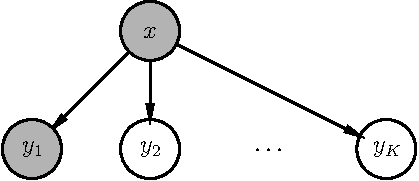
\includegraphics[width=.8\textwidth]{mmclassifier.pdf} % textwidth in subfigure environment
        \caption{Multi-class multi-label classifier}
    \end{subfigure}
    \begin{subfigure}[t]{.33\textwidth}
        \centering
        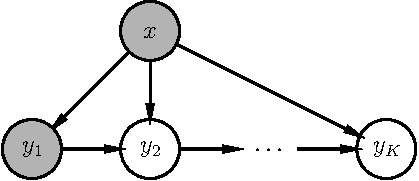
\includegraphics[width=.8\textwidth]{memm.pdf}
        \caption{MEMM}
    \end{subfigure}
    \begin{subfigure}[t]{.33\textwidth}
        \centering
        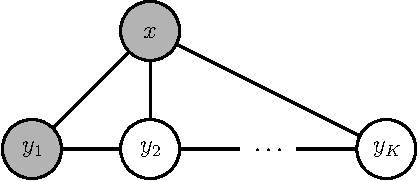
\includegraphics[width=.8\textwidth]{crf.pdf}
        \caption{CRF}
    \end{subfigure}
    \caption{Graphical models for trajectory recommendation.}
    \label{fig:pgm}
\end{figure}


\subsubsection{Maximum-entropy Markov models}
\label{sec:memm}

For MEMM, the compatibility function $f(\mathbf{x}, \mathbf{y})$ is the probability of trajectory $\mathbf{y}$ given query $\mathbf{x} = (s, K)$,
\begin{equation*}
f(\mathbf{x}, \mathbf{y}) 
= \mathbb{P}(\mathbf{y} \given \mathbf{x}; \mathbf{w}) 
= \mathbb{P}(y_1 \given \mathbf{x}; \mathbf{w}) \cdot \prod_{j=2}^K \mathbb{P}(y_j \given y_{j-1}, \mathbf{x}; \mathbf{w})
= 1 \cdot \prod_{j=2}^{K}~
  \frac{\exp \left(\mathbf{w}^\top \Psi_j(\mathbf{x}, y_{j-1}, y_j) \right)}
       {\sum_{y' \in \mathcal{P}} \exp \left(\mathbf{w}^\top \Psi_j(\mathbf{x}, y_{j-1}, y') \right)},
\end{equation*}
where we do local normalisation.

The negative log-likelihood of training set is
\begin{equation*}
\ell(\mathbf{w}) 
= -\sum_{i=1}^N \log \mathbb{P}(\mathbf{y}^{(i)} \given \mathbf{x}^{(i)}; \mathbf{w}) \\
= -\sum_{i=1}^N \sum_{j=2}^{| \mathbf{y}^{(i)} |} 
                \mathbf{w}^\top \Psi_j(\mathbf{x}^{(i)}, y_{j-1}^{(i)}, y_j^{(i)}) +
   \sum_{i=1}^N \sum_{j=2}^{| \mathbf{y}^{(i)} |} 
                \log \sum_{y' \in \mathcal{P}} \exp \left(\mathbf{w}^\top \Psi_j(\mathbf{x}^{(i)}, y_{j-1}^{(i)}, y') \right).
\end{equation*}

To learn the parameters, we maximise the likelihood of training set by minimising its negative log-likelihood (with L2 regularisation)
\begin{equation}
\label{eq:trainmemm}
\min_{\mathbf{w}} \frac{1}{2} \mathbf{w}^\top \mathbf{w} + C \ell(\mathbf{w}).
\end{equation}

A straightforward approach to optimise the above objective is employing gradient descent. 
Let $J(\mathbf{w})$ be the objective (cost function), i.e.,
\begin{align*}
J(\mathbf{w}) 
&= \frac{1}{2} \mathbf{w}^\top \mathbf{w} + C \ell(\mathbf{w}) \\
&= \frac{1}{2} \mathbf{w}^\top \mathbf{w} -
   C \sum_{i=1}^N \sum_{j=2}^{| \mathbf{y}^{(i)} |} \mathbf{w}^\top \Psi_j(\mathbf{x}^{(i)}, y_{j-1}^{(i)}, y_j^{(i)}) +
   C \sum_{i=1}^N \sum_{j=2}^{| \mathbf{y}^{(i)} |} \log \sum_{y' \in \mathcal{P}} 
     \exp \left(\mathbf{w}^\top \Psi_j(\mathbf{x}^{(i)}, y_{j-1}^{(i)}, y') \right).
\end{align*}
The gradient of the cost function w.r.t. parameters $\mathbf{w}$ is
\begin{align*}
\frac{\partial J{\mathbf{w}}}{\partial \mathbf{w}}
&= \mathbf{w} + C \frac{\partial \ell(\mathbf{w})}{\partial \mathbf{w}} \\
&= \mathbf{w} - C \sum_{i=1}^N \sum_{j=2}^{| \mathbf{y}^{(i)} |} \Psi_j(\mathbf{x}^{(i)}, y_{j-1}^{(i)}, y_j^{(i)}) +
   C \sum_{i=1}^N \sum_{j=2}^{| \mathbf{y}^{(i)} |} 
     \frac{\sum_{y' \in \mathcal{P}} \left( \Psi_j(\mathbf{x}^{(i)}, y_{j-1}^{(i)}, y') \cdot 
           \exp \left(\mathbf{w}^\top \Psi_j(\mathbf{x}^{(i)}, y_{j-1}^{(i)}, y') \right) \right)}
          {\sum_{y' \in \mathcal{P}} \exp \left(\mathbf{w}^\top \Psi_j(\mathbf{x}^{(i)}, y_{j-1}^{(i)}, y') \right)}.
\end{align*}


MEMM is a directed graphical model (as shown in Figure~\ref{fig:pgm}(b)) which captures transitions from one POI to any other POIs simultaneously, 
in contrast, pairwise ranking (Section~\ref{sec:rank}) captures only pairwise relations independently.

To make a prediction, we need to do a MAP inference (which can be done using the Viterbi algorithm if duplicated POIs are permitted)
\begin{equation}
\label{eq:testmemm}
\begin{aligned}
\mathbf{y}^* 
&= \argmax_{\mathbf{y} \in \mathcal{Y}_\mathbf{x}}~f(\mathbf{x}, \mathbf{y})
 = \argmax_{\mathbf{y} \in \mathcal{Y}_\mathbf{x}}~\mathbb{P}(\mathbf{y} \given \mathbf{x}; \mathbf{w})
 = \argmax_{\mathbf{y} \in \mathcal{Y}_\mathbf{x}}~\log \mathbb{P}(\mathbf{y} \given \mathbf{x}; \mathbf{w}) \\
&= \argmax_{\mathbf{y} \in \mathcal{Y}_\mathbf{x}}~\sum_{j=2}^{K} \mathbf{w}^\top \Psi_j(\mathbf{x}, y_{j-1}, y_j) - 
   \sum_{j=2}^{K} \log \sum_{y' \in \mathcal{P}} \exp \left(\mathbf{w}^\top \Psi_j(\mathbf{x}, y_{j-1}, y') \right).
\end{aligned}
\end{equation}

Furthermore, we can explicitly model dependencies between POIs in trajectory by adding dependences between variable $y_j$ and $y_k,~ j < k$,
which results in another compatibility function
\begin{equation*}
f(\mathbf{x}, \mathbf{y}) 
= \mathbb{P}(\mathbf{y} \given \mathbf{x}; \mathbf{w}) 
= \mathbb{P}(y_1 \given \mathbf{x}; \mathbf{w}) \cdot \prod_{j=2}^K \mathbb{P}(y_j \given y_1,\dots, y_{j-1}, \mathbf{x}; \mathbf{w})
= 1 \cdot \prod_{j=2}^{K}~
  \frac{\exp \left(\mathbf{w}_j^\top \Psi_j(\mathbf{x}, y_1, \dots, y_{j-1}, y_j) \right)}
       {\sum_{y' \in \mathcal{P}} \exp \left(\mathbf{w}_j^\top \Psi_j(\mathbf{x}, y_1, \dots, y_{j-1}, y') \right)}.
\end{equation*}

It can be trained similarly using the maximum likelihood principle.



\subsubsection{Conditional random fields}
\label{sec:crf}

For linear chain CRF, the compatibility function $f(\mathbf{x}, \mathbf{y})$ is also the probability of trajectory $\mathbf{y}$ given
query $\mathbf{x} = (s, K)$,
\begin{equation*}
f(\mathbf{x}, \mathbf{y}) = \mathbb{P}(\mathbf{y} \given \mathbf{x}; \mathbf{w}) 
= \frac{\exp \left( \mathbf{w}^\top \Psi(\mathbf{x}, \mathbf{y}) \right)}
       {\sum_{\mathbf{y}' \in \mathcal{Y}_\mathbf{x}} \exp \left( \mathbf{w}^\top \Psi(\mathbf{x}, \mathbf{y}') \right)}
= \frac{\prod_{j=2}^{K} \exp \left( \mathbf{w}_j^\top \Psi_j(\mathbf{x}, y_{j-1}, y_j) \right)}
       {\sum_{\mathbf{y}' \in \mathcal{Y}_\mathbf{x}} \prod_{j=2}^{K} \exp \left( \mathbf{w}_j^\top \Psi_j(\mathbf{x}, y_{j-1}', y_j') \right)},
\end{equation*}
where $\mathbf{y} \in \mathcal{Y}_\mathbf{x}$ and we assume decomposition 
$\mathbf{w}^\top \Psi(\mathbf{x}, \mathbf{y}) = \sum_{j=2}^{K} \mathbf{w}_j^\top \Psi_j(\mathbf{x}, y_{j-1}, y_j)$.
The denominator is known as the \emph{partition function} and we do global normalisation.

The negative log-likelihood of training set is
\begin{equation*}
\ell(\mathbf{w}) 
= -\sum_{i=1}^N \log \mathbb{P}(\mathbf{y}^{(i)} \given \mathbf{x}^{(i)}; \mathbf{w})
= -\sum_{i=1}^N \sum_{j=2}^{| \mathbf{y}^{(i)} |} \mathbf{w}_j^\top \Psi_j(\mathbf{x}^{(i)}, y_{j-1}^{(i)}, y_j^{(i)}) +
   \sum_{i=1}^N \log \sum_{\mathbf{y}' \in \mathcal{Y}_\mathbf{x}} 
                \prod_{j=2}^{K} \exp \left(\mathbf{w}_j^\top \Psi_j(\mathbf{x}^{(i)}, y_{j-1}', y_j')\right).
\end{equation*}

To learn the parameters, we maximise the likelihood of training set by minimising its negative log-likelihood (with L2 regularisation)
\begin{equation}
\label{eq:traincrf}
\min_{\mathbf{w}} \frac{1}{2} \mathbf{w}^\top \mathbf{w} + C \ell(\mathbf{w}).
\end{equation}

CRF is an undirected graphical model as shown in Figure~\ref{fig:pgm}(c).
Similar to MEMM, CRF can capture transitions from one POI to any other POIs simultaneously.
To make a prediction, we need to do a MAP inference
\begin{equation}
\label{eq:testcrf}
\begin{aligned}
\mathbf{y}^* 
&= \argmax_{\mathbf{y} \in \mathcal{Y}_\mathbf{x}}~f(\mathbf{x}, \mathbf{y})
 = \argmax_{\mathbf{y} \in \mathcal{Y}_\mathbf{x}}~\mathbb{P}(\mathbf{y} \given \mathbf{x}; \mathbf{w})
 = \argmax_{\mathbf{y} \in \mathcal{Y}_\mathbf{x}}~\log \mathbb{P}(\mathbf{y} \given \mathbf{x}; \mathbf{w}) \\
&= \argmax_{\mathbf{y} \in \mathcal{Y}_\mathbf{x}}~\sum_{j=2}^{K} \mathbf{w}_j^\top \Psi_j(\mathbf{x}, y_{j-1}, y_j) -
   \log \sum_{\mathbf{y}' \in \mathcal{Y}_\mathbf{x}} \prod_{j=2}^{K} \exp \left( \mathbf{w}_j^\top \Psi_j(\mathbf{x}, y_{j-1}', y_j') \right).
\end{aligned}
\end{equation}

\eat{TODO: why people usually employ CRF?}


\subsubsection{Structured SVM}
\label{sec:ssvm}

For structured SVM, the compatibility function $f(\mathbf{x}, \mathbf{y})$ is this linear form,
\begin{equation*}
f(\mathbf{x}, \mathbf{y}) = \mathbf{w}^\top \Psi(\mathbf{x}, \mathbf{y}),
\end{equation*}
where $\Psi(\mathbf{x}, \mathbf{y})$ is a \emph{joint feature map} 
that captures features extracted from both query $\mathbf{x}$ and trajectory $\mathbf{y}$.

The design of joint feature $\Psi(\cdot,\cdot)$ is problem specific, 
for trajectory recommendation, we assume decomposition
\begin{equation*}
\label{eq:jointfeature}
\mathbf{w}^\top \Psi(\mathbf{x}, \mathbf{y}) 
= \sum_{j=2}^{| \mathbf{y} |} 
  \left( \mathbf{w}_j^\top \Psi_j(\mathbf{x}, y_j) + 
  \mathbf{w}_{j-1,j}^\top \Psi_{j-1, j}(\mathbf{x}, y_{j-1}, y_j) \right),
\end{equation*}
where $\Psi_j$ is a feature vector of POI $y_j$ (w.r.t. query $\mathbf{x}$)
and $\Psi_{j-1,j}$ is a pairwise feature vector that captures the affinity of transition from POI $y_{j-1}$ to POI $y_j$.

To learn the parameters, we train the structured SVM by optimising a quadratic program (QP),
\begin{equation}
\label{eq:nslack}
\begin{aligned}
\min_{\mathbf{w}, ~\bm{\xi} \ge 0} ~& \frac{1}{2} \mathbf{w}^\top \mathbf{w} + \frac{C}{N} \sum_{i=1}^N \xi_i \\
s.t.~~ ~& \mathbf{w}^\top \Psi(\mathbf{x}^{(i)}, \mathbf{y}^{(i)}) - \mathbf{w}^\top \Psi(\mathbf{x}^{(i)}, \bar{\mathbf{y}}) \ge 
       \Delta(\mathbf{y}^{(i)}, \bar{\mathbf{y}}) - \xi_i, ~\bar{\mathbf{y}} \in \mathcal{Y}_{\mathbf{x}^{(i)}},~\forall i,
\end{aligned}
\end{equation}
where $\Delta(\mathbf{y}, \bar{\mathbf{y}})$ is a discrepancy function that measures the loss 
for predicting $\bar{\mathbf{y}}$ given ground truth $\mathbf{y}$, 
and slack variable $\xi_i$ is the \emph{hinge loss} for the prediction of the $i$-th example~\cite{tsochantaridis2005large},
\begin{equation*}
\xi_i = \max \left( 0,~ 
        \max_{\bar{\mathbf{y}} \in \mathcal{Y}_{\mathbf{x}^{(i)}}} 
        \left\{ \Delta(\mathbf{y}^{(i)}, \bar{\mathbf{y}}) + \mathbf{w}^\top \Psi(\mathbf{x}^{(i)}, \bar{\mathbf{y}}) \right\} -
        \mathbf{w}^\top \Psi(\mathbf{x}^{(i)}, \mathbf{y}^{(i)}) \right).
\end{equation*}
%This formulation is called "$n$-slack" as we have one slack variable for each example in training set.

We can rewrite the constraint in problem (\ref{eq:nslack}) as
\begin{equation}
\label{eq:ssvminf}
\mathbf{w}^\top \Psi(\mathbf{x}^{(i)}, \mathbf{y}^{(i)}) + \xi_i \ge
          \max_{\bar{\mathbf{y}} \in \mathcal{Y}_{\mathbf{x}^{(i)}}}
          \left\{\mathbf{w}^\top \Psi(\mathbf{x}^{(i)}, \bar{\mathbf{y}}) + \Delta(\mathbf{y}^{(i)}, \bar{\mathbf{y}}) \right\},~ \forall i,
\end{equation}
where the right hand side is known as the \emph{loss-augmented inference}.

To solve problem (\ref{eq:nslack}), one option is simply enumerating all constraints, and feeding the problem into a standard QP solver.
However, this approach is impractical as there is a constraint for every possible label $\bar{\mathbf{y}}$.
Instead, we use a cutting-plane algorithm which repeatedly solves QP (\ref{eq:nslack}) 
w.r.t. different set of constraints~\cite{joachims2009predicting}.
In each iteration, a new constraint is formed by solving the loss-augmented inference, 
which helps shrink the feasible region of the problem.

\paragraph{Multi-label SSVM}
Given a query $\mathbf{x} = (s, K)$, we normally observed more than one trajectories, which is different from the one-to-one correspondence 
between feature vectors and labels in the classification setting.
We can model this multi-label setting with a multi-label SSVM, in other words,
for each query $\mathbf{x}^{(i)}$, we have multiple labels $\mathbf{y}^{(ij)}, j=1,\dots,n_i$ 
where $n_i$ is the number of labels for query $\mathbf{x}_i$ in training set. 

We can train this multi-label SSVM by optimising a QP similar to (\ref{eq:nslack}),
\begin{equation}
\label{eq:nslack_ml}
\begin{aligned}
\min_{\mathbf{w}, ~\bm{\xi} \ge 0} ~& \frac{1}{2} \mathbf{w}^\top \mathbf{w} + \frac{C}{N} \sum_{i=1}^N \xi_{ij} \\
s.t.~~ ~& \mathbf{w}^\top \Psi(\mathbf{x}^{(i)}, \mathbf{y}^{(ij)}) - \mathbf{w}^\top \Psi(\mathbf{x}^{(i)}, \bar{\mathbf{y}}) \ge 
       \Delta(\mathbf{y}^{(ij)}, \bar{\mathbf{y}}) - \xi_{ij}, 
~\bar{\mathbf{y}} \in \mathcal{Y}_{\mathbf{x}^{(i)}} \setminus \{\mathbf{y}^{(ij)}\}_{j=1}^{n_i},~\forall j,~\forall i.
\end{aligned}
\end{equation}


\paragraph{Multi-user multi-label SSVM}
We can extend the multi-label SSVM (\ref{eq:nslack_ml}) to the multi-user setting.
In particular, let $I$ denotes the number of users,  $J_i$ denotes the number of queries of the  $i$-th user and 
$K_{ij}$ denotes the number of labels/trajectories of the $j$-th query of the $i$-th user.
Suppose the parameters/weights for the $i$-th user is $(\mathbf{\bar{w}} + \mathbf{w}_i)$ where 
$\mathbf{\bar{w}}$ is a weight vector shared by all users,
the 1-slack formulation of multi-user multi-label SSVM is the following QP:
\begin{equation}
\label{eq:1slack_muml}
\begin{aligned}
\min_{\mathbf{\bar{w}}, \mathbf{w}_i, \xi \ge 0} ~& \frac{1}{2} \mathbf{\bar{w}}^\top \mathbf{\bar{w}} + 
                                                    \frac{1}{2} \sum_{i=1}^I \mathbf{w}_i^\top \mathbf{w}_i + C \xi \\
s.t.~~~~ ~& \frac{1}{N} \sum_{i=1}^I \sum_{j=1}^{J_i} \sum_{k=1}^{K_{ij}} 
            \langle \mathbf{\bar{w}} + \mathbf{w}_i,~ \Psi(\mathbf{x}_{ij}, \mathbf{y}_{ijk}) - \Psi(\mathbf{x}_{ij}, \mathbf{\bar{y}}) \rangle \ge
            \frac{1}{N} \sum_{i=1}^I \sum_{j=1}^{J_i} \sum_{k=1}^{K_{ij}} \Delta(\mathbf{y}_{ijk}, \mathbf{\bar{y}}) - \xi,~~ 
            \mathbf{\bar{y}} \in \mathcal{Y}_{\mathbf{x}_{ij}} \setminus \{\mathbf{y}_{ijk}\}_{\forall k}
\end{aligned}
\end{equation}
where $N = \sum_{i=1}^I \sum_{j=1}^{J_i} K_{ij}$ is the total number of all observed trajectories.

To solve problem (\ref{eq:1slack_muml}) using cutting plane algorithm and a QP solver, we need the Wolfe-dual of (\ref{eq:1slack_muml}).
The Lagrangian of (\ref{eq:1slack_muml}) is 
\begin{equation}
\label{eq:lagrangian}
L(\mathbf{\bar{w}}, \mathbf{w}_i, \bm{\alpha}) 
= \frac{1}{2} \mathbf{\bar{w}}^\top \mathbf{\bar{w}} + \frac{1}{2} \sum_{i=1}^I \mathbf{w}_i^\top \mathbf{w}_i + C \xi + 
  \sum_{\mathbf{\bar{y}}} \alpha_{\mathbf{\bar{y}}} \left( 
  \frac{1}{N} \sum_{i=1}^I \sum_{j=1}^{J_i} \sum_{k=1}^{K_{ij}} \Delta(\mathbf{y}_{ijk}, \mathbf{\bar{y}}) - \xi - 
  \frac{1}{N} \sum_{i=1}^I \sum_{j=1}^{J_i} \sum_{k=1}^{K_{ij}}
  \langle \mathbf{\bar{w}} + \mathbf{w}_i,~ \Psi(\mathbf{x}_{ij}, \mathbf{y}_{ijk}) - \Psi(\mathbf{x}_{ij}, \mathbf{\bar{y}}) \rangle \right)
\end{equation}
Differentiating with respect to $\mathbf{\bar{w}}, \mathbf{w}_i$ and $\xi$, 
\begin{align*}
\frac{\partial L}{\partial \mathbf{\bar{w}}} 
&= \mathbf{\bar{w}} + \sum_{\mathbf{\bar{y}}} \alpha_{\mathbf{\bar{y}}} 
   \left( -\frac{1}{N} \sum_{i=1}^I \sum_{j=1}^{J_i} \sum_{k=1}^{K_{ij}}
   \left( \Psi(\mathbf{x}_{ij}, \mathbf{y}_{ijk}) - \Psi(\mathbf{x}_{ij}, \mathbf{\bar{y}}) \right) \right), \\
\frac{\partial L}{\partial \mathbf{w}_i} 
&= \mathbf{w}_i + \sum_{\mathbf{\bar{y}}} \alpha_{\mathbf{\bar{y}}} 
   \left( -\frac{1}{N} \sum_{j=1}^{J_i} \sum_{k=1}^{K_{ij}}
   \left( \Psi(\mathbf{x}_{ij}, \mathbf{y}_{ijk}) - \Psi(\mathbf{x}_{ij}, \mathbf{\bar{y}}) \right) \right), \\
\frac{\partial L}{\partial \xi}
&= C + \sum_{\mathbf{\bar{y}}} \alpha_{\mathbf{\bar{y}}} (-1),
\end{align*}
and setting the derivatives to zero, we have
\begin{equation}
\label{eq:equalities}
\begin{aligned}
\mathbf{\bar{w}} 
&= \sum_{\mathbf{\bar{y}}} \alpha_{\mathbf{\bar{y}}} 
   \left( \frac{1}{N} \sum_{i=1}^I \sum_{j=1}^{J_i} \sum_{k=1}^{K_{ij}}
   \left( \Psi(\mathbf{x}_{ij}, \mathbf{y}_{ijk}) - \Psi(\mathbf{x}_{ij}, \mathbf{\bar{y}}) \right) \right), \\
\mathbf{w}_i 
&= \sum_{\mathbf{\bar{y}}} \alpha_{\mathbf{\bar{y}}} 
   \left( \frac{1}{N} \sum_{j=1}^{J_i} \sum_{k=1}^{K_{ij}}
   \left( \Psi(\mathbf{x}_{ij}, \mathbf{y}_{ijk}) - \Psi(\mathbf{x}_{ij}, \mathbf{\bar{y}}) \right) \right), \\
C
&= \sum_{\mathbf{\bar{y}}} \alpha_{\mathbf{\bar{y}}}.
\end{aligned}
\end{equation}
Plugging these equalities into the Lagrangian (\ref{eq:lagrangian}), we obtain the objective of the dual problem:
\begin{equation}
\label{eq:dual_obj}
\begin{aligned}
D(\bm{\alpha})
=& \frac{1}{2} \mathbf{\bar{w}}^\top \mathbf{\bar{w}} + \frac{1}{2} \sum_{i=1}^I \mathbf{w}_i^\top \mathbf{w}_i + 
   \sum_{\mathbf{\bar{y}}} \alpha_{\mathbf{\bar{y}}}
   \left( \frac{1}{N} \sum_{i=1}^I \sum_{j=1}^{J_i} \sum_{k=1}^{K_{ij}} 
   \Delta(\mathbf{y}_{ijk}, \mathbf{\bar{y}}) \right) - \mathbf{\bar{w}}^\top \mathbf{\bar{w}} -
   \sum_{\mathbf{\bar{y}}} \alpha_{\mathbf{\bar{y}}} \left( \frac{1}{N} \sum_{i=1}^I \mathbf{w}_i^\top 
   \left[ \sum_{j=1}^{J_i} \sum_{k=1}^{K_{ij}} 
   \left( \Psi(\mathbf{x}_{ij}, \mathbf{y}_{ijk}) - \Psi(\mathbf{x}_{ij}, \mathbf{\bar{y}}) \right) \right] \right) \\
=& -\frac{1}{2} \mathbf{\bar{w}}^\top \mathbf{\bar{w}} + \frac{1}{2} \sum_{i=1}^I \mathbf{w}_i^\top \mathbf{w}_i + 
   \sum_{\mathbf{\bar{y}}} \alpha_{\mathbf{\bar{y}}} 
   \left( \frac{1}{N} \sum_{i=1}^I \sum_{j=1}^{J_i} \sum_{k=1}^{K_{ij}} 
   \Delta(\mathbf{y}_{ijk}, \mathbf{\bar{y}}) \right) - \sum_{i=1}^I \mathbf{w}_i^\top \left[
   \sum_{\mathbf{\bar{y}}} \alpha_{\mathbf{\bar{y}}} 
   \left( \frac{1}{N} \sum_{j=1}^{J_i} \sum_{k=1}^{K_{ij}} 
   \left( \Psi(\mathbf{x}_{ij}, \mathbf{y}_{ijk}) - \Psi(\mathbf{x}_{ij}, \mathbf{\bar{y}}) \right) \right) \right] \\
=& -\frac{1}{2} \mathbf{\bar{w}}^\top \mathbf{\bar{w}} + \frac{1}{2} \sum_{i=1}^I \mathbf{w}_i^\top \mathbf{w}_i + 
   \sum_{\mathbf{\bar{y}}} \alpha_{\mathbf{\bar{y}}} 
   \left( \frac{1}{N} \sum_{i=1}^I \sum_{j=1}^{J_i} \sum_{k=1}^{K_{ij}} 
   \Delta(\mathbf{y}_{ijk}, \mathbf{\bar{y}}) \right) - \sum_{i=1}^I \mathbf{w}_i^\top \mathbf{w}_i \\
=& -\frac{1}{2} \mathbf{\bar{w}}^\top \mathbf{\bar{w}} - \frac{1}{2} \sum_{i=1}^I \mathbf{w}_i^\top \mathbf{w}_i + 
   \sum_{\mathbf{\bar{y}}} \alpha_{\mathbf{\bar{y}}} 
   \left( \frac{1}{N} \sum_{i=1}^I \sum_{j=1}^{J_i} \sum_{k=1}^{K_{ij}} 
   \Delta(\mathbf{y}_{ijk}, \mathbf{\bar{y}}) \right) \\
=& -\frac{1}{2} \left[
   \sum_{\mathbf{\bar{y}}} \alpha_{\mathbf{\bar{y}}} 
   \left( \frac{1}{N} \sum_{i=1}^I \sum_{j=1}^{J_i} \sum_{k=1}^{K_{ij}} 
   \left( \Psi(\mathbf{x}_{ij}, \mathbf{y}_{ijk}) - \Psi(\mathbf{x}_{ij}, \mathbf{\bar{y}}) \right) \right) \right]^\top \left[
   \sum_{\mathbf{\bar{y}}} \alpha_{\mathbf{\bar{y}}} 
   \left( \frac{1}{N} \sum_{i=1}^I \sum_{j=1}^{J_i} \sum_{k=1}^{K_{ij}} 
   \left( \Psi(\mathbf{x}_{ij}, \mathbf{y}_{ijk}) - \Psi(\mathbf{x}_{ij}, \mathbf{\bar{y}}) \right) \right) \right] \\
& -\frac{1}{2} \sum_{i=1}^I \left[ 
   \sum_{\mathbf{\bar{y}}} \alpha_{\mathbf{\bar{y}}}
   \left( \frac{1}{N} \sum_{j=1}^{J_i} \sum_{k=1}^{K_{ij}} 
   \left( \Psi(\mathbf{x}_{ij}, \mathbf{y}_{ijk}) - \Psi(\mathbf{x}_{ij}, \mathbf{\bar{y}}) \right) \right) \right]^\top \left[
   \sum_{\mathbf{\bar{y}}} \alpha_{\mathbf{\bar{y}}} 
   \left( \frac{1}{N} \sum_{j=1}^{J_i} \sum_{k=1}^{K_{ij}} 
   \left( \Psi(\mathbf{x}_{ij}, \mathbf{y}_{ijk}) - \Psi(\mathbf{x}_{ij}, \mathbf{\bar{y}}) \right) \right) \right] \\
& +\sum_{\mathbf{\bar{y}}} \alpha_{\mathbf{\bar{y}}} 
   \left( \frac{1}{N} \sum_{i=1}^I \sum_{j=1}^{J_i} \sum_{k=1}^{K_{ij}} 
   \Delta(\mathbf{y}_{ijk}, \mathbf{\bar{y}}) \right) \\
=& -\frac{1}{2} 
   \sum_{\mathbf{\bar{y}}} \alpha_{\mathbf{\bar{y}}} 
   \sum_{\mathbf{\bar{y}}'} \alpha_{\mathbf{\bar{y}}'} \frac{1}{N^2}
   \left[ \sum_{i=1}^I \sum_{j=1}^{J_i} \sum_{k=1}^{K_{ij}} 
   \left( \Psi(\mathbf{x}_{ij}, \mathbf{y}_{ijk}) - \Psi(\mathbf{x}_{ij}, \mathbf{\bar{y}}) \right) \right]^\top 
   \left[ \sum_{i=1}^I \sum_{j=1}^{J_i} \sum_{k=1}^{K_{ij}} 
   \left( \Psi(\mathbf{x}_{ij}, \mathbf{y}_{ijk}) - \Psi(\mathbf{x}_{ij}, \mathbf{\bar{y}}') \right) \right] \\
& -\frac{1}{2} \sum_{i=1}^I
   \sum_{\mathbf{\bar{y}}} \alpha_{\mathbf{\bar{y}}}
   \sum_{\mathbf{\bar{y}}'} \alpha_{\mathbf{\bar{y}}'} \frac{1}{N^2}
   \left[ \sum_{j=1}^{J_i} \sum_{k=1}^{K_{ij}} 
   \left( \Psi(\mathbf{x}_{ij}, \mathbf{y}_{ijk}) - \Psi(\mathbf{x}_{ij}, \mathbf{\bar{y}}) \right) \right]^\top 
   \left[ \sum_{j=1}^{J_i} \sum_{k=1}^{K_{ij}} 
   \left( \Psi(\mathbf{x}_{ij}, \mathbf{y}_{ijk}) - \Psi(\mathbf{x}_{ij}, \mathbf{\bar{y}'}) \right) \right] \\
& + \sum_{\mathbf{\bar{y}}} \alpha_{\mathbf{\bar{y}}} \left( \frac{1}{N} \sum_i \sum_j \sum_k \Delta(\mathbf{y}_{ijk}, \mathbf{\bar{y}}) \right) \\
\end{aligned}
\end{equation}

Putting (\ref{eq:equalities}) and (\ref{eq:dual_obj}) together, the dual problem is:
\begin{equation}
\label{eq:dual}
\begin{aligned}
\max_{\bm{\alpha} \ge 0} ~& D(\bm{\alpha}) \\
s.t.~~ ~& \sum_{\mathbf{\bar{y}}} \alpha_{\mathbf{\bar{y}}} = C.
\end{aligned}
\end{equation}
Note that this dual problem (\ref{eq:dual}) is also a QP and can be rewritten into the standard form
\begin{equation}
\label{eq:qp}
\begin{aligned}
\min_{x}~& \frac{1}{2}x^\top P x + q^\top x \\
s.t. ~& G x \le h \\
      & A x = b
\end{aligned}
\end{equation}

\subsubsection{Discussion}

All structured models described above suffer from a number of drawbacks.
\begin{enumerate}
\item The MEMM model (Section~\ref{sec:memm}) is relatively easy to train, 
      but the inference (Equation~\ref{eq:testmemm}) will not retain its efficiency if the no duplicates constraints are required.
\item The CRF model (Section~\ref{sec:crf}) suffers from inefficient training (Equation~\ref{eq:traincrf}) and 
      inference (Equation~\ref{eq:testcrf}) as the partition function cannot be computed efficiently.
\item Both the loss-augmented inference and prediction inference for structured SVM (Section~\ref{sec:ssvm}) cannot be done efficiently 
      if the no duplicates constraints are required.
\end{enumerate}

Approximate inference methods are critical for MEMM and CRF.
On the other hand, inference in structured SVM is equivalent to 
find a maximum-weight loop-less path with exactly $K$ edges in a complete weighted (both nodes and edges) graph, which is NP-hard (proof?).
Possible solutions including 
\begin{itemize}
\item formulating it as an integer linear program (ILP) and solve it using an ILP solver, 
      or using lazy constraint generation/cutting-plane techniques with a LP solver;
\item in addition, we can employ the list Viterbi algorithm~\cite{nilsson2001sequentially,seshadri1994list} 
      which sequentially find the next best (scored) trajectory until a maximum-weight loop-less path with exactly $K$ edges is found;
\item moreover, we can employ heuristics such as greedy search or the Christofides algorithm~\cite{christofides1976} 
      when the problem has the triangle inequality property (for trajectories, indeed).
\end{itemize}
These options are applicable to MEMM (Section~\ref{sec:memm}) as well.



\subsubsection{Inference algorithms}
\label{sec:inference}

\paragraph{Integer linear program}
If we formulate an ILP to do inference and employ the sub-tour elimination constraints from TSP, we have
\begin{alignat}{5}
& \max_{u,v} ~&& \sum_{k=1}^M \mathbf{w}_k^\top \phi_k(\mathbf{x}, p_k) \sum_{j=1}^M u_{jk} + 
                 \sum_{j=1}^M \sum_{k=1}^M u_{jk} \mathbf{w}_{jk}^\top \phi_{j, k}(\mathbf{x}, p_j, p_k) \\
& s.t. ~~ ~&& u_{jk}, ~z_j \in \{0, 1\}, ~u_{jj}=0, ~z_1=0, ~v_j \in \mathbf{Z},~ p_j \in \mathcal{P}, ~\forall j, k = 1,\cdots,M   \label{eq:cons1} \\
&          && \sum_{k=2}^M u_{1k} = 1, ~\sum_{j=2}^M u_{j1} = 0  \label{eq:cons2} \\
&          && \sum_{j=1}^M u_{jl} = z_l + \sum_{k=2}^M u_{lk} \le 1,   ~\forall l=2,\cdots,M                    \label{eq:cons3} \\
&          && \sum_{j=1}^M \sum_{k=1}^M u_{jk} = L-1,                                                           \label{eq:cons4} \\
&          && v_j - v_k + 1 \le (M-1) (1-u_{jk}),                     \forall j,k=2,\cdots,M                    \label{eq:cons5}
\end{alignat}
where $u_{jk}$ is a binary decision variable that determines whether the transition from $p_j$ to $p_k$ is in the resulting trajectory,
$z_j$ is a binary decision variable that determines whether $p_j$ is the last POI in trajectory.
$L$ is the number of POIs in trajectory.
For brevity, we arrange the POIs such that $p_1 = s$.
Firstly, the desired trajectory should start from $s$ (Constraint~\ref{eq:cons2}).
In addition, any POI could be visited at most once (Constraint~\ref{eq:cons3}).
Moreover, only $L-1$ transitions between POIs are permitted (Constraint~\ref{eq:cons4}),
i.e., the number of POI visits should be exactly $L$ (including $s$).
The last constraint, where $v_i$ is an auxiliary variable,
enforces that only a single sequence of POIs without sub-tours is permitted in the trajectory.

If we employ the above ILP to do loss-augmented inference, we can simply add a linear loss function to the objective, 
e.g., $\Delta(\mathbf{y}, \bar{\mathbf{y}}) = 1 - \sum_{j=1}^M \sum_{k=1}^M u_{j, y_k}$ if we define the loss as the number of mispredicted POIs,
where $\mathbf{y}$ is the ground truth and $\bar{\mathbf{y}}$ is the trajectory corresponding to the optimal solution of this ILP.

\paragraph{The list Viterbi algorithm}
Instead of employ an algorithm with exponential time complexity (e.g., ILP) to do inference,
we can resort to an iterative algorithm such as the list Viterbi algorithm~\cite{nilsson2001sequentially,seshadri1994list}
which sequentially find the $k$-th best (scored) trajectory given the best, $2$nd best, \dots, $(k-1)$-th best (scored) trajectories,
as described in Algorithm~\ref{alg:listviterbi}.


\begin{algorithm}[htbp]
\caption{The list Viterbi algorithm for inference}
\label{alg:listviterbi}
\begin{algorithmic}[1]
\STATE \textbf{Input}: $\mathbf{x}=(s, K),~ \mathcal{P},~ \mathbf{w},~ \Psi$
%\STATE Initialise score matrices $\alpha,~ \beta,~ f_t,~ f_{t, t+1}$, a max-heap $H,~ k=0$.
\STATE Initialise score matrices $\alpha,~ \beta,~ f_{t, t+1}$, a max-heap $H,~ k=0$.
\STATE $\triangleright$ Do the forward-backward procedure~\cite{rabiner1989tutorial}
\STATE $\forall p_j \in \mathcal{P},~ \alpha_t(p_j) = 
        \begin{cases}
        0,~ t = 1 \\
        \max_{p_i \in \mathcal{P}} \left\{ \alpha_{t-1}(p_i) + \mathbf{w}_{ij}^\top \Psi_{ij}(\mathbf{x}, p_i, p_j) + 
        \mathbf{w}_j^\top \Psi_j(\mathbf{x}, p_j) \right\},~ t=2,\dots,K
        \end{cases}$

\STATE $\forall p_i \in \mathcal{P},~ \beta_t(p_i) = 
        \begin{cases}
        0,~ t = K \\
        \max_{p_j \in \mathcal{P}} \left\{ \mathbf{w}_{ij}^\top \Psi_{ij}(\mathbf{x}, p_i, p_j) + 
        \mathbf{w}_j^\top \Psi_j(\mathbf{x}, p_j) + \beta_{t+1}(p_j) \right\},~ t = K-1,\dots,1
        \end{cases}$

%\STATE $\forall p_i \in \mathcal{P},~ f_t(p_i) = \alpha_t(p_i) + \beta_t(p_i),~ t = 1,\dots,K$
\STATE $\forall p_i, p_j \in \mathcal{P},~ f_{t,t+1}(p_i, p_j) = \alpha_t(p_i) + \mathbf{w}_{ij}^\top \Psi_{ij}(\mathbf{x}, p_i, p_j) + 
                              \mathbf{w}_j^\top \Psi_j(\mathbf{x}, p_j) + \beta_{t+1}(p_j),~ t = 1,\dots,K-1$

\STATE $\triangleright$ Identify the best (scored) trajectory $\mathbf{y}^1=(y_1^1,\dots,y_K^1)$ (possibly with sub-tours)
\STATE $y_t^1 = \begin{cases}
                s,~ t = 1 \\
%                \argmax_{p \in \mathcal{P}} \left\{ f_{1,2}(s, p) \right\},~ t = 2, \\
                \argmax_{p \in \mathcal{P}} \left\{ f_{t-1,t}(y_{t-1}^1, p) \right\},~ t = 2,\dots,K
                \end{cases}$

%\STATE $r^1 = \max_{p \in \mathcal{P}} \left\{ f_K(p) \right\}~~~ \triangleright$ $r^1$ is the score/priority of $\mathbf{y}^1$
\STATE $r^1 = \max_{p \in \mathcal{P}} \left\{ \alpha_{K}(p) \right\}~~~ \triangleright$ $r^1$ is the score/priority of $\mathbf{y}^1$
\STATE $H.\textit{push}\left(r^1,~ (\mathbf{y}^1, \textsc{nil}, \emptyset) \right)$

\WHILE{$H \ne \emptyset$ \textbf{and} $k < \,|\mathcal{P}|^{K-1} - \prod_{t=2}^K (|\mathcal{P}|-t+1)$}
    \STATE $r^k,~ (\mathbf{y}^k, I, S) = H.\textit{pop}()~~~ \triangleright$ 
           $r^k$ is the score of $\mathbf{y}^k=(y_1^k,\dots,y_K^k)$, $I$ is the partition index, and $S$ is the exclude set
    \STATE $k = k + 1$
    \RETURN $\mathbf{y}^k$ if NO sub-tours in $\mathbf{y}^k$
    \STATE $\bar{I} = \begin{cases}
                      2,~ I = \textsc{nil} \\
                      I,~ \text{otherwise}
                      \end{cases}$

    \FOR{$t = \bar{I},\dots,K$}
        \STATE $\bar{S} = \begin{cases}
                          S \cup \{ y_t^k \},~ t = \bar{I} \\
                          \{ y_t^k \},~ \text{otherwise}
                          \end{cases}$

        \STATE $\bar{y}_j = \begin{cases}
                            y_j^k,~~ j=1,\dots,t-1 \\
                            %\argmax_{p \in \mathcal{P} \setminus \textit{new\_exclude\_set}} f_{t-1,t}(y_{t-1}^k, p),~ j=t \\
                            \argmax_{p \in \mathcal{P} \setminus \bar{S}} \left\{ f_{t-1,t}(y_{t-1}^k, p) \right\},~ j=t \\
                            \argmax_{p \in \mathcal{P}} \left\{ f_{j-1, j}(\bar{y}_{j-1}, p) \right\},~ j=t+1,\dots,K
                \end{cases}$
        \STATE $\bar{r} = \begin{cases}
                          f_{t-1,t}(y_{t-1}^k, \bar{y}_t),~ I = \textsc{nil} \\
                          r^k + f_{t-1,t}(y_{t-1}^k, \bar{y}_t) - f_{t-1,t}(y_{t-1}^k, y_t^k),~ \text{otherwise}
                          \end{cases}$

        $H.\textit{push}\left(\bar{r}, (\bar{\mathbf{y}}, t, \bar{S}) \right)$
    \ENDFOR
\ENDWHILE
\end{algorithmic}
\end{algorithm}



\eat{
\subsection{Other models}
\label{sec:other}
Label ranking model,
Plackett-Luce probabilistic ranking
}


\section{Features}
\label{sec:feature}

\eat{
\underline{REVISE FEATURE DESIGN}
}

The POI and query specific features extracted from trajectories are shown in Table~\ref{tab:poifeature},
features that describe the transition preference between different POIs are shown in Table~\ref{tab:tranfeature}.



\begin{table*}[ht]
\caption{Features of POI $p$ with respect to query $(s,K)$}
\label{tab:poifeature}
\centering


\setlength{\tabcolsep}{10pt} % tweak the space between columns
\begin{tabular}{l|l} \hline
\textbf{Feature}       & \textbf{Description} \\ \hline
\texttt{category}      & one-hot encoding of the category of $p$ \\
\texttt{neighbourhood} & one-hot encoding of the POI cluster that $p$ resides in \\
\texttt{popularity}    & logarithm of POI popularity of $p$ \\
\texttt{nVisit}        & logarithm of the total number of visit by all users at $p$ \\
\texttt{nPhotoTotal}   & logarithm of the total number of photos taken at $p$ \\
\texttt{nPhotoMean}    & logarithm of the average number of photos taken at $p$ \\
\texttt{nPhotoP10}     & logarithm of the $10$-th percentile of the number of photos taken at $p$ \\
\texttt{nPhotoP50}     & logarithm of the $50$-th percentile of the number of photos taken at $p$ \\
\texttt{nPhotoP90}     & logarithm of the $90$-th percentile of the number of photos taken at $p$ \\
\texttt{durationTotal} & logarithm of the accumulated visit duration at $p$ \\
\texttt{durationMean}  & logarithm of the average visit duration at $p$ \\
\texttt{durationP10}   & logarithm of the $10$-th percentile of visit duration at $p$ \\
\texttt{durationP50}   & logarithm of the $50$-th percentile of visit duration at $p$ \\
\texttt{durationP90}   & logarithm of the $90$-th percentile of visit duration at $p$ \\
\hline
%\texttt{nOccurrence}            & the number of times $p$ occurred in a trajectory that satisfies the query \\ DON'T know given new query

\texttt{trajLen}           & trajectory length $K$, i.e., the number of POIs required \\
\texttt{sameCategory}      & $1$ if the category of $p$ is the same as that of $s$, $-1$ otherwise \\
\texttt{sameNeighbourhood} & $1$ if $p$ resides in the same POI cluster as $s$, $-1$ otherwise \\
\texttt{diffPopularity}    & real-valued difference in POI popularity of $p$ from that of $s$ \\
\texttt{diffNVisit}        & real-valued difference in the total number of visit at $p$ from that at $s$ \\
\texttt{diffNPhotoTotal}   & real-valued difference in the total number of photos taken at $p$ from that at $s$ \\
\texttt{diffNPhotoMean}    & real-valued difference in the average number of photos taken at $p$ from that at $s$ \\ 
\texttt{diffNPhotoP10}     & real-valued difference in the $10$-th percentile of the number of photos taken at $p$ from that at $s$ \\
\texttt{diffNPhotoP50}     & real-valued difference in the $50$-th percentile of the number of photos taken at $p$ from that at $s$ \\
\texttt{diffNPhotoP90}     & real-valued difference in the $90$-th percentile of the number of photos taken at $p$ from that at $s$ \\
\texttt{diffDurationTotal} & real-valued difference in the accumulated visit duration from that at $s$ \\
\texttt{diffDurationMean}  & real-valued difference in average duration at $p$ from that at $s$ \\
\texttt{diffDurationP10}   & real-valued difference in the $10$-th percentile of visit duration from that at $s$ \\
\texttt{diffDurationP50}   & real-valued difference in the $50$-th percentile of visit duration from that at $s$ \\
\texttt{diffDurationP90}   & real-valued difference in the $90$-th percentile of visit duration from that at $s$ \\
\texttt{distance}          & distance between $p$ and $s$, calculated using the Haversine formula \\
\hline
\end{tabular}
\end{table*}



\begin{table}[ht]
\caption{POI features used to estimate the (feature-wise) transition probabilities}
\label{tab:tranfeature}
\centering
%\setlength{\tabcolsep}{28pt} % tweak the space between columns
\begin{tabular}{l|l} \hline
\textbf{Feature}       & \textbf{Description} \\ \hline
\texttt{category}      & category of POI \\
\texttt{neighbourhood} & the cluster that a POI resides in \\
\texttt{popularity}    & (discretised) popularity of POI \\
\texttt{nVisit}        & (discretised) total number of visit at POI \\
\texttt{durationMean}  & (discretised) average duration at POI \\ \hline
\end{tabular}
\end{table}

% !TEX root=main.tex

We are now in a position to empirically compare the methods discussed above,
to get a firmer sense of their tradeoffs.

%
\subsection{Description of datasets}

We used the trajectory data\footnote{\url{https://bitbucket.org/d-chen/tour-cikm16}}
extracted from Flickr photos for the cities of Glasgow, Osaka and
Toronto~\cite{ijcai15,cikm16paper}.
Each dataset comprises of a
list of trajectories, being a sequence of points of interest (POI),
as visited by various Flickr users and recorded by the geotags in photos.
Table~\ref{tab:data} summarises the profile of each dataset.
We see that most queries have more than one ground truth, making the sequence recommendation setting relevant. Further, each query has an average of 4-9, and a maximum of 30-60 trajectories (details in supplement).

% In all datasets,
% each user has on average less than two trajectories.
% This makes user-specific recommendation impractical, and also undesirable because
% a user would want different recommendations given different starting locations, and not a static recommendation no matter where she is.

% dataset stats
% \begin{table}[t]
% 	\begin{minipage}[t]{\linewidth}
% 		\resizebox{\linewidth}{!}{
% 		\setlength{\tabcolsep}{4pt} % tweak the space between columns
% 		\small
% 		\begin{tabular}{lllll|ccc|cc} \hline %{l*{9}{c}} \hline
% 		\textbf{Dataset} & \textbf{\#Traj} & \textbf{\#POIs} & \textbf{\#Users} & \textbf{\#Queries} & \textbf{\#GT=1} & \textbf{\#GT$\in [2,5]$} & \textbf{\#GT$>$5} & \textbf{\#shortTraj} & \textbf{\#longTraj} \\ \hline
% 		Glasgow          & 351              & 25              & 219              & 64                 & 23              & 22                      & 19                & 336                     & 15 \\
% 		Osaka            & 186              & 26              & 130              & 47                 & 17              & 22                      & 8                 & 178                     & 8  \\
%         Toronto          & 977              & 27              & 454              & 99                 & 30              & 33                      & 36                & 918                     & 59 \\
% 		\hline
% 		\end{tabular}%
% 		}
% 		\captionof{table}{Statistics of trajectory datasets.
%         Including the number of trajectories (\#Traj), POIs (\#POIs), users (\#Users), queries (\#Queries);
%         the number of queries with a single (\#GT=1), 2-5 (\#GT$\in$[2,5]), or more than 5 (\#GT$>$5) ground truths;
%         and profile of trajectory length, \ie less than 5 (\#shortTraj) and more than 5 POIs (\#longTraj).
%         }
% 		\label{tab:data}
% 	\end{minipage}
% \end{table}

\begin{table}[t]
	\begin{minipage}[t]{\linewidth}
		\resizebox{\linewidth}{!}{
		\setlength{\tabcolsep}{4pt} % tweak the space between columns
		\small
		\begin{tabular}{llll|cc} \hline %{l*{9}{c}} \hline
		\textbf{Dataset} & \textbf{\#Traj} & \textbf{\#POIs}  & \textbf{\#Queries}  & \textbf{\#ShortTraj} & \textbf{\#LongTraj} \\ \hline
		Glasgow          & 351              & 25              & 64                 & 336                     & 15 \\
		Osaka            & 186              & 26              & 47                 & 178                     & 8  \\
        Toronto          & 977              & 27              & 99                 & 918                     & 59 \\
		\hline
		\end{tabular}%
		}
		\captionof{table}{Statistics of trajectory datasets.
        Including the number of trajectories (\#Traj), POIs (\#POIs), queries (\#Queries);
        and the number of trajectories with length less than 5 (\#ShortTraj) and more than 5 POIs (\#LongTraj).
        }
		\label{tab:data}
	\end{minipage}
\end{table}

%
\subsection{Experimental protocol}

We compare the three methods described previously ({\sc List Viterbi}, {\sc ILP}, {\sc Heuristic}),
as well as the standard inference ({\sc Viterbi}).

We evaluate each algorithm using leave-one-query-out cross validation (LOOCV).
That is, holding out all the relevant trajectories for each query $\x^{(i)}$ (\ie $\{\y^{(i,j)}\}_{j=1}^{n_i}$) in each round.
The regularisation constant $C$ is tuned using Monte Carlo cross validation~\cite{burman1989comparative} on the training set.
We use three performance measures for POIs, sequences and ordered lists.
The {\bf F$_1$ score on points}~\cite{ijcai15} computes F$_1$ on the predicted versus seen points
without considering their relative order.
The {\bf F$_1$ score on pairs}~\cite{cikm16paper} is proposed to mitigate this by computing F$_1$ on all ordered pairs in the predicted versus ground truth sequence. %%It is 1 iff both sequences agree completely.
%The well-known rank correlation {\bf Kendall's $\tau$}~\cite{agresti2010analysis}
%computes the ratio of concordant (correctly ranked) pairs minus discordant pairs, over all possible pairs after accounting for ties.%taking care of ties.


%
\subsection{Results and discussion}

We now address the motivating questions of this work.

\textbf{How often does the top-scoring sequence have loops?}
It is first of interest to determine that the top-scoring sequence for the underlying SSVM model does in fact often contain loops.
We find that on the (Osaka, Glasgow, Toronto) datasets, the top-scoring sequence for (23.9\%, 31.2\%, 48.5\%) respectively of all queries have loops.
This confirms that with longer trajectories, even a powerful structured model cannot escape the problem of predicting sequences with loops.

% Osaka percentage of predictions with loops:
% 11 / 46 = 23.9\% \\
% Glasgow percentage of predictions with loops:
% 20 / 64 = 31.2\% \\
% Toronto percentage of predictions with loops:
% 48 / 99 = 48.5\% 

\textbf{How important is it to remove loops?}
Having confirmed that loops in the top-scoring sequence are an issue,
it is now of interest to establish that removing such loops during prediction is in fact important.
This is confirmed in Tables \ref{tab:f1-master} -- \ref{tab:pf1-master},
where we see that there can be as much as a 50\% improvement in performance over the {\sc Viterbi} baseline.

\textbf{How reliably can {\sc Heuristic} get the desired length?}
A challenge in applying {\sc Heuristic} to the trajectory recommendation problem as we have defined it
is that it may result in a trajectory of the wrong length.
Figure \ref{fig:length-christo} shows that a significant fraction of queries will have a different length to the target.

\textbf{How reliably can {\sc Heuristic} predict a good trajectory?}
Assuming one can overlook the {\sc Heuristic} producing a trajectory of possibly incorrect length,
it is then of interest as to how well it performs compared to the list Viterbi and ILP methods.
Tables \ref{tab:f1-master} -- \ref{tab:pf1-master} show that the heuristic, while sometimes competitive on the F1 measures, often
grossly underperforms compared to the more principled approaches.

%Interestingly, if Kendall's $\tau$ is the measure of interest, then the heuristic may actually be preferable to these methods.

\textbf{Which of ILP or list Viterbi is faster, and when?}
The list Viterbi and ILP methods have highly similar accuracy, with the differences owing to ties.
What about their relative runtimes?
Figure \ref{fig:inftime} shows that for shorter trajectories, the list Viterbi approach is to be preferred;
however, for longer trajectories, the ILP approach is faster.

The reason for the list Viterbi to suffer at longer trajectories is simply because this creates an exponential increase in the number of available choices, which must be searched through serially.
Of interest is that ILP approach has runtime largely independent of the trajectory length.
This indicates the branch-and-bound as well as cutting plane underpinnings of these solvers are highly scalable.

As a final note, we see that the complexity of the Heuristic is several order of magnitudes less than either of the two more advanced methods at longer trajectories.
There is thus a familiar tradeoff between time and accuracy.

% !TEX root = ./main.tex

\begin{table*}[t]\captionmoveup
     \caption{Results on trajectory recommendation datasets on best of top-10.
     %The top three rows are baselines, and the bottom four are the methods proposed in this paper.
     Higher scores are better for all metrics. Bold entries: \textbf{best} performing method for each metric; italicised entries: the \textit{second best}.
     }
     \label{tab:result}
     \centering
%%     \setlength{\tabcolsep}{3pt} % tweak the space between columns
%%     \small
     \resizebox{\linewidth}{!}{
%%     \begin{tabular}{l|cc|cc|cc} \hline
%%                         & \multicolumn{2}{|c}{\textbf{Kendall's $\tau$}}
%%                         & \multicolumn{2}{|c}{\textbf{F$_1$ score on points}}
%%                         & \multicolumn{2}{|c}{\textbf{F$_1$ score on pairs}} \\ \cline{2-7}
%%                         & Osaka & Glasgow
%%                         & Osaka & Glasgow
%%                         & Osaka & Glasgow \\ \hline
%%     \textsc{Random}     & $0.685\pm0.035$ & $0.703\pm0.029$
%%                         & $0.703\pm0.032$ & $0.731\pm0.026$
%%                         & $0.451\pm0.057$ & $0.495\pm0.046$ \\
%%     \textsc{Popularity} & $0.768\pm0.038$ & $0.748\pm0.036$
%%                         & $0.786\pm0.034$ & $0.771\pm0.033$
%%                         & $0.626\pm0.055$ & $0.623\pm0.051$ \\
%%     \textsc{PoiRank}    & $0.787\pm0.037$ & $0.830\pm0.029$
%%                         & $0.804\pm0.034$ & $0.847\pm0.025$
%%                         & $0.661\pm0.056$ & $0.726\pm0.043$ \\
%%     \midrule
%%     \textsc{SP}         & $0.749\pm0.043$ & $0.790\pm0.030$
%%                         & $0.770\pm0.039$ & $0.810\pm0.027$
%%                         & $0.620\pm0.061$ & $0.658\pm0.046$ \\
%%     \textsc{SPpath}     & $\mathit{0.791\pm0.036}$ & $0.787\pm0.029$
%%                         & $\mathit{0.809\pm0.033}$ & $0.807\pm0.026$
%%                         & $\mathit{0.664\pm0.055}$ & $0.648\pm0.045$ \\
%%     \textsc{SR}         & $0.777\pm0.036$ & $\mathbf{0.868\pm0.026}$
%%                         & $0.793\pm0.033$ & $\mathbf{0.883\pm0.023}$
%%                         & $0.637\pm0.055$ & $\mathbf{0.770\pm0.039}$ \\
%%     \textsc{SRpath}     & $\mathbf{0.803\pm0.034}$ & $\mathit{0.853\pm0.026}$
%%                         & $\mathbf{0.820\pm0.031}$ & $\mathit{0.868\pm0.023}$
%%                         & $\mathbf{0.671\pm0.053}$ & $\mathit{0.746\pm0.041}$ \\ \hline
%%     \end{tabular}
\begin{tabular}{l|cc|cc|ccc} \hline
& \multicolumn{7}{c}{\bf Kendall's $\tau$} \\ \hline
 & \textsc{Random} & \textsc{Popularity} & \textsc{PoiRank} & \textsc{SP} & \textsc{SPpath} & \textsc{SR} & \textsc{SRpath} \\ \hline
Glasgow & $0.703\pm0.029$ & $0.748\pm0.036$ & $0.830\pm0.029$ & $0.790\pm0.030$ & $0.787\pm0.029$ & $\mathbf{0.868\pm0.026}$ & $\mathit{0.853\pm0.026}$ \\
Osaka & $0.685\pm0.035$ & $0.768\pm0.038$ & $0.787\pm0.037$ & $0.749\pm0.043$ & $\mathit{0.791\pm0.036}$ & $0.777\pm0.036$ & $\mathbf{0.803\pm0.034}$ \\
Toronto & $0.652\pm0.024$ & $0.719\pm0.024$ & $0.784\pm0.023$ & $0.697\pm0.027$ & $0.719\pm0.026$ & $\mathbf{0.802\pm0.022}$ & $\mathit{0.797\pm0.022}$ \\
\hline
& \multicolumn{7}{c}{\bf F$_1$ score on points} \\ \hline
Glasgow & $0.731\pm0.026$ & $0.771\pm0.033$ & $0.847\pm0.025$ & $0.810\pm0.027$ & $0.807\pm0.026$ & $\mathbf{0.883\pm0.023}$ & $\mathit{0.868\pm0.023}$ \\
Osaka & $0.703\pm0.032$ & $0.786\pm0.034$ & $0.804\pm0.034$ & $0.770\pm0.039$ & $\mathit{0.809\pm0.033}$ & $0.793\pm0.033$ & $\mathbf{0.820\pm0.031}$ \\
Toronto & $0.696\pm0.021$ & $0.746\pm0.022$ & $0.807\pm0.020$ & $0.733\pm0.023$ & $0.755\pm0.022$ & $\mathbf{0.828\pm0.019}$ & $\mathit{0.823\pm0.020}$ \\
\hline
& \multicolumn{7}{c}{\bf F$_1$ score on pairs} \\ \hline
Glasgow & $0.495\pm0.046$ & $0.623\pm0.051$ & $0.726\pm0.043$ & $0.658\pm0.046$ & $0.648\pm0.045$ & $\mathbf{0.770\pm0.039}$ & $\mathit{0.746\pm0.041}$ \\
Osaka & $0.451\pm0.057$ & $0.626\pm0.055$ & $0.661\pm0.056$ & $0.620\pm0.061$ & $\mathit{0.664\pm0.055}$ & $0.637\pm0.055$ & $\mathbf{0.671\pm0.053}$ \\
Toronto & $0.438\pm0.034$ & $0.550\pm0.035$ & $0.649\pm0.033$ & $0.530\pm0.037$ & $0.552\pm0.036$ & $\mathbf{0.660\pm0.033}$ & $\mathit{0.657\pm0.034}$ \\
\hline
\end{tabular}
     }\eqmoveup
\end{table*}


\begin{figure*}[!t]
\begin{minipage}[c]{\textwidth}
%\begin{figure*}[!t]
		\centering
		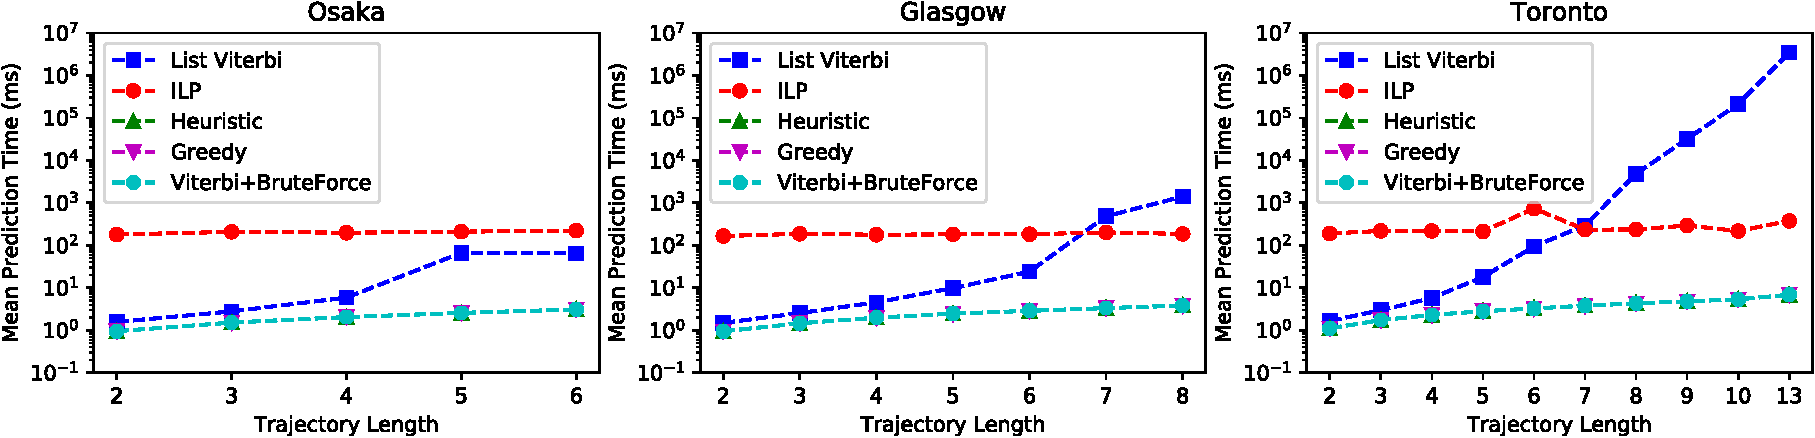
\includegraphics[width=\textwidth]{top1_inftime.pdf}
	    \captionof{figure}{Prediction time for three inference algorithms (in milliseconds)}
	    \label{fig:inftime}
	    %\captionmoveup\eqmoveup
%\end{figure*}%
%\begin{figure*}[!t]
		\quad
		\centering
		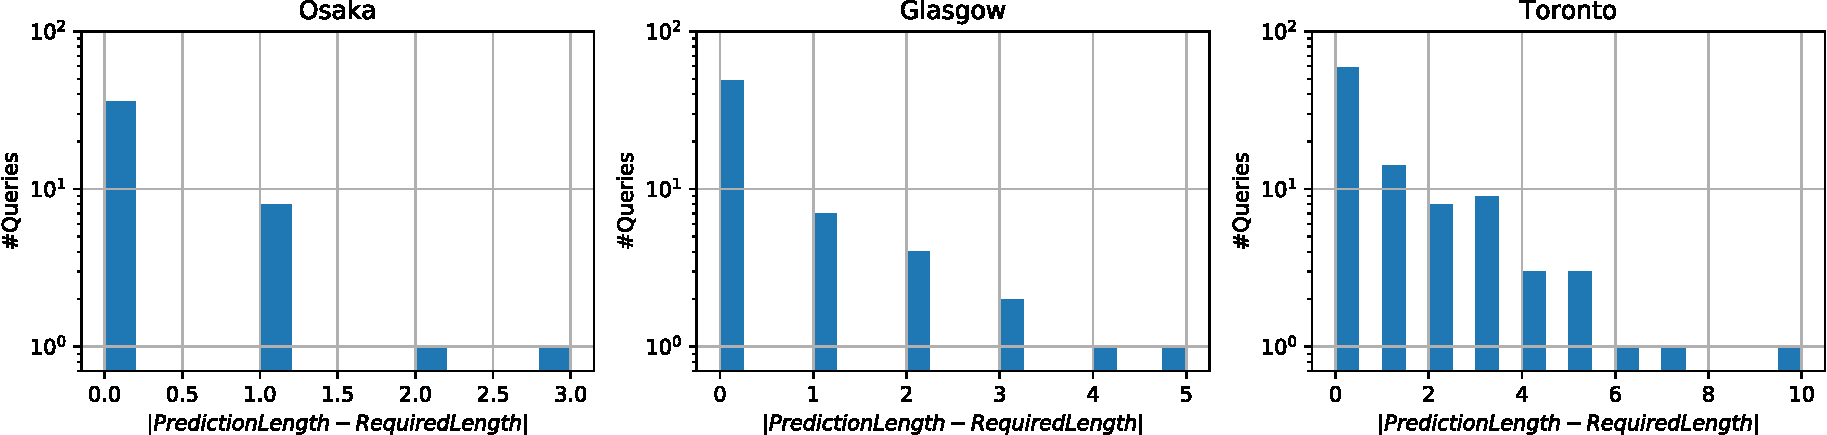
\includegraphics[width=\textwidth]{heu_lengthdiff.pdf}
	    \captionof{figure}{The difference between recommendation and required sequence length.}
	    \label{fig:length-christo}
	    %\captionmoveup\eqmoveup
%\end{figure*}%
%\begin{figure*}[!t]
		\quad
		\centering
		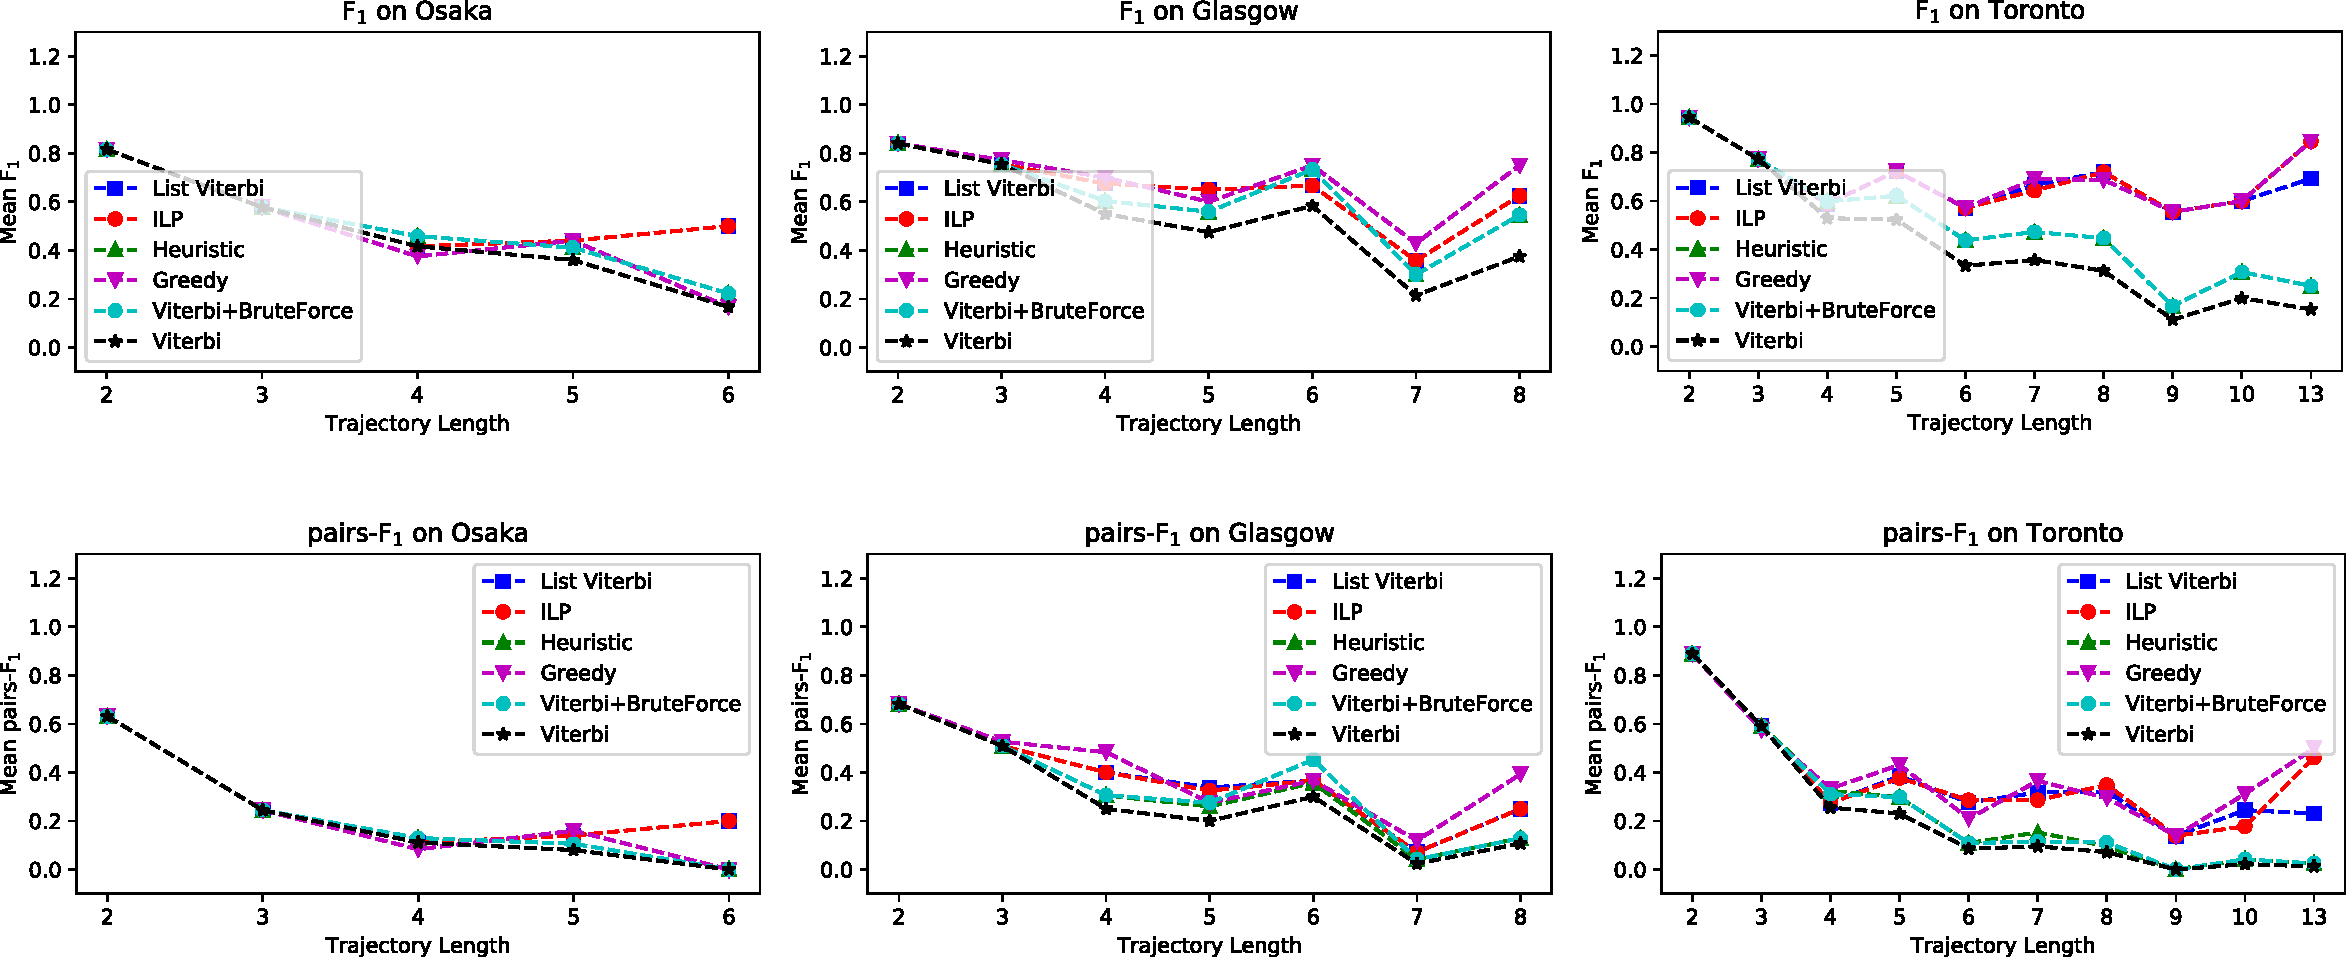
\includegraphics[width=\textwidth]{metrics.pdf}
		% 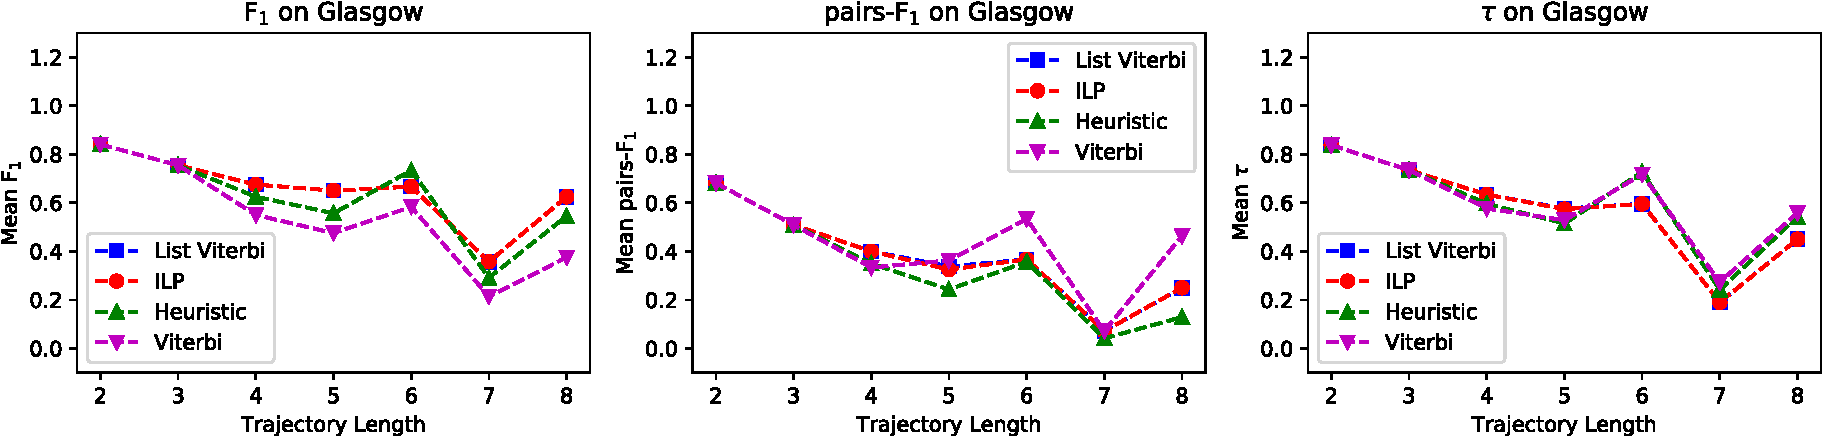
\includegraphics[width=\textwidth]{metric_d2.pdf}
		% 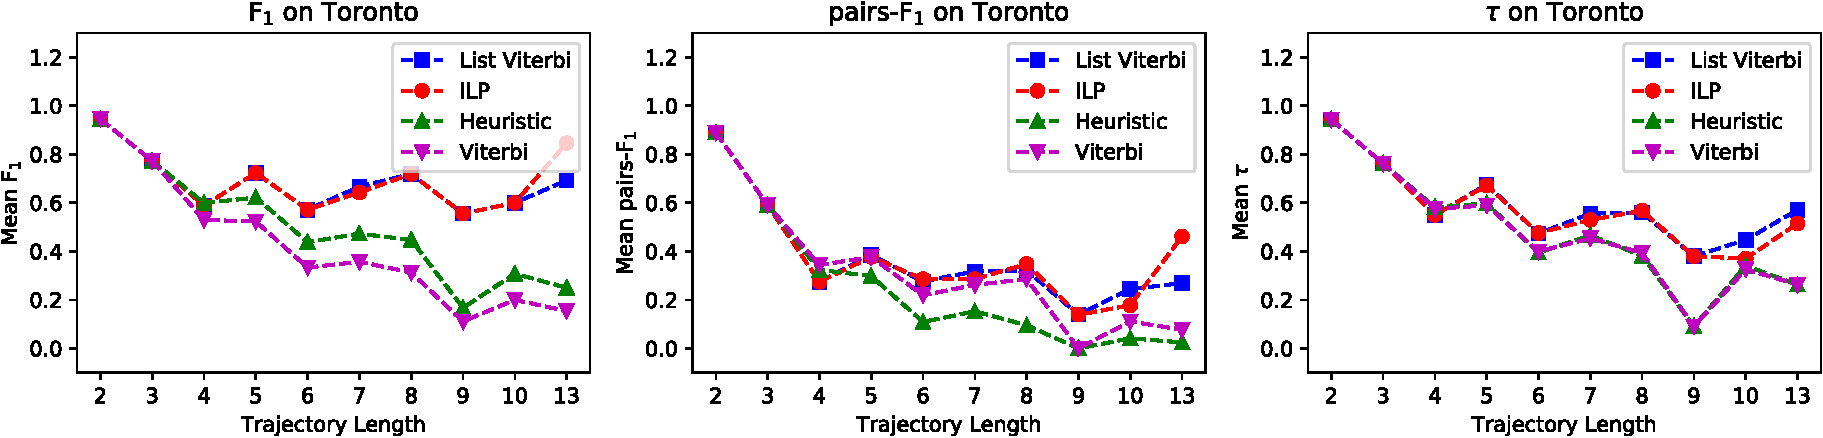
\includegraphics[width=\textwidth]{metric_d3.pdf}
	    \captionof{figure}{Accuracy versus trajectory length.}
	    \label{fig:acc-vs-length}
	    %\captionmoveup\eqmoveup
%\end{figure*}
\end{minipage}
\end{figure*}


\bibliographystyle{ieeetr}
%\bibliographystyle{apalike}
\bibliography{ref,ref_music}

\end{document}
